\documentclass [norsk,a4paper,twoside]{article}\usepackage[]{graphicx}\usepackage[]{color}
%% maxwidth is the original width if it is less than linewidth
%% otherwise use linewidth (to make sure the graphics do not exceed the margin)
\makeatletter
\def\maxwidth{ %
  \ifdim\Gin@nat@width>\linewidth
    \linewidth
  \else
    \Gin@nat@width
  \fi
}
\makeatother

\definecolor{fgcolor}{rgb}{0.345, 0.345, 0.345}
\newcommand{\hlnum}[1]{\textcolor[rgb]{0.686,0.059,0.569}{#1}}%
\newcommand{\hlstr}[1]{\textcolor[rgb]{0.192,0.494,0.8}{#1}}%
\newcommand{\hlcom}[1]{\textcolor[rgb]{0.678,0.584,0.686}{\textit{#1}}}%
\newcommand{\hlopt}[1]{\textcolor[rgb]{0,0,0}{#1}}%
\newcommand{\hlstd}[1]{\textcolor[rgb]{0.345,0.345,0.345}{#1}}%
\newcommand{\hlkwa}[1]{\textcolor[rgb]{0.161,0.373,0.58}{\textbf{#1}}}%
\newcommand{\hlkwb}[1]{\textcolor[rgb]{0.69,0.353,0.396}{#1}}%
\newcommand{\hlkwc}[1]{\textcolor[rgb]{0.333,0.667,0.333}{#1}}%
\newcommand{\hlkwd}[1]{\textcolor[rgb]{0.737,0.353,0.396}{\textbf{#1}}}%
\let\hlipl\hlkwb

\usepackage{framed}
\makeatletter
\newenvironment{kframe}{%
 \def\at@end@of@kframe{}%
 \ifinner\ifhmode%
  \def\at@end@of@kframe{\end{minipage}}%
  \begin{minipage}{\columnwidth}%
 \fi\fi%
 \def\FrameCommand##1{\hskip\@totalleftmargin \hskip-\fboxsep
 \colorbox{shadecolor}{##1}\hskip-\fboxsep
     % There is no \\@totalrightmargin, so:
     \hskip-\linewidth \hskip-\@totalleftmargin \hskip\columnwidth}%
 \MakeFramed {\advance\hsize-\width
   \@totalleftmargin\z@ \linewidth\hsize
   \@setminipage}}%
 {\par\unskip\endMakeFramed%
 \at@end@of@kframe}
\makeatother

\definecolor{shadecolor}{rgb}{.97, .97, .97}
\definecolor{messagecolor}{rgb}{0, 0, 0}
\definecolor{warningcolor}{rgb}{1, 0, 1}
\definecolor{errorcolor}{rgb}{1, 0, 0}
\newenvironment{knitrout}{}{} % an empty environment to be redefined in TeX

\usepackage{alltt}
\addtolength{\hoffset}{-0.5cm}
\addtolength{\textwidth}{1cm}
\addtolength{\voffset}{-1cm}
\addtolength{\textheight}{2cm}


%for nice looking tabs
\usepackage{booktabs}

\usepackage[norsk]{babel}
\usepackage[utf8x]{inputenc}
\usepackage{textcomp}
\usepackage{fancyhdr}
\pagestyle{fancy}
\usepackage{amsmath}
\usepackage{rotating} %add rotating for plain tables
\usepackage{pdflscape} %add rotating/landcape for pdf

%bytte font
\renewcommand{\familydefault}{\sfdefault}

%setter grå skrift fremfort sort
\usepackage{xcolor}
\usepackage{graphicx}
\usepackage[pdftex, colorlinks, linkcolor=OffBlaa3, urlcolor=OffBlaa3]{hyperref}
\IfFileExists{upquote.sty}{\usepackage{upquote}}{}
\begin{document}







\section{Oppsummeringstall for NKR}

% latex table generated in R 3.4.1 by xtable 1.8-2 package
% Wed Sep 27 11:15:26 2017
\begin{table}[ht]
\centering
\begin{tabular}{lrrrrrr}
  \hline
 & 2012 & 2013 & 2014 & 2015 & 2016 & Sum \\ 
  \hline
Ahus & 50 & 151 & 67 & 136 & 184 & 605 \\ 
  Aleris, Bergen & 217 & 265 & 145 & 95 & 59 & 939 \\ 
  Aleris, Oslo & 152 & 4 & 38 & 190 & 72 & 773 \\ 
  Arendal & 84 & 95 & 87 & 82 & 72 & 558 \\ 
  Bodø & 5 & 0 & 0 & 27 & 20 & 88 \\ 
  Bærum & 79 & 88 & 65 & 111 & 134 & 612 \\ 
  Drammen & 148 & 102 & 186 & 249 & 273 & 1108 \\ 
  Elverum & 94 & 127 & 147 & 139 & 128 & 887 \\ 
  Flekkefjord & 12 & 10 & 2 & 8 & 6 & 53 \\ 
  Førde & 0 & 0 & 0 & 0 & 25 & 32 \\ 
  Gjøvik & 85 & 74 & 94 & 75 & 118 & 643 \\ 
  Haugesund & 5 & 38 & 54 & 42 & 82 & 221 \\ 
  Haukeland, nevrokir & 158 & 170 & 186 & 168 & 170 & 1001 \\ 
  Haukeland, ort & 4 & 0 & 1 & 18 & 23 & 50 \\ 
  Ibsensykehuset & 0 & 0 & 0 & 0 & 1 & 1 \\ 
  Kolibri Medical Group & 0 & 18 & 3 & 0 & 0 & 21 \\ 
  Kristiansand & 96 & 112 & 110 & 137 & 165 & 788 \\ 
  Kristiansund & 0 & 0 & 0 & 0 & 34 & 34 \\ 
  Kysthospitalet Hagevik & 202 & 244 & 269 & 275 & 291 & 1698 \\ 
  Larvik & 29 & 0 & 0 & 0 & 117 & 202 \\ 
  Levanger & 75 & 99 & 112 & 116 & 109 & 659 \\ 
  Lillehammer & 91 & 61 & 62 & 99 & 77 & 511 \\ 
  Martina Hansens & 319 & 270 & 304 & 341 & 307 & 2006 \\ 
  Namsos & 64 & 55 & 93 & 73 & 71 & 430 \\ 
  NIMI & 27 & 24 & 129 & 111 & 116 & 458 \\ 
  Oslofjordklinikken Vest & 0 & 0 & 6 & 59 & 96 & 161 \\ 
  Oslofjordklinikken Øst & 266 & 303 & 345 & 341 & 324 & 1943 \\ 
  Rana & 10 & 19 & 23 & 23 & 30 & 145 \\ 
  Rikshospitalet, nevrokir & 37 & 52 & 55 & 63 & 33 & 400 \\ 
  Rikshospitalet, ort & 15 & 4 & 2 & 0 & 0 & 22 \\ 
  Skien & 1 & 23 & 41 & 39 & 66 & 170 \\ 
  St.Olavs, nevrokir & 345 & 325 & 346 & 356 & 299 & 2259 \\ 
  St.Olavs, ort & 58 & 46 & 50 & 32 & 39 & 350 \\ 
  Stavanger, nevrokir & 212 & 200 & 172 & 156 & 131 & 979 \\ 
  Stavanger, ort & 231 & 234 & 237 & 274 & 270 & 1331 \\ 
  Teres Colloseum, Oslo & 5 & 41 & 26 & 26 & 79 & 192 \\ 
  Teres Colloseum, Stavanger & 0 & 0 & 31 & 46 & 32 & 159 \\ 
  Teres, Bergen & 0 & 0 & 0 & 0 & 0 & 15 \\ 
  Teres, Drammen & 43 & 37 & 0 & 0 & 0 & 138 \\ 
  Ullevål, nevrokir & 34 & 80 & 30 & 42 & 88 & 274 \\ 
  Ullevål, ort & 117 & 136 & 126 & 162 & 166 & 955 \\ 
  Ulriksdal & 92 & 9 & 0 & 0 & 0 & 338 \\ 
  UNN, nevrokir & 275 & 221 & 222 & 245 & 206 & 1759 \\ 
  Volda & 24 & 29 & 27 & 38 & 31 & 170 \\ 
  Volvat & 0 & 21 & 80 & 139 & 136 & 377 \\ 
  Østfold & 0 & 0 & 61 & 48 & 44 & 153 \\ 
  Ålesund & 105 & 103 & 127 & 102 & 109 & 747 \\ 
  Sum & 3866 & 3890 & 4161 & 4683 & 4833 & 27415 \\ 
   \hline
\end{tabular}
\caption{Antall registreringer ved hver avdeling siste 5 år, samt totalt siden 2010.} 
\label{tab:AntReg}
\end{table}


Tabell \ref{tab:AntReg} viser antall 
registreringer gjort ved de respektive avdelinger hvert år. Vi ser at det er  
47 avdelinger som registrerer og at det i perioden 2010 til 2016 totalt er registrert 27415 
operasjoner. Av disse er 53.1\% utført på menn og 46.9\% på kvinner.
Siste inngrep registrert i datauttrekket som ligger til grunn for denne rapporten, ble utført 
2016-12-30. I peroden 2007 til og med 2009 er det registrert 5832 operasjoner til NKR. 

\clearpage



\section{Bakgrunnsdata}
\subsection{Alder}


% latex table generated in R 3.4.1 by xtable 1.8-2 package
% Wed Sep 27 11:15:26 2017
\begin{table}[ht]
\centering
\begin{tabular}{rlllllllll}
  \hline
 & 0-19 & 20-29 & 30-39 & 40-49 & 50-59 & 60-69 & 70-79 & 80-89 & 90+ \\ 
  \hline
Andeler & 0.4\% & 4.5\% & 11.8\% & 18.7\% & 20.3\% & 21\% & 18.9\% & 4.3\% & 0.1\% \\ 
  Antall & 21 & 216 & 569 & 898 & 976 & 1013 & 909 & 207 & 4 \\ 
   \hline
\end{tabular}
\caption{Aldersfordeling, 2016.} 
\label{tab:Alder}
\end{table}


Gjennomsnittsalderen har økt jevnt fra 53.7 år i 2010 til 56.0 år i 2016. 
Ryggkirurgi øker mest i den eldste og mest sårbare delen av
befolkningen. Disse pasientene vet vi at trenger mer omfattende utredning og
lengre liggetid. Dette medfører økte kostnader, spesielt for offentlige sykehus som i
all hovedsak håndterer denne pasientgruppen. I 2016 ble 23.3 \% (1120 operasjoner) av alle
ryggoperasjonene meldt til NKR utført på personer over 70 år.

\begin{figure}[ht]
\scalebox{0.7}{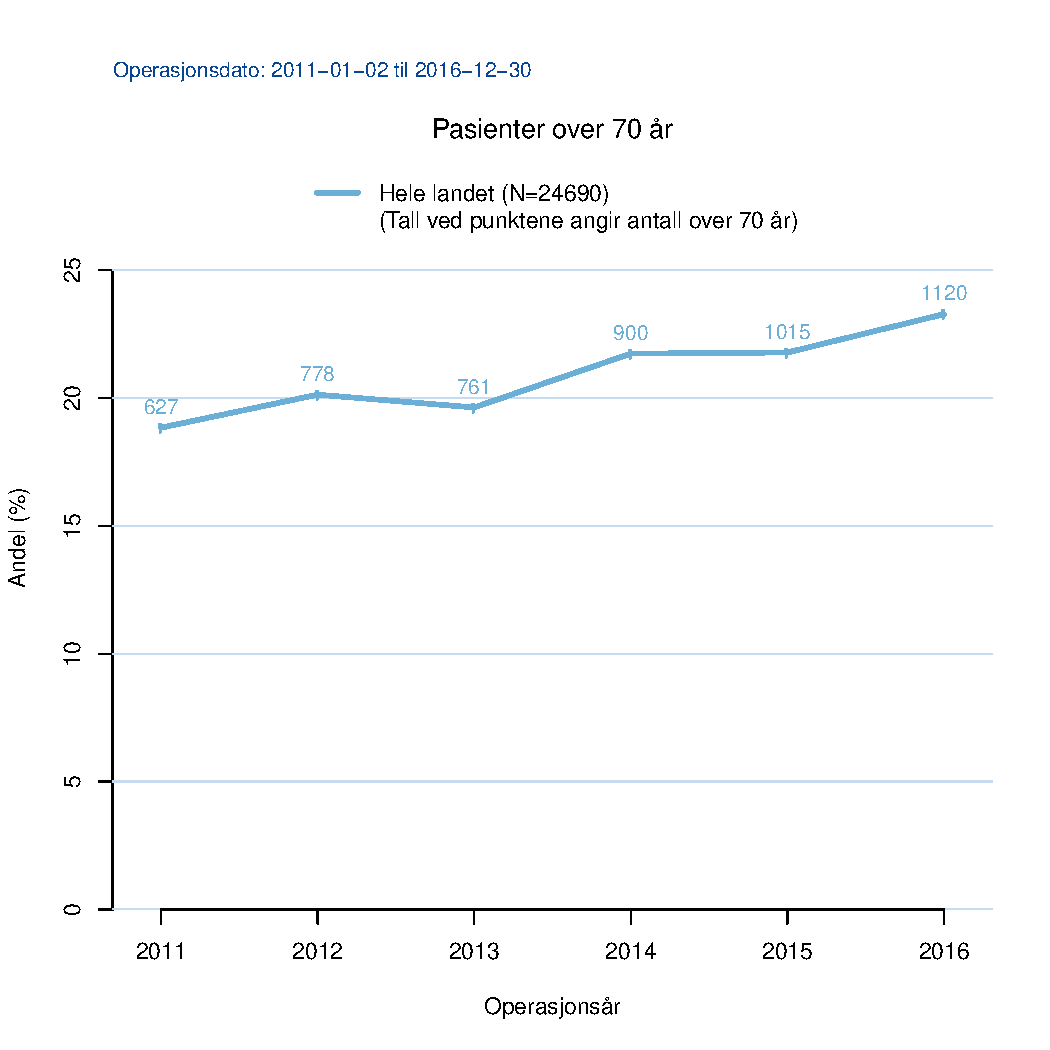
\includegraphics{Figurer/FigAlder70.pdf}}
\caption{\label{fig:Alder70} Andel ryggoperasjoner utført på personer som er 70 år eller mer.}}
\end{figure}



%Figur \ref{fig:Alder} viser aldersfordeling for alle pasienter i rappAar.

%\begin{figure}[ht]
%	\centering 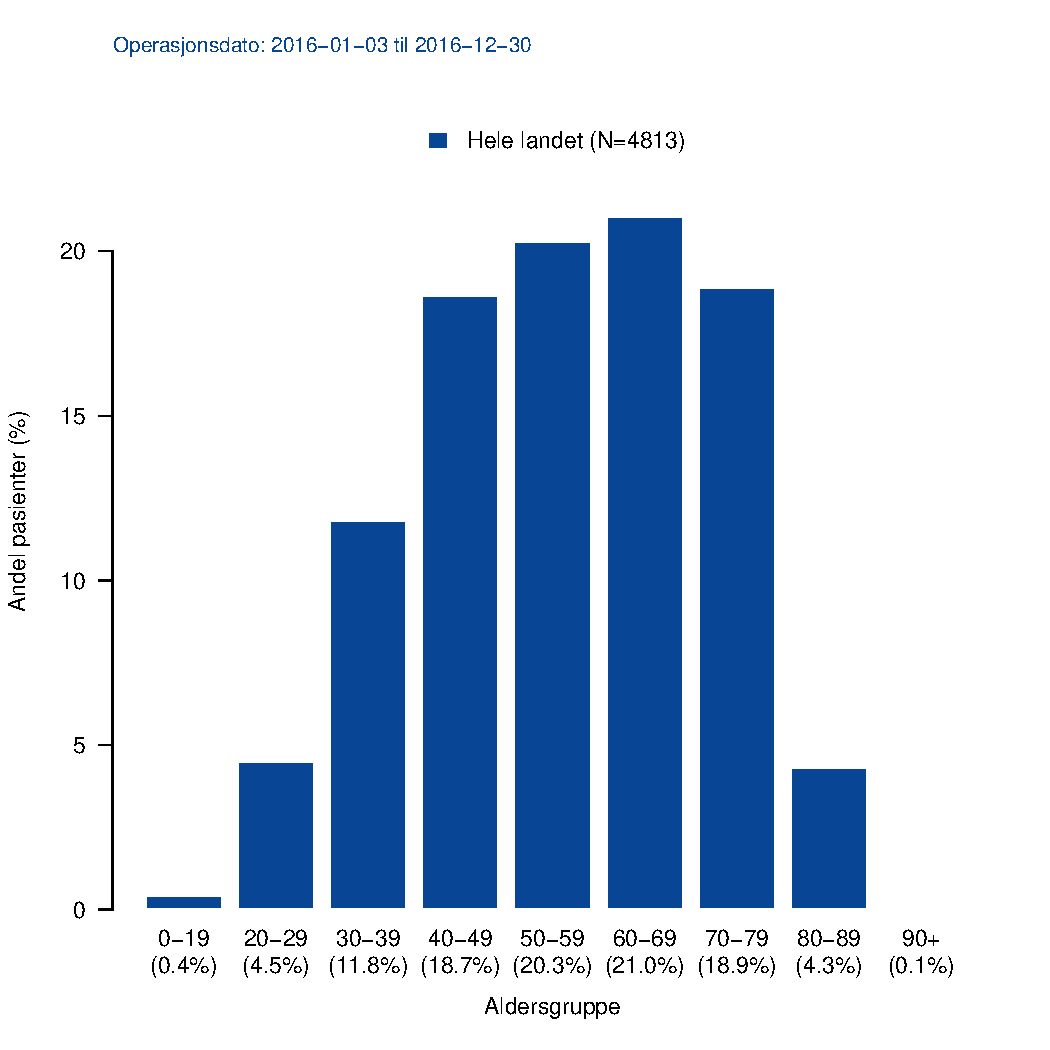
\includegraphics[width= s1\textwidth]{FigAlderFord.pdf}
%	\caption{\label{fig:Alder} paste0(AlderFord$Tittel,', ',rappAar)}
%\end{figure}

\subsection{Kroppsmasseindex (Body Mass Index, BMI)}



Opplysninger om høyde og vekt er rapportert fra pasientene selv.
Andelen pasienter med fedme har vært jevt økende fra 18.6 \%
til 24.5 \%
Figur \ref{fig:BMI} viser fordeling av BMI for alle pasienter i 2016. 

\begin{figure}[ht]
\scalebox{0.7}{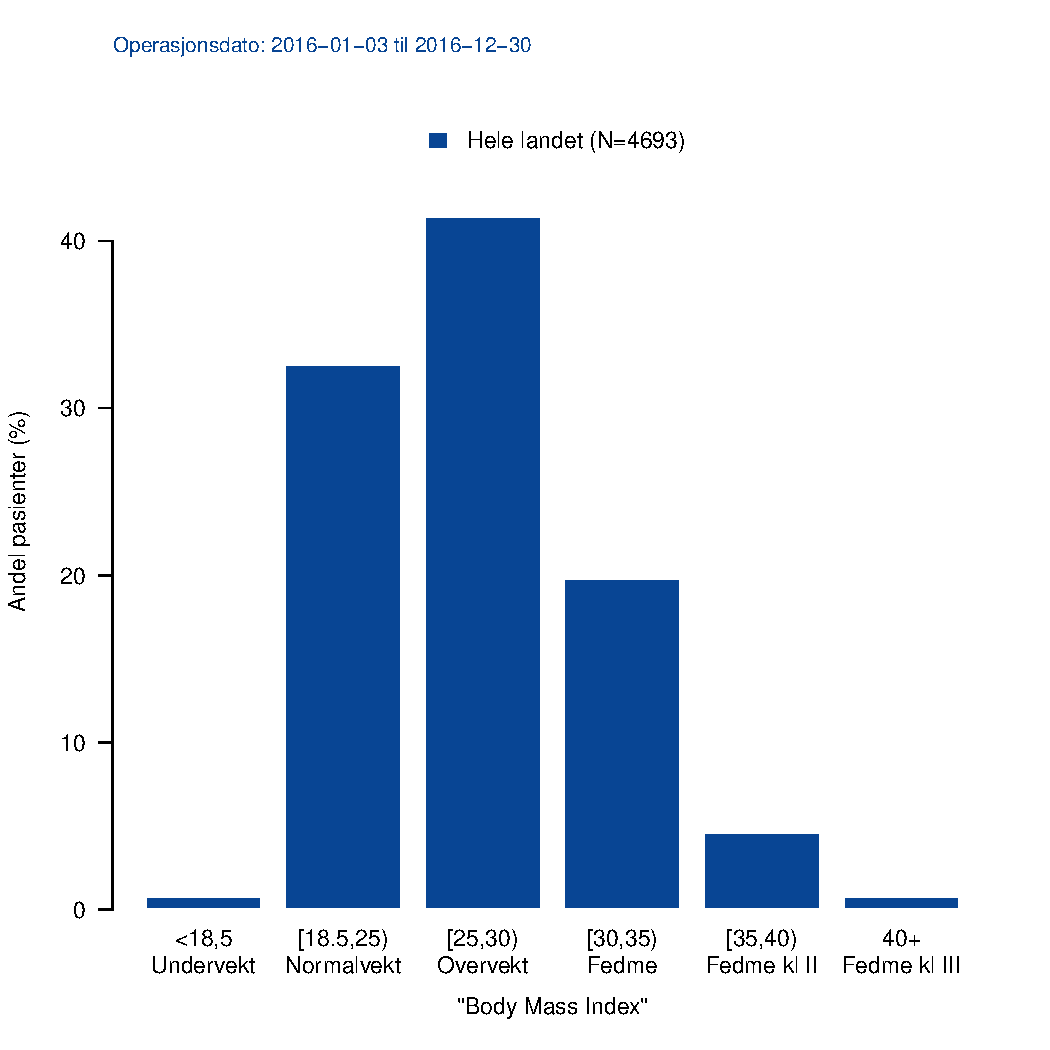
\includegraphics{Figurer/FigBMI.pdf}}
\caption{\label{fig:BMI} Pasientenes BMI (Body Mass Index).}
\end{figure}





\subsection{Morsmål / etnisitet og utdanning}

% latex table generated in R 3.4.1 by xtable 1.8-2 package
% Wed Sep 27 11:15:28 2017
\begin{table}[ht]
\centering
\begin{tabular}{lrr}
  \hline
 & Antall & Andeler \\ 
  \hline
Norsk & 4509 & 93.7\% \\ 
  Samisk & 5 & 0.1\% \\ 
  Annet & 277 & 5.8\% \\ 
  Ikke svart & 22 & 0.5\% \\ 
   \hline
\end{tabular}
\caption{Pasientenes morsmål} 
\label{tab:Morsm}
\end{table}


Tabell \ref{tab:Morsm} viser fordeling av norske, samiske og andre fremmedsåpråklige pasienter.
Andel fremmedspråklige pasienter (inkl. samisk) var 5.9\% . 

Andelen fremmedspråklige som opereres for prolaps har økt fra 5 \% til 7 \% i perioden.
Beslutning om ryggkirurgi baserer seg på en felles forståelse mellom kirurg og
pasient av hva helseproblemene består i og hva som kan oppnås med operasjon
(«shared desicion making»). I behandling av fremmedspråklige er kommunikasjon
en utfordring. Av de som har norsk som morsmål var suksessraten 65 \% mot 56 \%
for fremmedspråklige. Bedre kommunikasjon kan bidra å redusere disse
forskjellene. Figur \ref{fig:Morsmal} viser andelen fremmedspråklige operert ved de ulike avdelingene i 2016.

\begin{figure}[ht]
\scalebox{0.7}{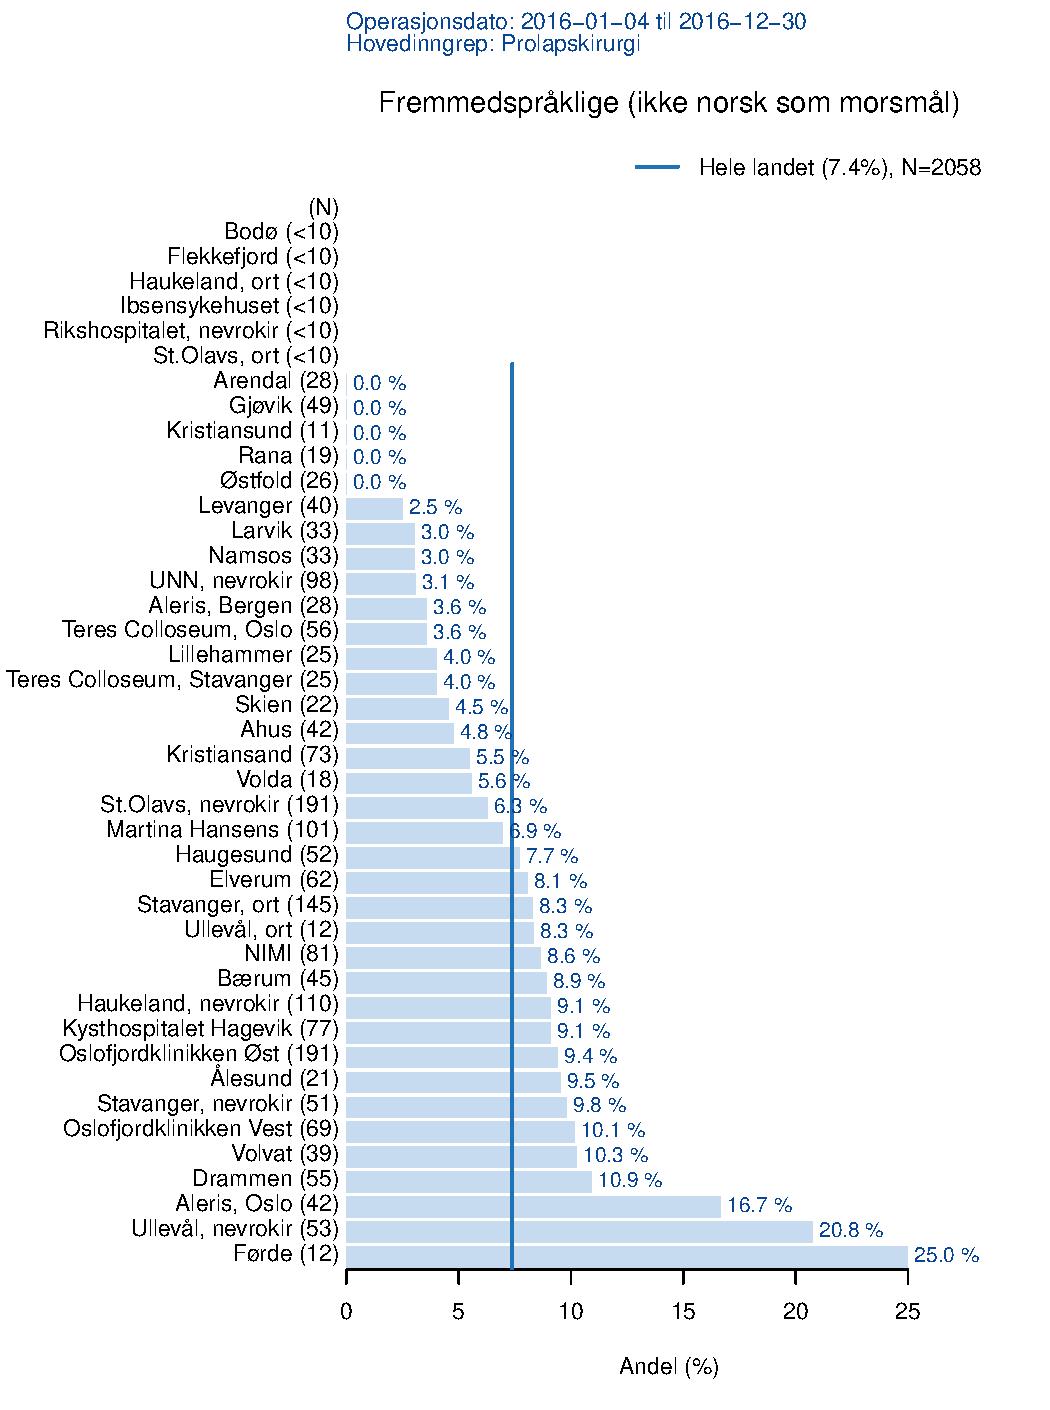
\includegraphics{Figurer/FigMorsmal.pdf}}
\caption{\label{fig:Morsmal} Andel fremmedspråklige av alle prolapsopererte ved ulike sykehus i
Norge.}
\end{figure}




Figur \ref{fig:Utd} viser nivå av utdanning og vi ser at det er 36.2, 0.0 som har høyere utdanning. Opplysningene om utdanning er rapportert av pasientene selv. 
Lav utdanning er assosiert til dårligere operasjonsresultat. Figur \ref{fig:HoyUtdAvd} viser andel pasienter med høyskole eller universistetsutdanning ved hvert sykehus/avdeling.

\begin{figure}[ht]
\scalebox{0.7}{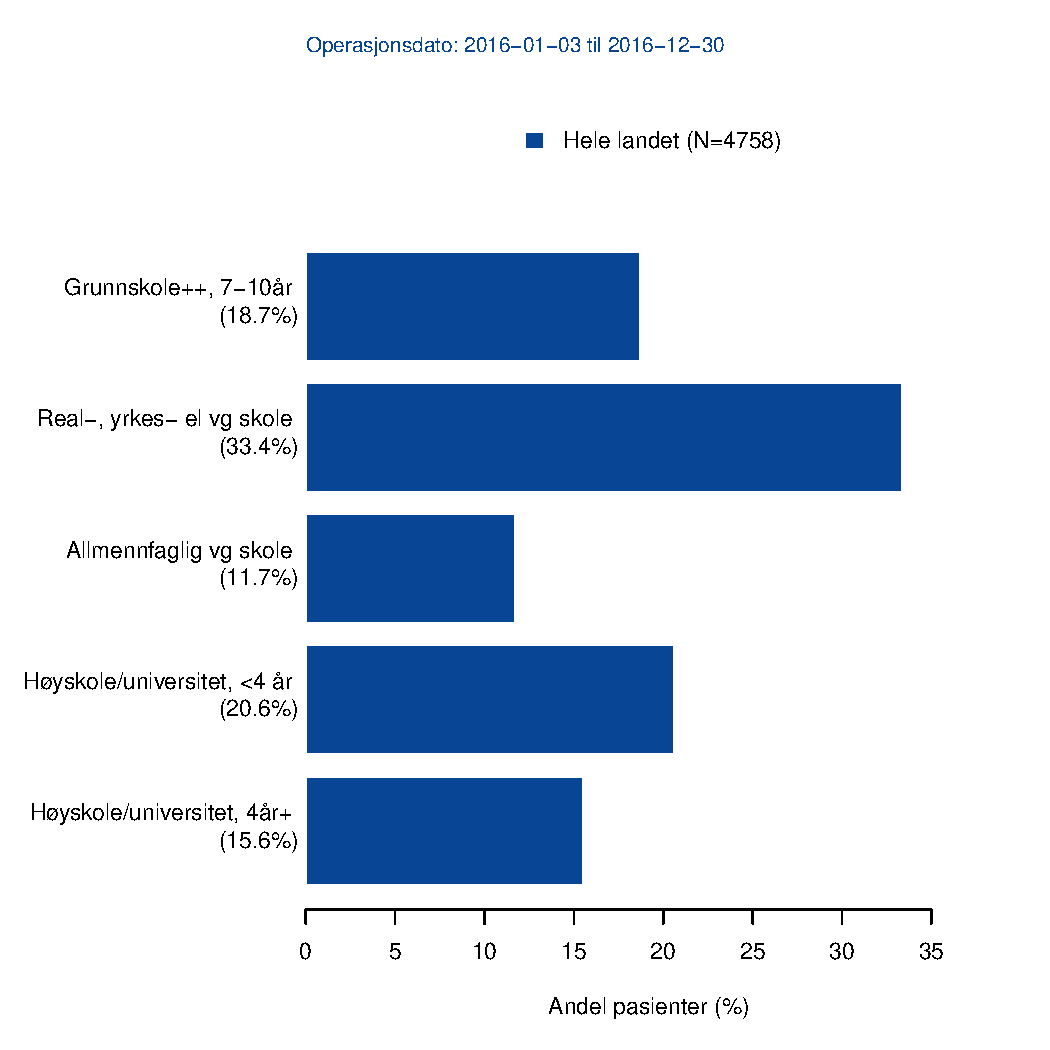
\includegraphics{Figurer/FigUtd.pdf}}
\caption{\label{fig:Utd} Høyeste fullførte utdanning.}
\end{figure}

\begin{figure}[ht]
\scalebox{0.7}{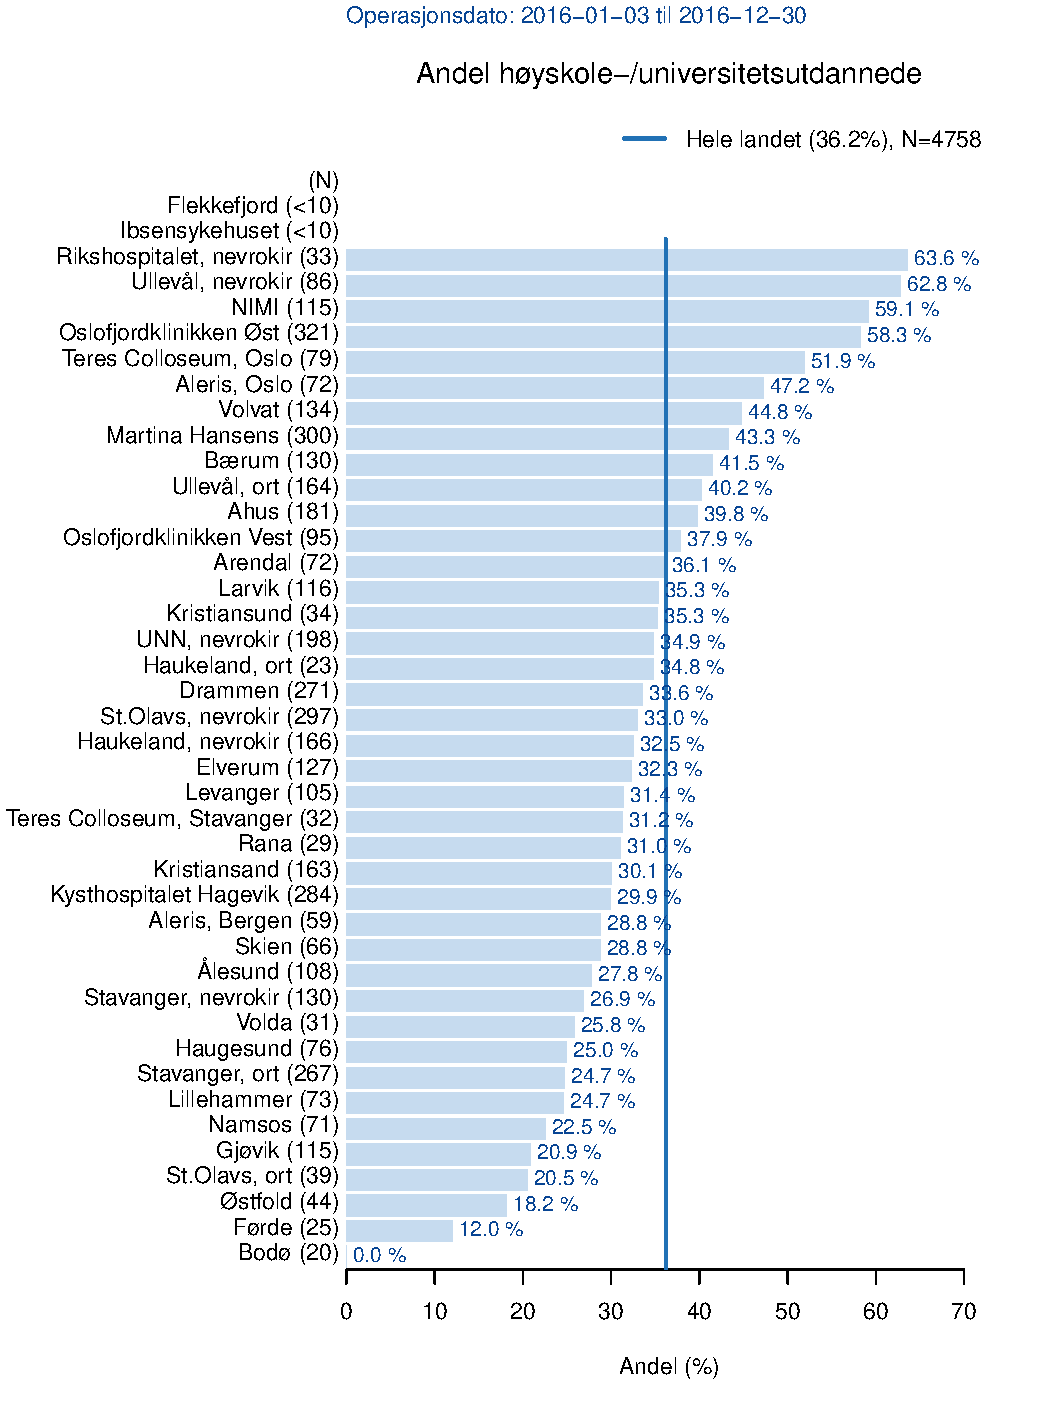
\includegraphics{Figurer/FigHoyUtdAvd.pdf}}
\caption{\label{fig:HoyUtdAvd} Andel pasienter med høyere utdanning.}
\end{figure}


\clearpage

\subsection{Arbeidsstatus}

% latex table generated in R 3.4.1 by xtable 1.8-2 package
% Wed Sep 27 11:15:29 2017
\begin{table}[ht]
\centering
\begin{tabular}{lr}
  \hline
 & Andeler \\ 
  \hline
I arbeid & 19.2\% \\ 
  Hjemmeværende & 1.6\% \\ 
  Student/skoleelev & 1.2\% \\ 
  Pensjonist & 28.8\% \\ 
  Arbeidsledig & 1.4\% \\ 
  Sykemeldt & 22.9\% \\ 
  Aktiv sykemeldt & 1.1\% \\ 
  Delvis Sykemeldt & 7.9\% \\ 
  Attføring/rehabiliteirng & 4.2\% \\ 
  Uføretrygdet & 11.6\% \\ 
   \hline
\end{tabular}
\caption{Arbeidsstatus, pasienter operert i 2016} 
\label{tab:Arb}
\end{table}


Tabell \ref{tab:Arb} viser fordeling av arbeidsstatus før operasjon for de 98.1\% 
av pasientene som har svart på spørsmål om arbeidsstatus.
Andelen pasienter som mottok sykepenger (sykemeldte, uføretrygdede eller personer 
på attføring) og av den grunn var helt eller delvis ute av jobb før operasjonen var 
47.7 \%. 
Median varighet av sykemelding/attføring/rehabilitering  før operasjon var 
15 uker.


%\clearpage


\subsection{Uføretrygd og erstatning }

Tabell \ref{tab:Ufor} viser pasientenes svar på spørsmålet: ``Har du søkt om uføretrygd?''.
Pasienter som har en uavklart uføre eller erstatningssak vil sjeldnere komme tidlig tilbake i jobb etter operasjon.
Andel som har søkt eller planlegger å søke uføretrygd ligger fortsatt stabilt like under 5 \% i 2016. 
Figur \ref{fig:Ufor} viser andel ryggopererte ved hver avdeling som har søkt eller planlegger å søke uføretrygd.

% latex table generated in R 3.4.1 by xtable 1.8-2 package
% Wed Sep 27 11:15:31 2017
\begin{table}[ht]
\centering
\begin{tabular}{lr}
  \hline
 & Andeler \\ 
  \hline
Ja & 2\% \\ 
  Nei & 75.2\% \\ 
  Planlegger å søke & 2.2\% \\ 
  Er innvilget & 11.5\% \\ 
  Ikke besvart & 9.1\% \\ 
   \hline
\end{tabular}
\caption{Spørsmål: Har du søkt om uføretrygd?} 
\label{tab:Ufor}
\end{table}


\begin{figure}[ht]
\scalebox{0.7}{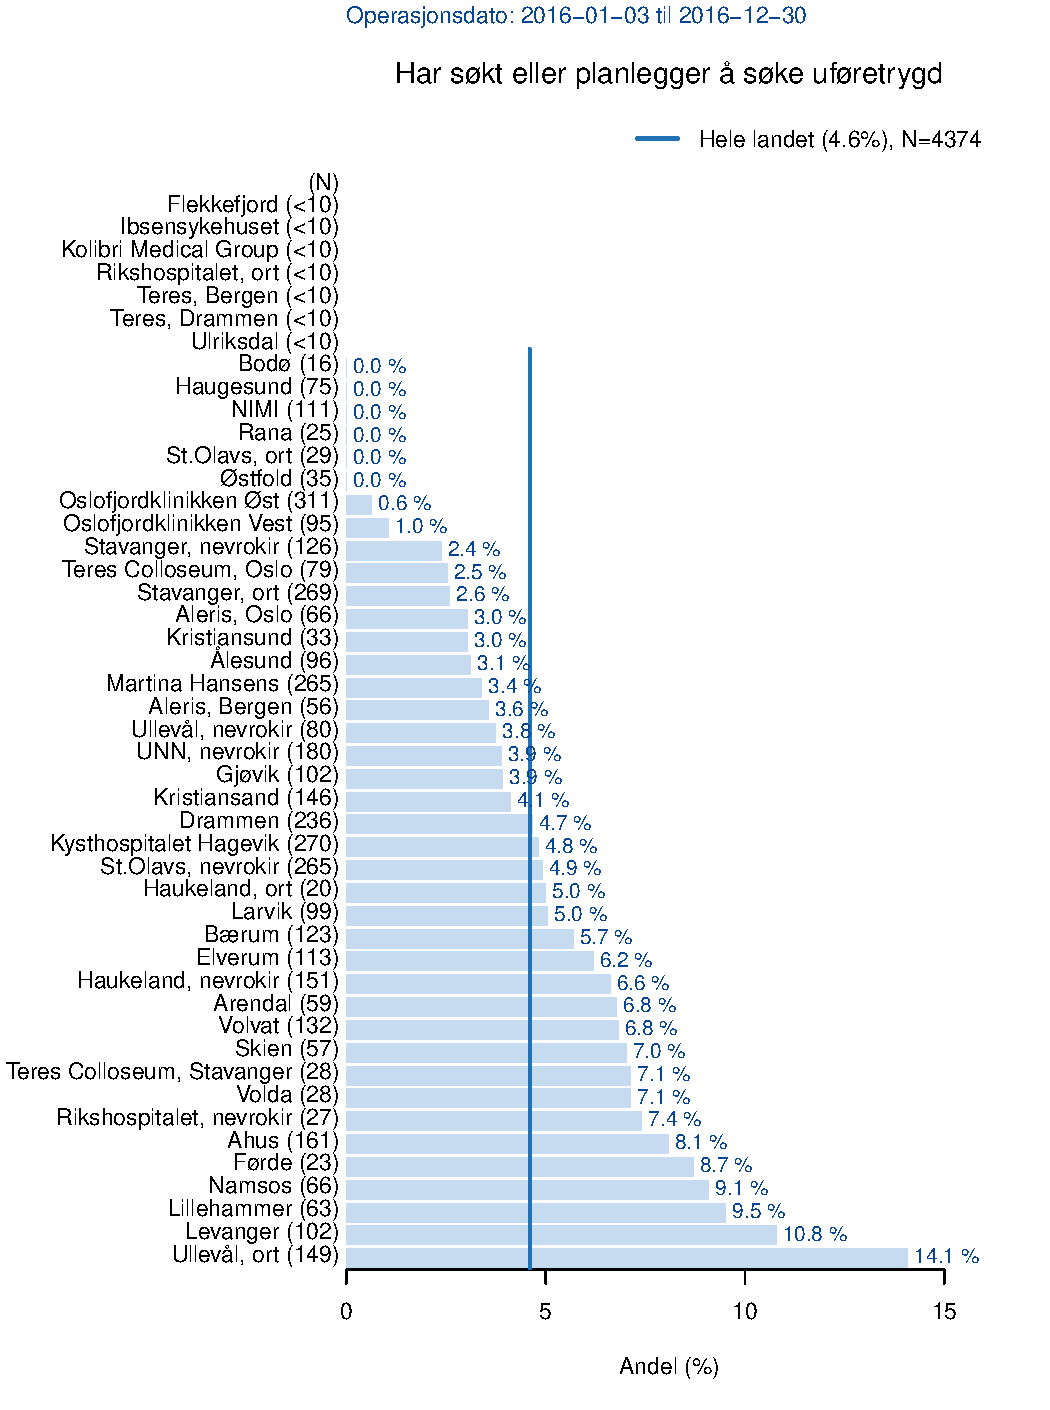
\includegraphics{Figurer/FigUforAvd.pdf}}
\caption{\label{fig:Ufor} Pasienter som har søkt eller planlegger å søke uføretrygd} 
\end{figure}

Tabell \ref{tab:Erst} viser pasientenes svar på spørsmålet: ``Har du søkt om erstatning?'' 

% latex table generated in R 3.4.1 by xtable 1.8-2 package
% Wed Sep 27 11:15:31 2017
\begin{table}[ht]
\centering
\begin{tabular}{lr}
  \hline
 & Andeler \\ 
  \hline
Ja & 2.6\% \\ 
  Nei & 87.6\% \\ 
  Planlegger å søke & 1.8\% \\ 
  Er innvilget & 2.1\% \\ 
  Ikke besvart & 5.9\% \\ 
   \hline
\end{tabular}
\caption{Spørsmål: Har du søkt om erstatning fra forsikringsselskap eller folketrygden, 
		eventuelt yrkesskadeerstatning)?} 
\label{tab:Erst}
\end{table}


\clearpage

\subsection{Tidligere ryggoperert}
Informasjonen er hentet fra legeskjema.
Figur \ref{fig:TidlOp} viser en prosentvis fordelig mellom primæroperasjon, det vil si første gangs 
operasjon, og operasjoner hos pasienter som har vært operert tidligere.  
Søylene representerer hvert år frem til i dag. Tallet på toppen av søylen viser antall operasjoner utført 
det aktuelle året. Reoperasjon gir genereltl dårligere operasjonsresultat enn første gangs operasjon.



\begin{figure}[ht]
\scalebox{0.7}{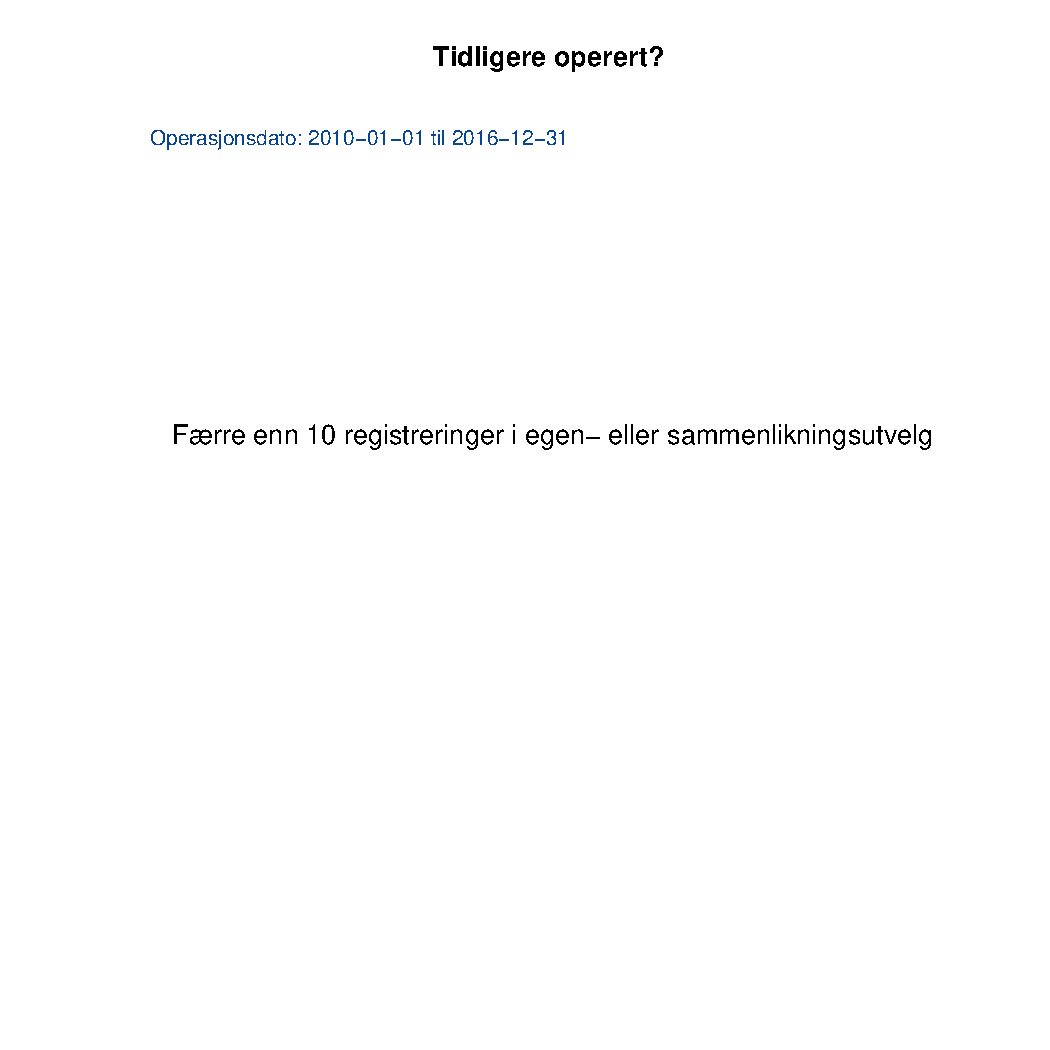
\includegraphics{Figurer/TidlOp.pdf}}
\caption{\label{fig:TidlOp} Tidligere operert? }
\end{figure}



Av de pasientene operert i 2016 som hadde vært operert tidligere, var 61.1\% 
operert i samme nivå, 33.5\% 
operert i annet nivå og 5.4\% 
operert i både samme og annet nivå.
Andelen reoperasjoner var 25 \% i 2010 og 27 \% i 2016.



\subsection{Varighet av smerter i rygg-/hofte og av utstrålende smerter på operasjonstidspunktet}

% latex table generated in R 3.4.1 by xtable 1.8-2 package
% Wed Sep 27 11:15:33 2017
\begin{table}[ht]
\centering
\begin{tabular}{lr}
  \hline
 & Andeler \\ 
  \hline
Ingen rygg-/hoftesmerter & 1.7\% \\ 
  $<$ 3 mnd & 9\% \\ 
  3 - 12 mnd & 30.8\% \\ 
  1 - 2 år & 16.5\% \\ 
  $>$ 2 år & 38.2\% \\ 
  Ikke besvart & 3.8\% \\ 
   \hline
\end{tabular}
\caption{Varighet av rygg-/hoftesmerter på operasjonstidspunktet} 
\label{tab:SmRH}
\end{table}
% latex table generated in R 3.4.1 by xtable 1.8-2 package
% Wed Sep 27 11:15:33 2017
\begin{table}[ht]
\centering
\begin{tabular}{lr}
  \hline
 & Andeler \\ 
  \hline
Ingen utstrålende smerter & 2.7\% \\ 
  $<$ 3 mnd & 13.5\% \\ 
  3 - 12 mnd & 35\% \\ 
  1 - 2 år & 17.5\% \\ 
  $>$ 2 år & 26.2\% \\ 
  Ikke besvart & 5.2\% \\ 
   \hline
\end{tabular}
\caption{Varighet av nåværende utstrålende smerter} 
\label{tab:Utstr}
\end{table}

I nasjonale retningslinjer (2007) er det anbefalt å operere pasienter for prolaps før
beinsmertene har vart for lenge, helst innen ett år. Derfor bør
pasientgruppen håndteres raskt og effektivt når beslutning om operasjon er tatt og
ikke-kirurgisk behandling har vært forsøkt. Data fra NKR og nyere forskning viser at
pasienter som opereres for prolaps og har hatt beinsmerter mer enn ett år har
dårligere prognose. Andelen pasienter med beinsmerter mer enn ett år på
operasjonstidspunkt var uendret fra 2010 til 2016 (47\%).
Figur 7 viser at det er stor variasjon i varighet av beinsmerter hos pasienter som blir
operert ved ulike sykehus. Det har sannsynligvis sammenheng med ventetid for
utredning og operasjon og tilgjengelig operasjonskapasitet i forhold til etterspørsel.

Tabellene \ref{tab:SmRH}  og \ref{tab:Utstr} viser fordeling av hvor lenge pasientene har hatt 
hhv. smerter i rygg/hofte og utstrålende smerter. 
Figurene \ref{fig:VarighSmerteUtstrAvdPro} og \ref{fig:VarighSmerteUtstrAvdSS} viser hvor stor andel av henholdsvis prolaps- og spinal stenosepasienter som har hatt ustrålende smerter i mer enn ett år ved hvert sykehus. 
Figurene \ref{fig:VarighSmerteRyggAvdPro} og \ref{fig:VarighSmerteRyggAvdSS} viser hvor stor andel av henholdsvis prolaps- og spinal stenosepasienter som har hatt rygg-/hoftesmerter mer enn ett år ved hvert sykehus.

\begin{figure}[h] 
\scalebox{0.7}{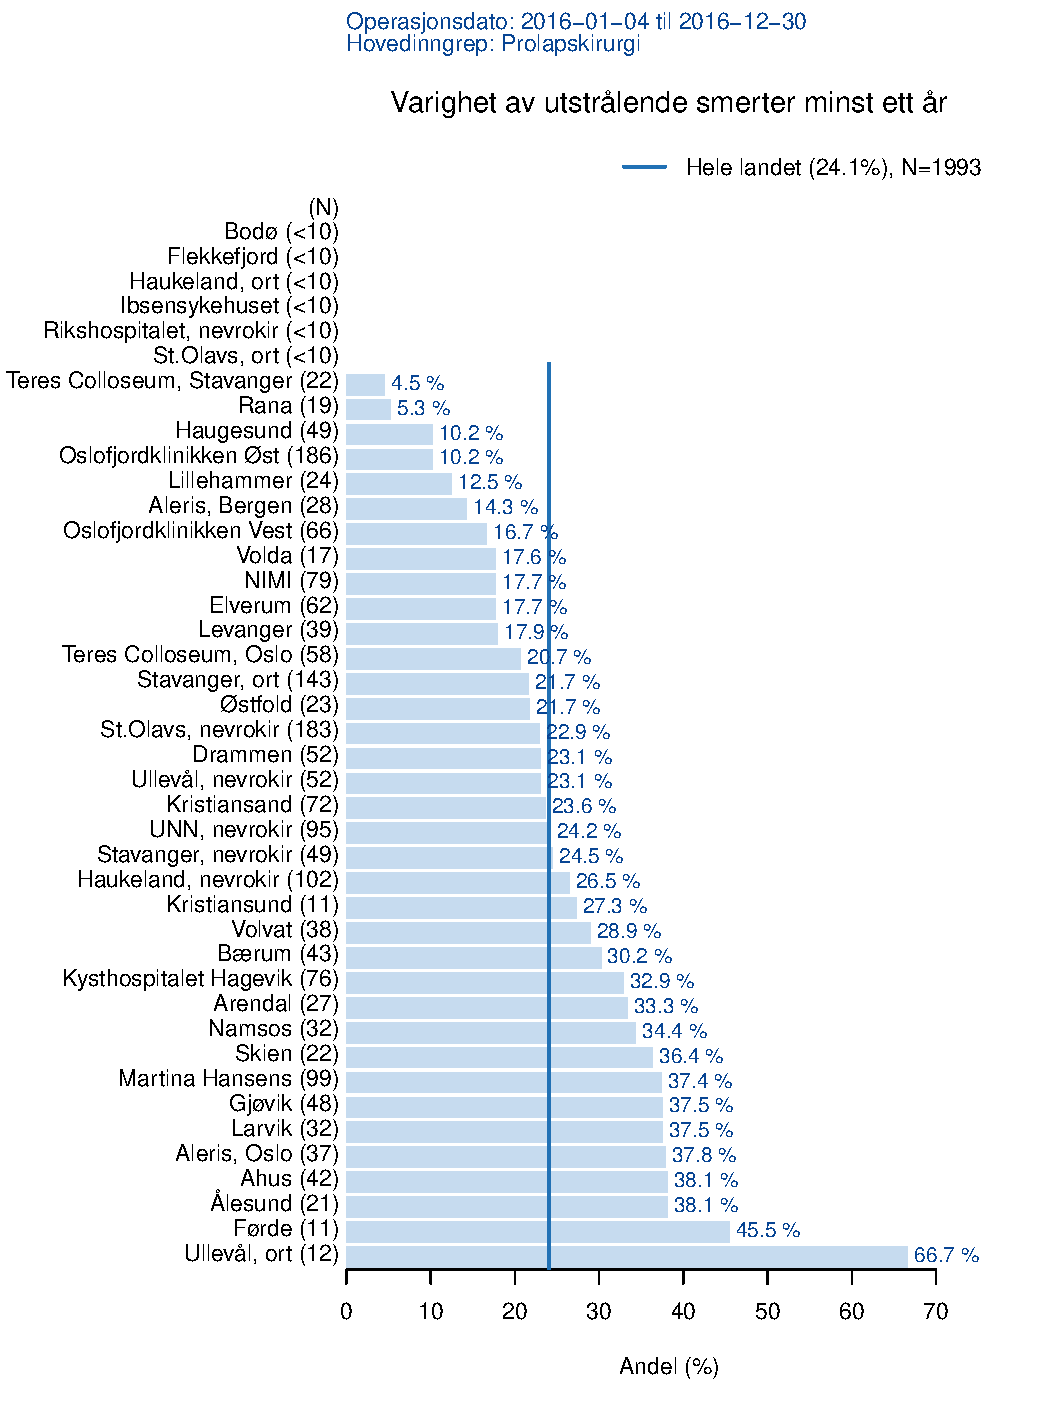
\includegraphics{Figurer/VarighUtstrAvdPro.pdf}}
\caption{Prolapspasienter som har utstrålende smerter i mer enn ett år før operasjonen.}
\label{fig:VarighSmerteUtstrAvdPro}
\end{figure}

\begin{figure}[h] 
\scalebox{0.7}{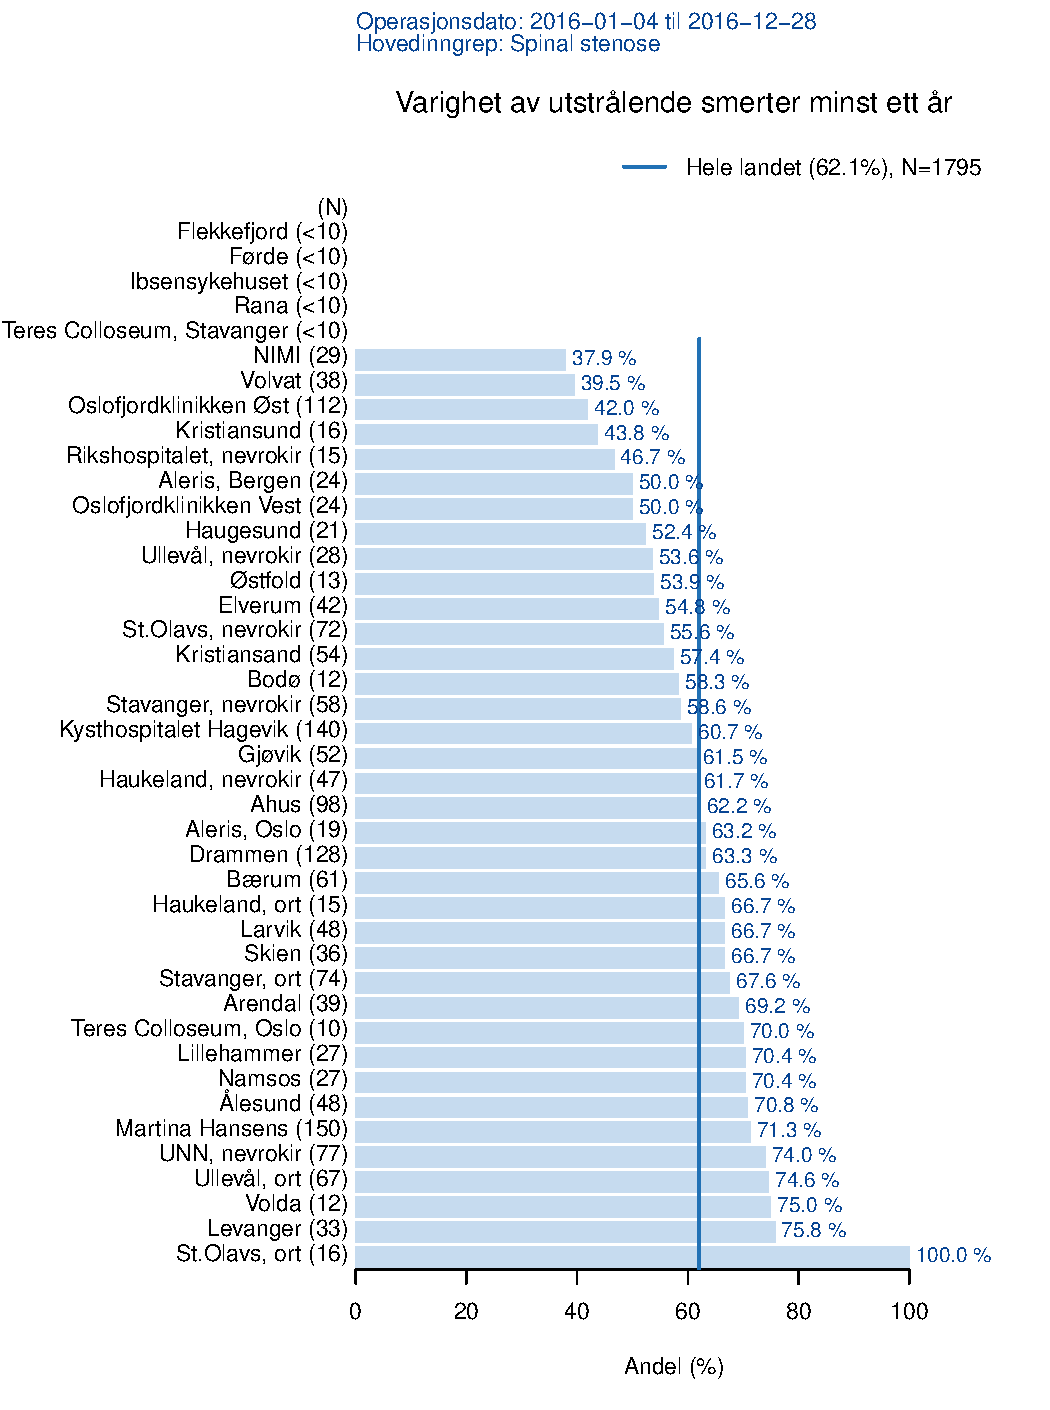
\includegraphics{Figurer/VarighUtstrAvdSS.pdf}}
\caption{Spinal stenosepasienter som har utstrålende smerter i mer enn ett år før operasjonen.}
\label{fig:VarighSmerteUtstrAvdSS}
\end{figure}

Figur \ref{fig:VarighSmerteUtstrTid} viser utvikling over tid for andel pasienter med lang symptomvarighet. 

\begin{figure}[h] 
\center{
\scalebox{0.55}{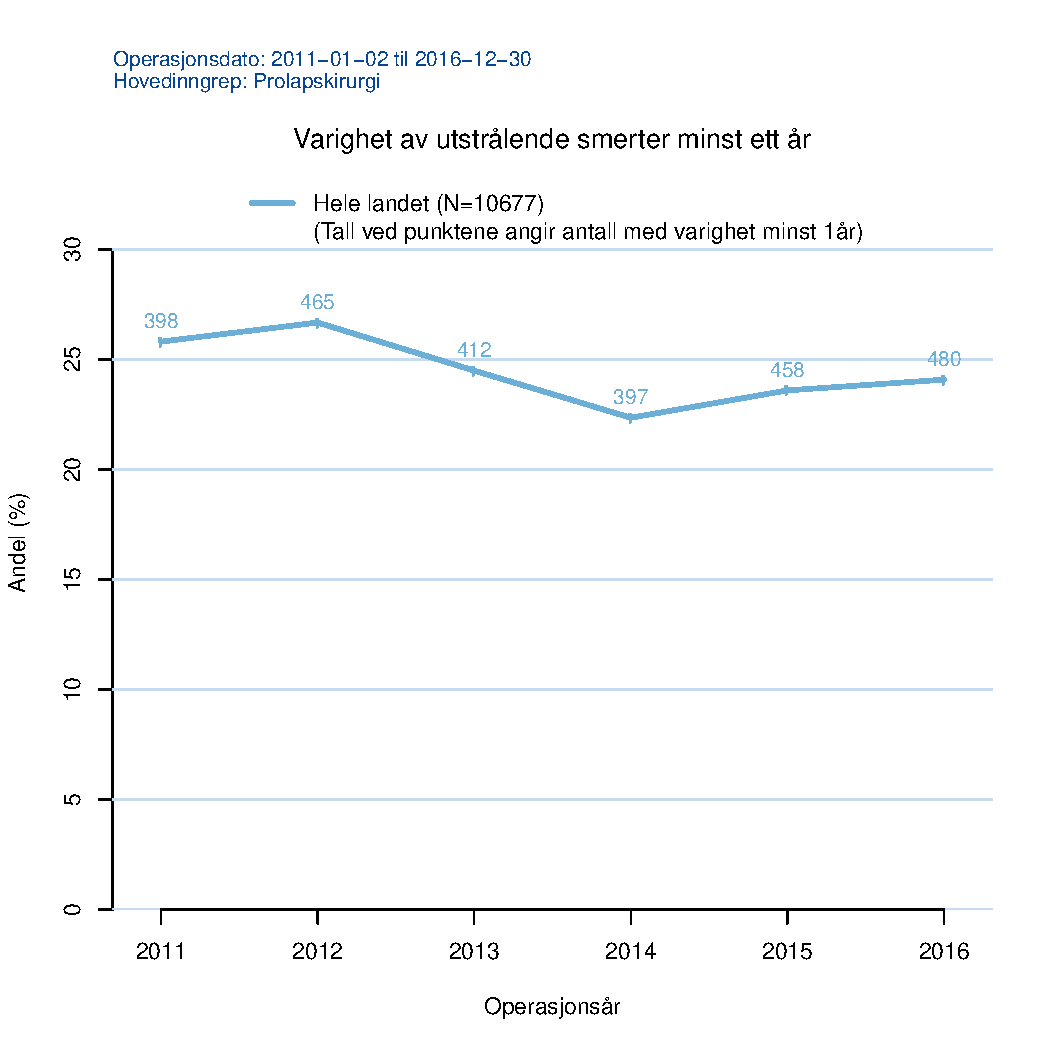
\includegraphics{Figurer/VarighUtstrTidPro.pdf}}
\scalebox{0.55}{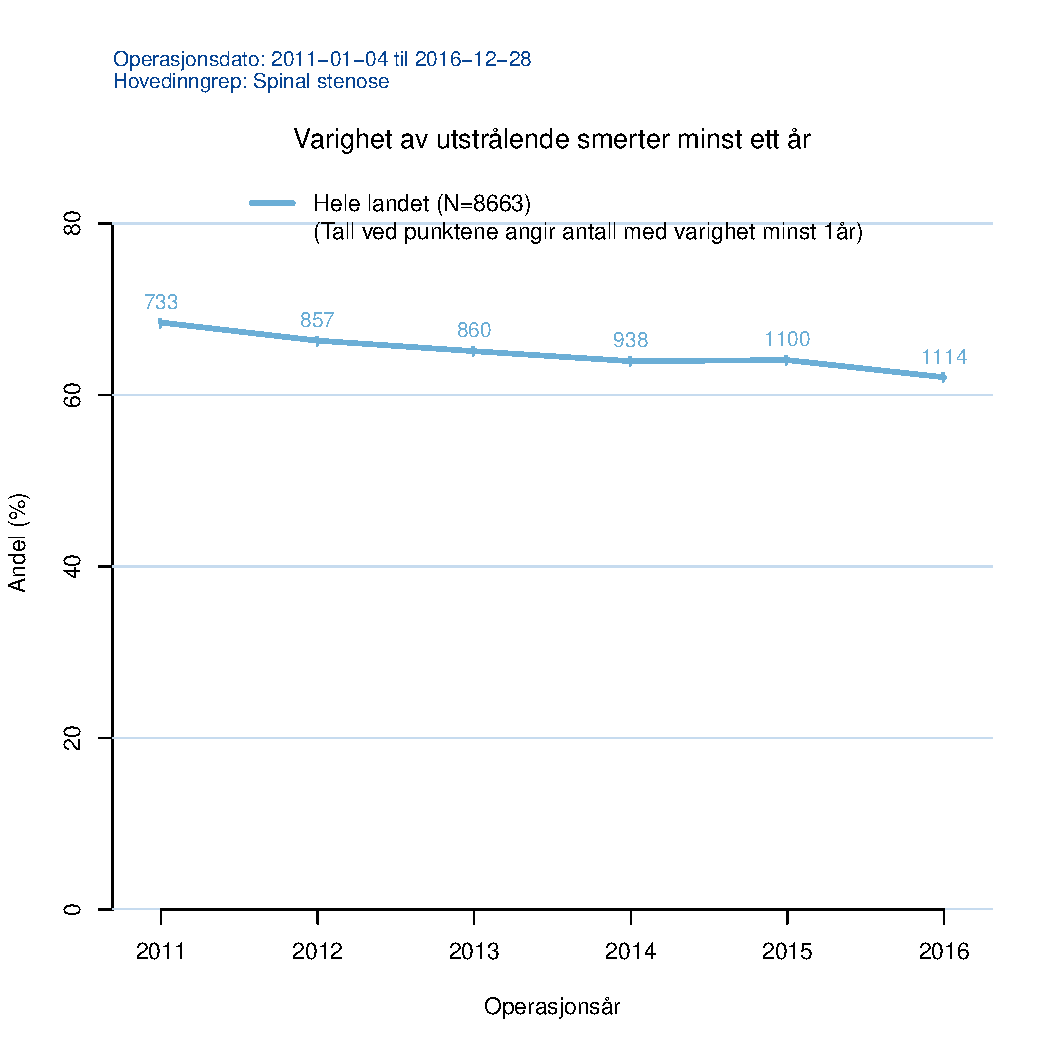
\includegraphics{Figurer/VarighUtstrTidSS.pdf}}} 
\caption{Prolaps- og Spinal stenosepasienter som har utstrålende smerter i mer enn ett år før operasjonen, utvikling over tid.}
\label{fig:VarighSmerteUtstrTid}
\end{figure}



\begin{figure}[h] 
\scalebox{0.7}{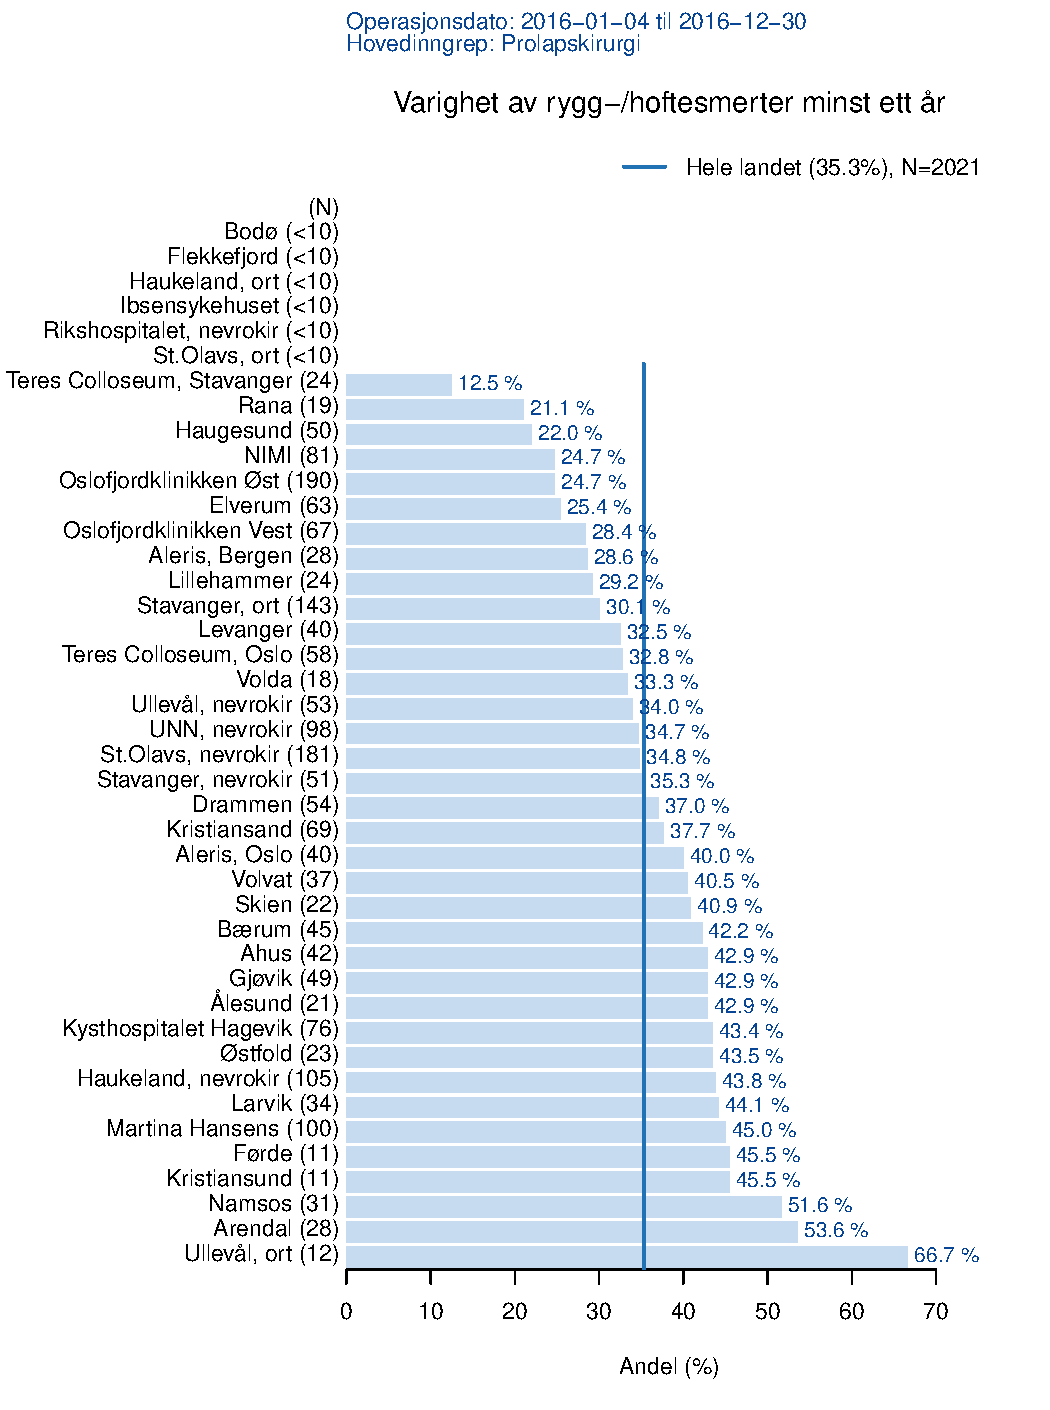
\includegraphics{Figurer/VarighRyggHofAvdPro.pdf}}
\caption{Prolapspasienter som har hatt smerter i rygg-/hofte
i mer enn ett år før operasjonen.}
\label{fig:VarighSmerteRyggAvdPro}
\end{figure}

\begin{figure}[h] 
\scalebox{0.7}{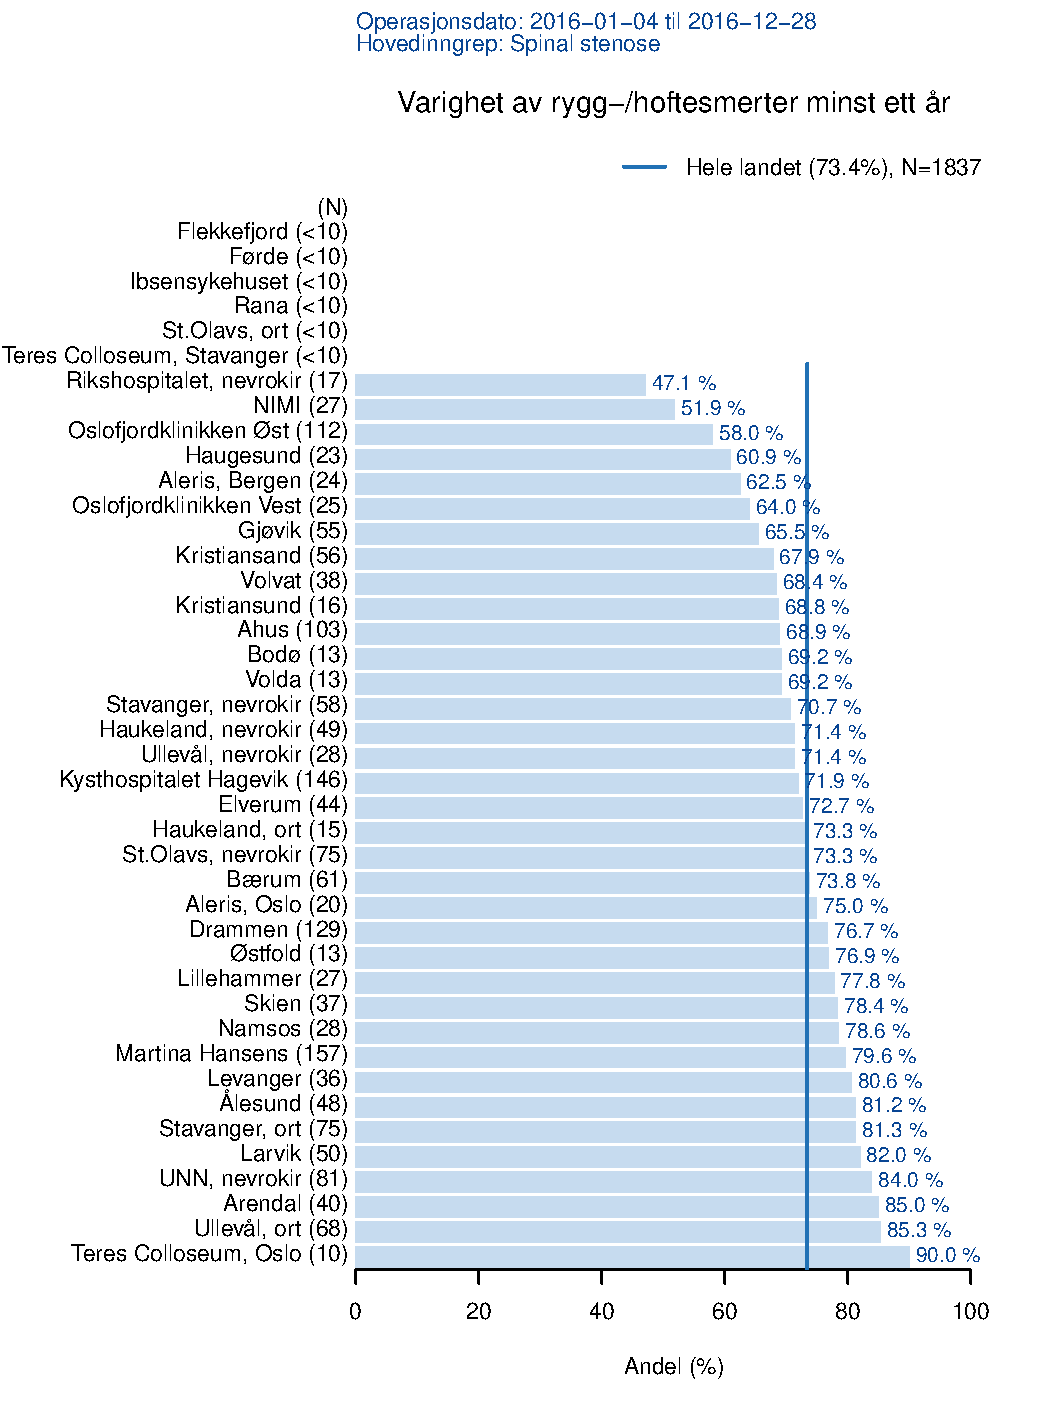
\includegraphics{Figurer/VarighRyggHofAvdSS.pdf}}
\caption{Spinal stenosepasienter som har hatt smerter i rygg-/hofte
i mer enn ett år før operasjonen.}
\label{fig:VarighSmerteRyggAvdSS}
\end{figure}




\clearpage



\subsection{ASA-grad og røyking}
ASA angir pasientens ”sårbarhet” i forhold til å få anestesi og operasjon på en skala fra 1 til 5. 
Opplysningene skal hentes fra anestesiskjema som fylles ut av anestesilege/sykepleier før operasjon.
% latex table generated in R 3.4.1 by xtable 1.8-2 package
% Wed Sep 27 11:15:36 2017
\begin{table}[ht]
\centering
\begin{tabular}{crr}
  \hline
 & Antall & Prosent \\ 
  \hline
I & 1334 & 27.7\% \\ 
  II & 2787 & 57.9\% \\ 
  III & 657 & 13.7\% \\ 
  IV & 5 & 0.1\% \\ 
  Ikke besvart & 30 & 0.6\% \\ 
   \hline
\end{tabular}
\caption{Fordeling av ASA-grad, operasjoner utført i 2016} 
\label{tab:ASA}
\end{table}


Tabell \ref{tab:ASA} viser fordeling av ASA grad. Andelen pasienter med ASA grad I-II 
var 85.6\%. Pasienter som røyker, havner automatisk i ASA-grad II eller høyere. 
Det er 21\% av mennene og 22\% av kvinnene som røyker. 
                    Total andel røykere er 21\%



\subsection{Radiologisk utredning}

% latex table generated in R 3.4.1 by xtable 1.8-2 package
% Wed Sep 27 11:15:36 2017
\begin{table}[ht]
\centering
\begin{tabular}{lrr}
  \hline
 & Antall & Andeler \\ 
  \hline
CT & 339 & 7\% \\ 
  MR & 4712 & 98\% \\ 
  Radikulografi & 33 & 1\% \\ 
  Diskografi & 2 & 0\% \\ 
  Diagnostisk blokade & 12 & 0\% \\ 
  Røntgen LS-columna & 1043 & 22\% \\ 
  Med fleksjon/ekstensjon & 335 & 7\% \\ 
  Tot. ant. & 4813 &   \\ 
   \hline
\end{tabular}
\caption{Radiologisk vurdering, 2016} 
\label{tab:RV}
\end{table}


Tabell \ref{tab:RV} viser hvor stor andel av pasientene som har vært til ulike typer 
radiologisk undersøkelse. Hyppigste årsak til operasjon (indikasjon) er skiveprolaps og spinal stenose eller kombinasjoner av disse tilstandene.
Spørsmålene er besvart av leger. En pasient kan ha vært til flere undersøkelser.




% latex table generated in R 3.4.1 by xtable 1.8-2 package
% Wed Sep 27 11:15:36 2017
\begin{table}[ht]
\centering
\begin{tabular}{lrr}
  \hline
 & Antall & Andeler \\ 
  \hline
Skiveprolaps & 2206 & 46\% \\ 
  Sentral spinalstenose & 1498 & 31\% \\ 
  Lateral spinalstenose & 1578 & 33\% \\ 
  Foraminal stenose & 590 & 12\% \\ 
  Degenerativ rygg/skivedegenerasjon & 767 & 16\% \\ 
  Istmisk spondylolistese & 146 & 3\% \\ 
  Degenerativ spondylolistese & 414 & 9\% \\ 
  Degenerativ skoliose & 125 & 3\% \\ 
  Synovial syste & 92 & 2\% \\ 
  Pseudomeningocele & 1 & 0\% \\ 
  Tot.ant. & 4813 &   \\ 
   \hline
\end{tabular}
\caption{Radiologiske diagnoser, 2016} 
\label{tab:RF}
\end{table}


Tabell \ref{tab:RF} viser diagnoser basert på radiologiske funn hos alle pasienter 
i 2016. 
Spørsmålene er besvart av leger.
En pasient kan ha flere diagnoser/radiologiske funn.
``Normalt'' er registrert som eneste billedfunn hos 1 pasient(er).
                                  ``Normal'' kan ikke være eneste billedfunn, så eventuelle registreringer skyldes sannsynligvis 
                                  feil/unøyaktig registrering.




\section{Virksomhetsdata}

\subsection{Type operasjon}



De hyppigste tilstandene pasienter opereres for er prolapskirurgi (43 \%) og spinal stenose (40 \%). Tabell \ref{tab:AntHovedInngrep} viser fordeling av hovedinngrepstype, samt antall registrerte operasjoner for hver hovedinngrepstype.

% latex table generated in R 3.4.1 by xtable 1.8-2 package
% Wed Sep 27 11:15:36 2017
\begin{table}[ht]
\centering
\begin{tabular}{lrr}
  \hline
 & Antall & Andeler \\ 
  \hline
Udefinerbart & 127 & 3\% \\ 
  Prolapskirurgi & 2065 & 43\% \\ 
  Foramenotomi & 1816 & 38\% \\ 
  Laminektomi & 196 & 4\% \\ 
  Interspin. implantat & 0 & 0\% \\ 
  Fusjonskirurgi & 545 & 11\% \\ 
  Skiveprotese & 32 & 1\% \\ 
  Rev. av implantat & 32 & 1\% \\ 
   \hline
\end{tabular}
\caption{Fordeling av hovedinngrep, 2016} 
\label{tab:AntHovedInngrep}
\end{table}



%\begin{figure}[ht]
%      \scalebox{s1}{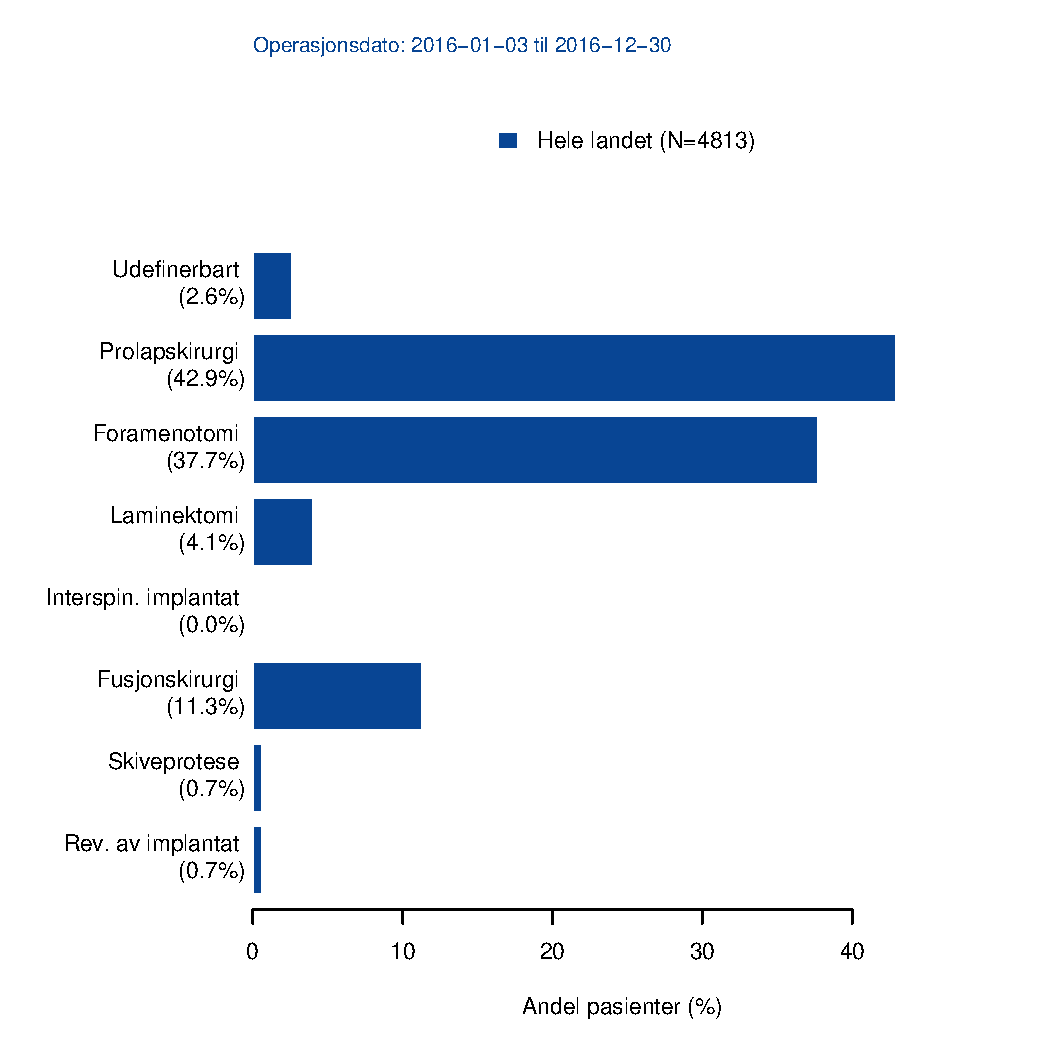
\includegraphics{Figurer/HovedInngrep.pdf}}
%      \caption{\label{fig:HovedInngrep} HovedInngrep$Tittel}
%\end{figure}



\subsubsection{Degen. spondylolistese operert med fusjonskirurgi}


En andel av de som har spinal stenose har også en forskyvning mellom ryggvirvlene (Degenerativ spondylolistese). I faglitteraturen er det sprikende anbefalinger for om denne undergruppen skal ha tilleggsbehandling med avstivningsoperasjon (fusjonskirurgi).
Figur \ref{fig:degSponFusj} viser at det er stor variasjon i bruk av denne fusjonskirurgi i Norge. Det pågår flere forskningstudier for å kartlegge om denne tilleggsbehandlingen er nødvendig. 



\begin{figure}[ht]
\scalebox{0.7}{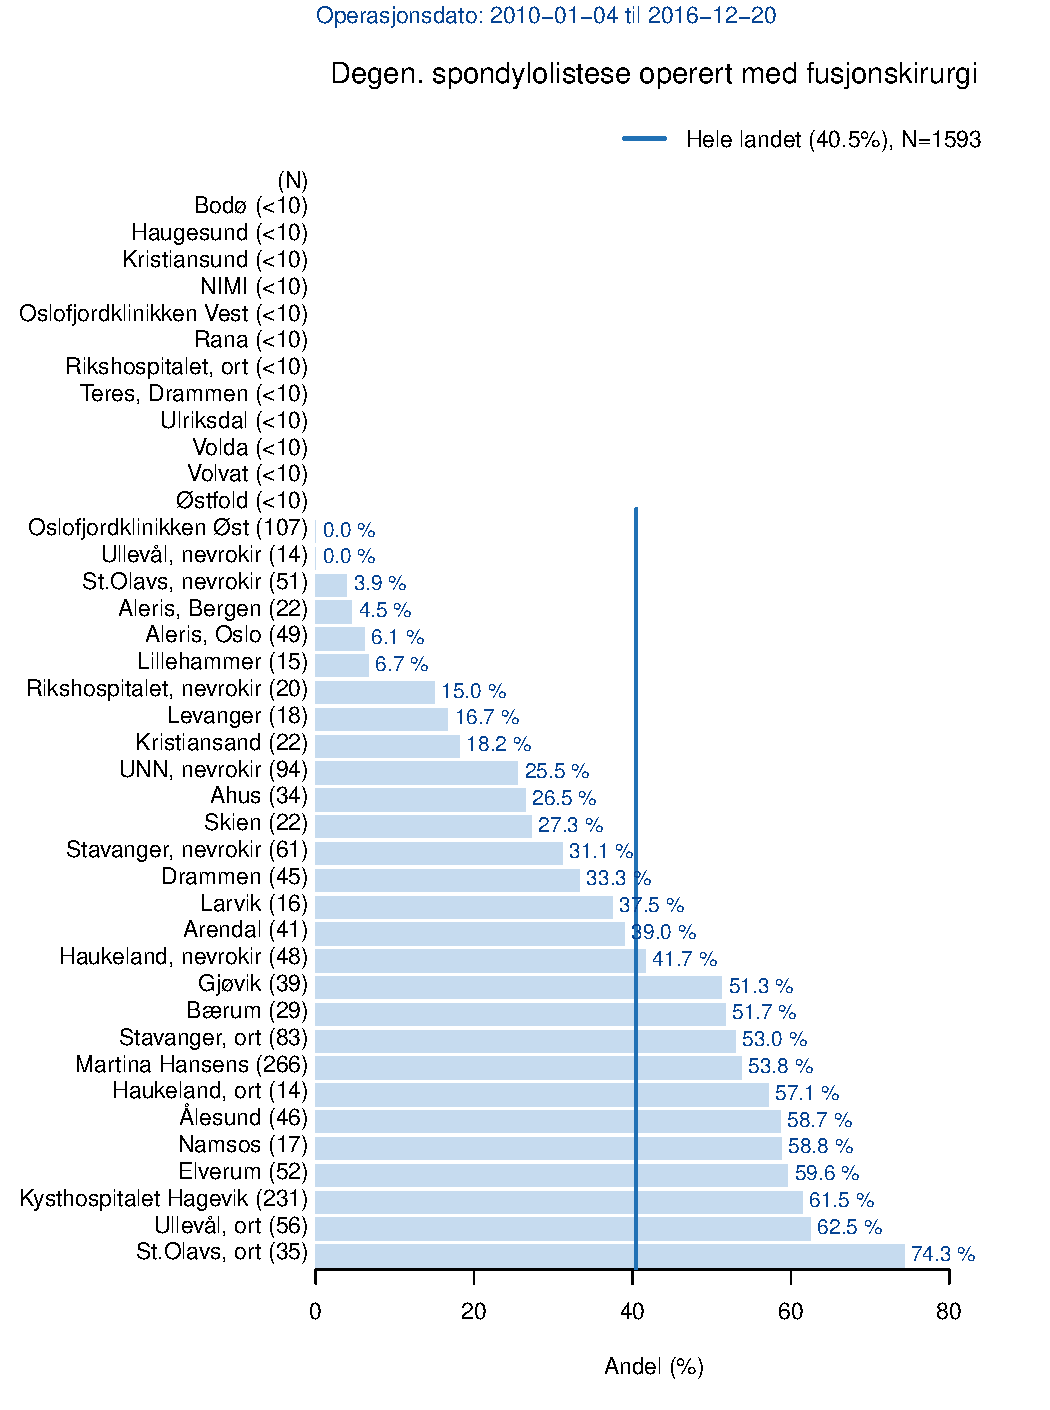
\includegraphics{Figurer/FigdegSponFusj.pdf}}
\caption{\label{fig:degSponFusj} Degenerativ spondylolistese operert med fusjonskirurgi}
\end{figure}


\clearpage

\subsection{Liggetid}

Informasjonen er hentet fra legeskjema.
Figur \ref{fig:Liggedogn} viser liggedøgnsfordeling for alle pasienter operert i 2016. Figur \ref{fig:LiggedognTid} viser gjennomsnittlig antall liggedøgn per år.  
Figur \ref{fig:LiggetidAvdPro} og \ref{fig:LiggetidAvdSS} viser at det er stor variasjon i antall liggedøgn mellom sykehus og avdelinger.
Det har vært en klar reduksjon i  liggetid på sykehus  for både prolaps og spinal stenose opererte (ca 1 døgn). Dette henger sammen med økt bruk av mindre invassive operasjonsmetoder og dermed mer dagkirurgi. 





\begin{figure}[h] 
\scalebox{0.7}{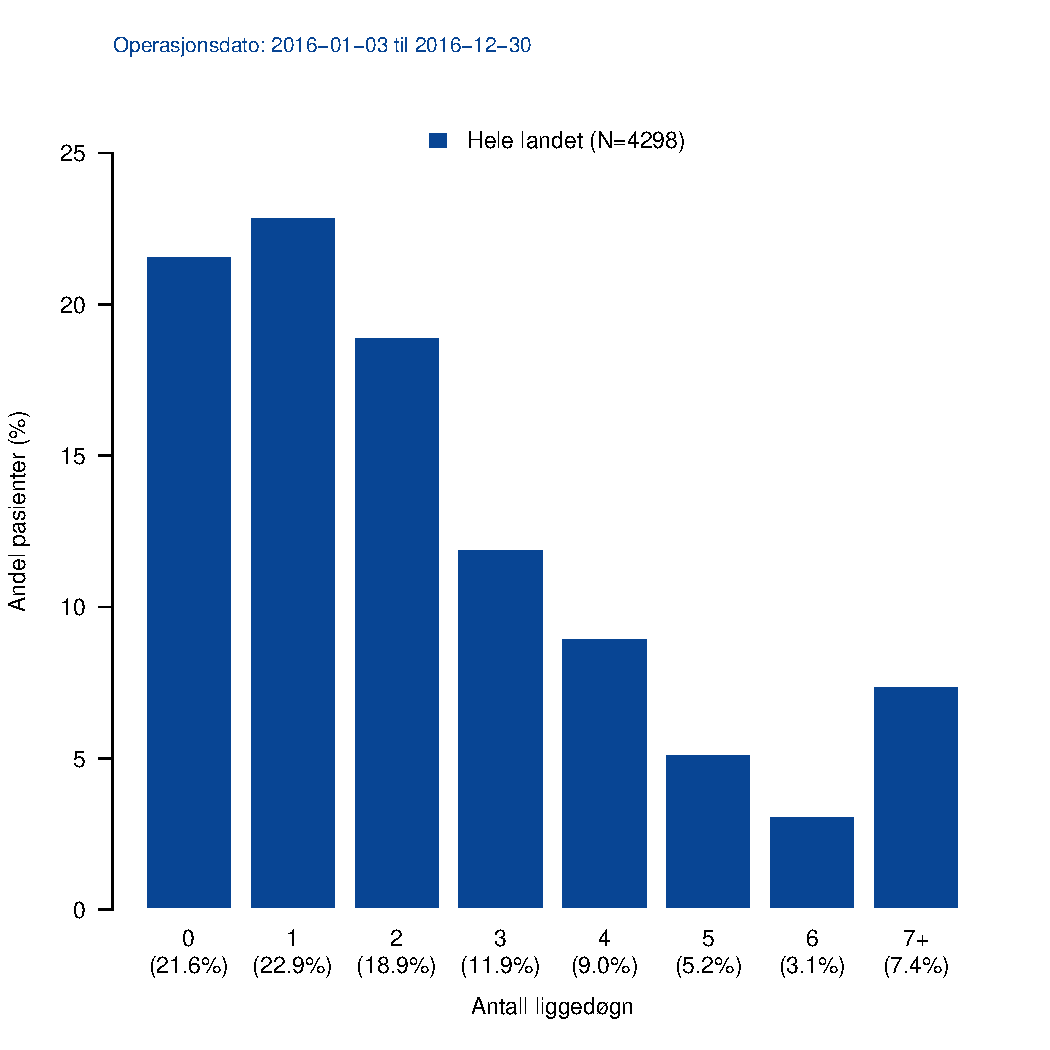
\includegraphics{Figurer/FigLiggetidFord.pdf}}
\caption{Liggetid ved operasjon.}
\label{fig:Liggedogn}
\end{figure}

\begin{figure}[h] 
\centerline{
\scalebox{0.55}{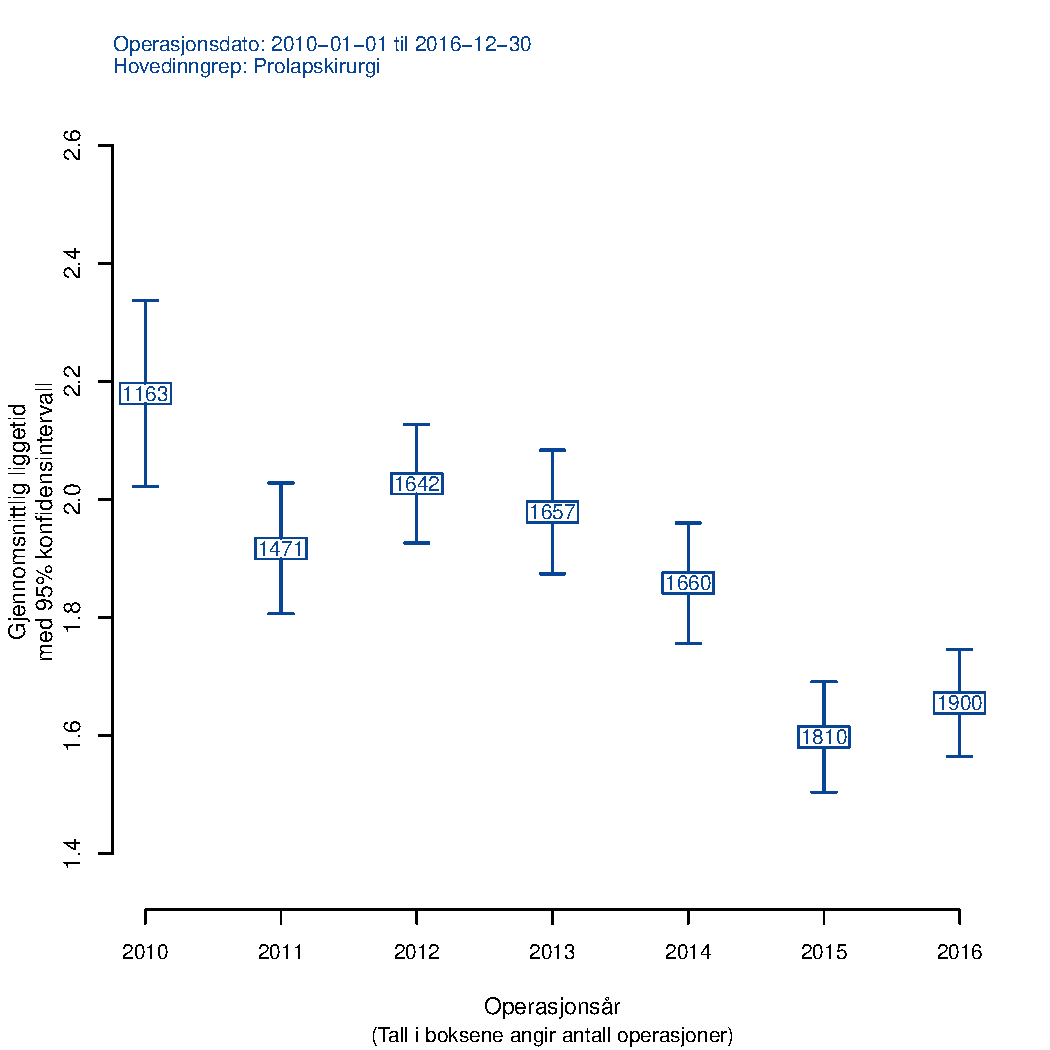
\includegraphics{Figurer/LiggetidBoxPro.pdf}}
\scalebox{0.55}{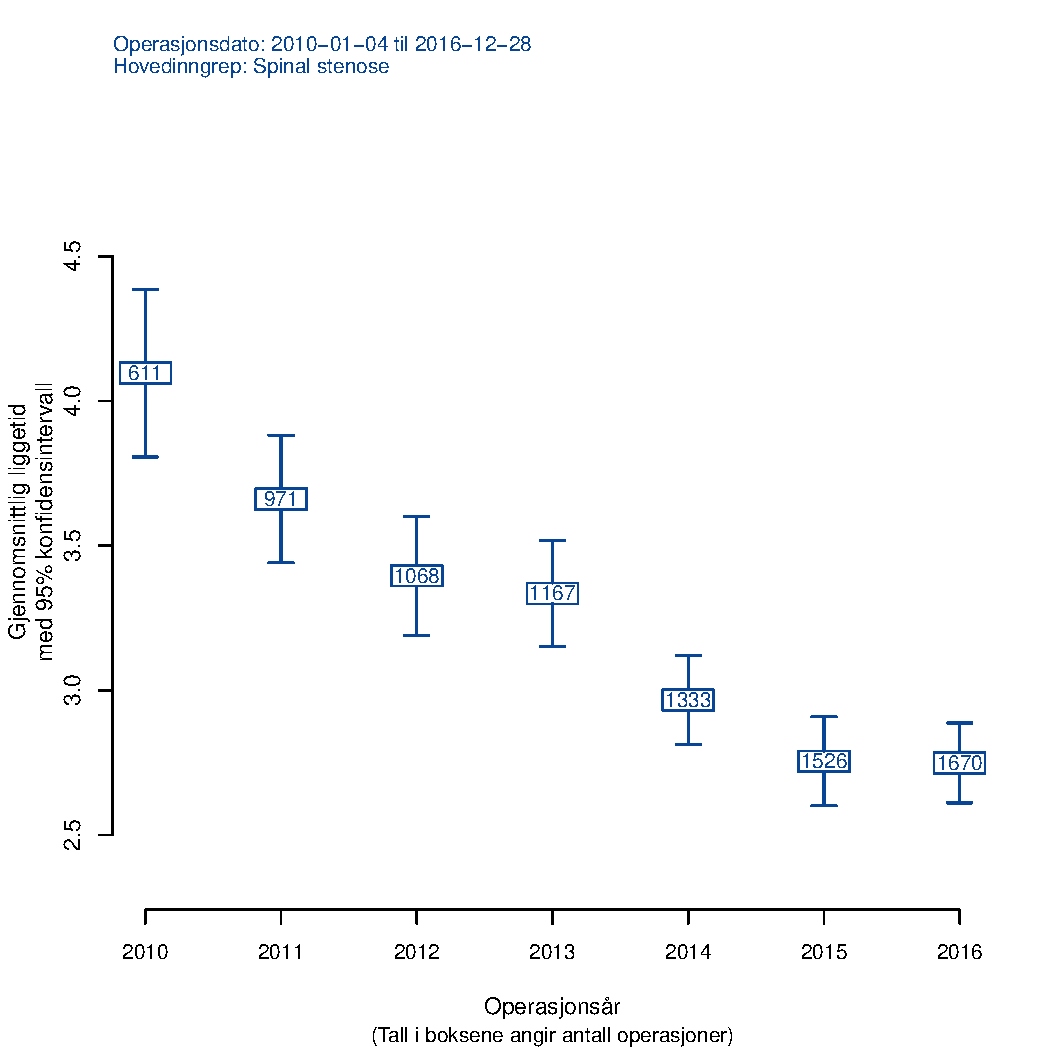
\includegraphics{Figurer/LiggetidBoxSS.pdf}}
}
\caption{Gjennomsnittlig liggetid for hhv. prolaps og spinal stenose. }
\label{fig:LiggedognTid}
\end{figure}

\begin{figure}[h] 
\scalebox{0.7}{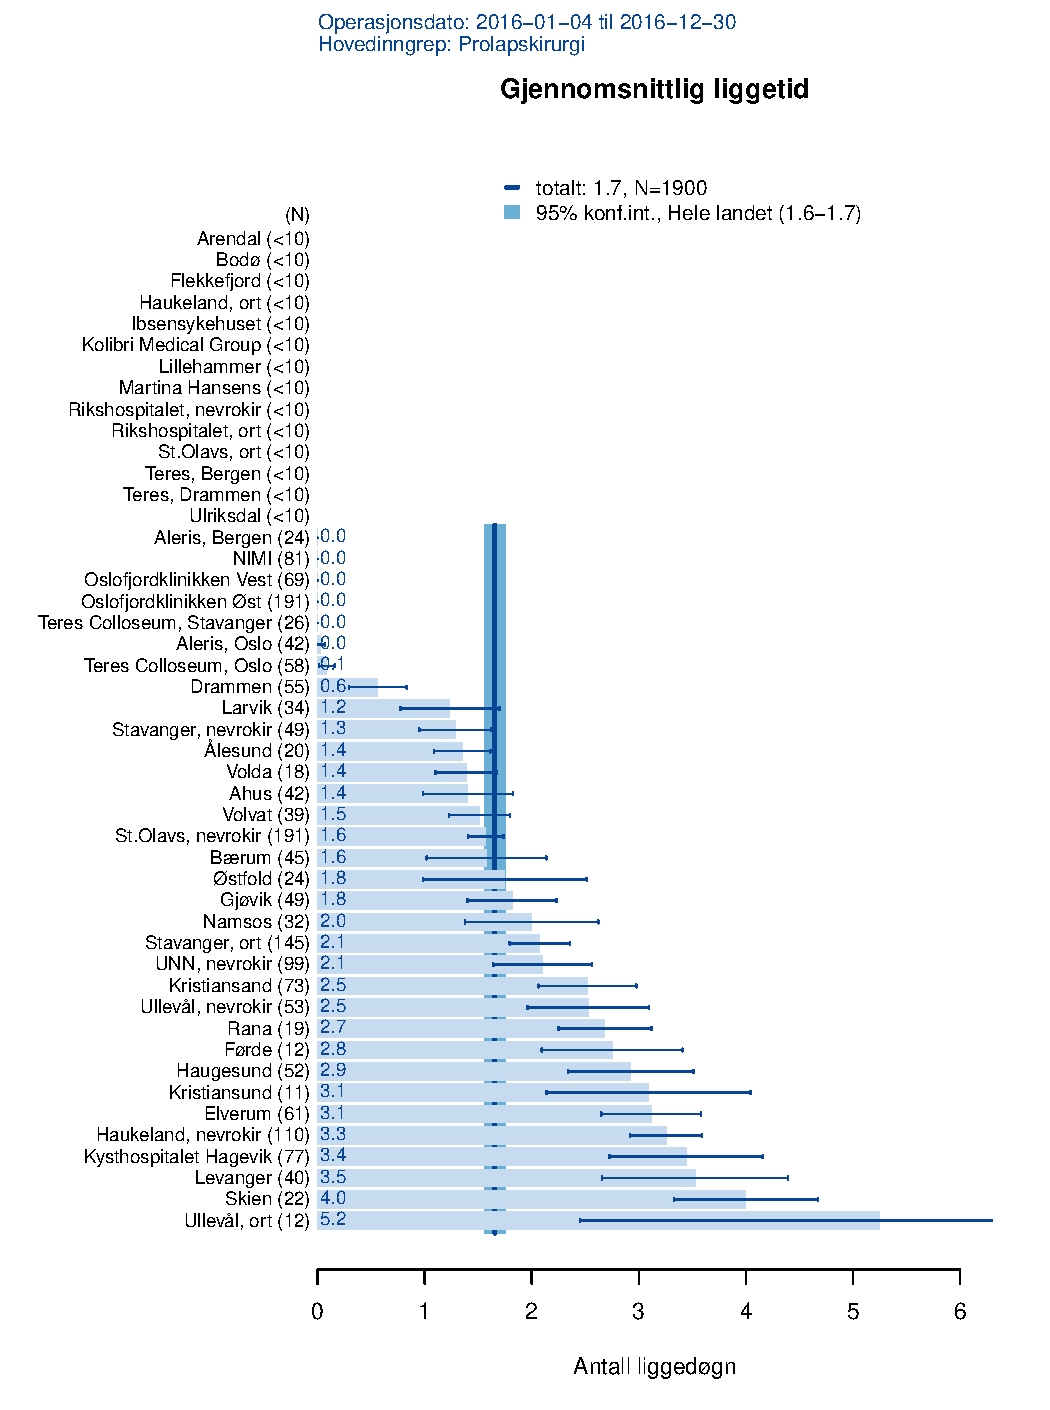
\includegraphics{Figurer/LiggetidAvdPro.pdf}}
\caption{Gjennomsnittlig liggetid for prolaps ved ulike avdelinger. Noen sykehus har kun dagkirurgi og får derfor få observasjoner. } 
\label{fig:LiggetidAvdPro}
\end{figure}

\begin{figure}[h] 
\scalebox{0.7}{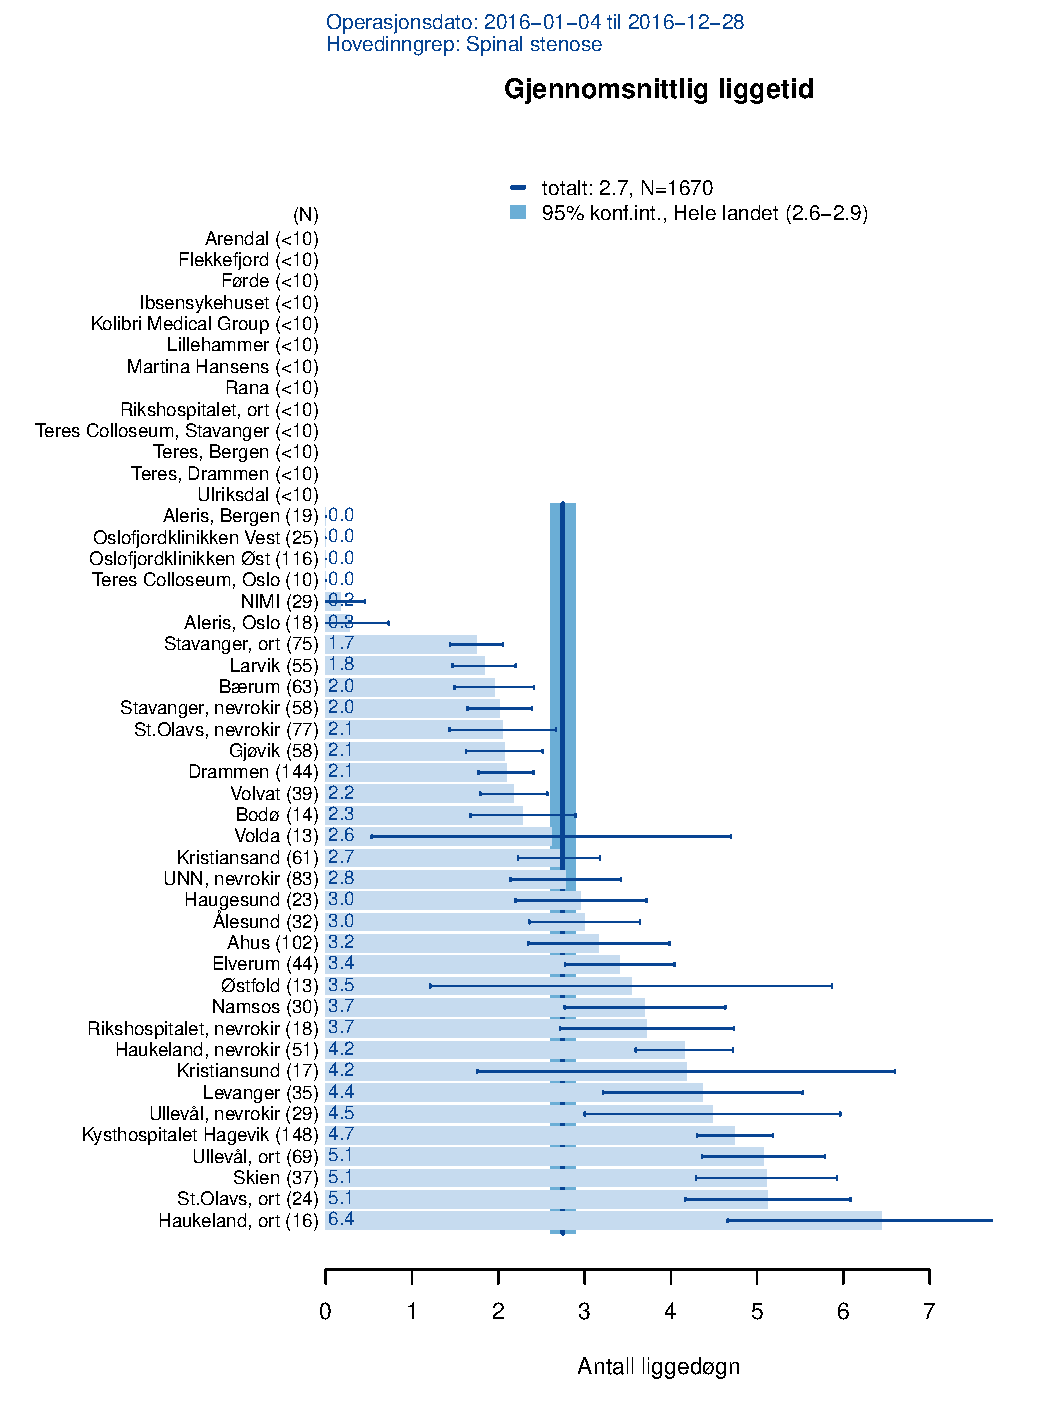
\includegraphics{Figurer/LiggetidAvdSS.pdf}}
\caption{Gjennomsnittlig liggetid for spinal stenose ved ulike avdelinger. Noen sykehus har kun dagkirurgi og får derfor få observasjoner. } 
\label{fig:LiggetidAvdSS}
\end{figure}






\clearpage

\section{Resultatmål}
All informasjon i dette kapitlet er hentet fra pasientskjema. Ingen av resultatmålene er justert
for eventuelle ulikheter i pasientpopulasjonene. Noen viktige forskjeller som kan forklare en del av forskjeller i resultat er vist i de forgående kapitlene.





\subsection{ Resultater etter ryggkirurgi, 2010 til 2016}



Hyppigst utførte inngrep er for prolaps, dernest for trang ryggkanal (spinal stenose),
dernest mer omfattende avstivningskirurgi (fusjon) for mer komplekse og
sammensatte tilstander. 
ODI er en score for smerterelatert fysisk funksjon og et sykdomsspesifikt livskvalitetsmål. Skalaen går fra 0
til 100, hvor 0 angir ingen funksjonshemming og følgelig beste livskvalitet.
Gjennomsnittlig ODI score var 46.7 før operasjon og 17.5 ett år etter
operasjon for prolapspasienter operert i 2015. Dette betyr at funksjonssvikten ble redusert fra alvorlig til minimal for gjennomsnittspasienten. \\

Pasienter operert for spinal stenose fikk også
betydelig bedring (ODI redusert fra 39.5 til 23.9), men mange har 
fortsatt moderat funksjonssvikt ett år etter kirurgi. 
De som ble operert med fusjon har
omtrent samme forbedring (ODI redusert fra 41.9 til 25.7). 
Dette betyr at selv om
pasientene kan forvente en betydelig bedring, vil mange fortsatt ha en del restplager
ett år etter kirurgi. Resultatene synes å være omtrent det samme fra år til år. NKR
sammenstiller nå norske resultater med data fra tilsvarende registre i Sverige og
Danmark. Foreløpige analyser tyder på at resultatene er de samme i
de tre nordiske landene.
Resultatene varierer imidlertid mye fra pasient til pasient og mellom sykehus.
Viktige årsaker til variasjon i operasjonsresultat er at ulike sykehus dels behandler
ulike pasientgrupper. Viktig for operasjonsresultatet er imidlertid fortsatt
indikasjonsstillingen («inngangsbilletten») til kirurgi; Fikk riktig person, rett
behandling til rett tid?

Forekomst av risikofaktorer blant pasientene påvirker operasjonsresultatene og kan
si noe om hvor godt behandlingstilbudet fungerer på ulike sykehus. Noen av disse
faktorene kan modifiseres/bedres gjennom bedre styring og planlegging av
virksomheten, strengere indikasjonsstilling og bedret pasientsikkerhet.





\subsection{Oswestry Disability Index (ODI)}

%Figur \ref{fig:OswEndr} viser gjennomsnittlig endring av ODI fra før operasjon til ett år etter.
Merk at resultatene \textit{ikke} er justert for forskjeller i pasientpopulasjonene. 




Figurene \ref{fig:OswEndrAvdPro} og \ref{fig:OswEndrAvdSS} viser gjennomsnittlig endring 12 måneder etter for hver avdeling for henholdsvis prolaps og spinal stenose pasienter. Forskjellene er små. Vi ser også at konfidensintervallene er relativt brede og overlappende.

\begin{figure}[h] 
\scalebox{0.7}{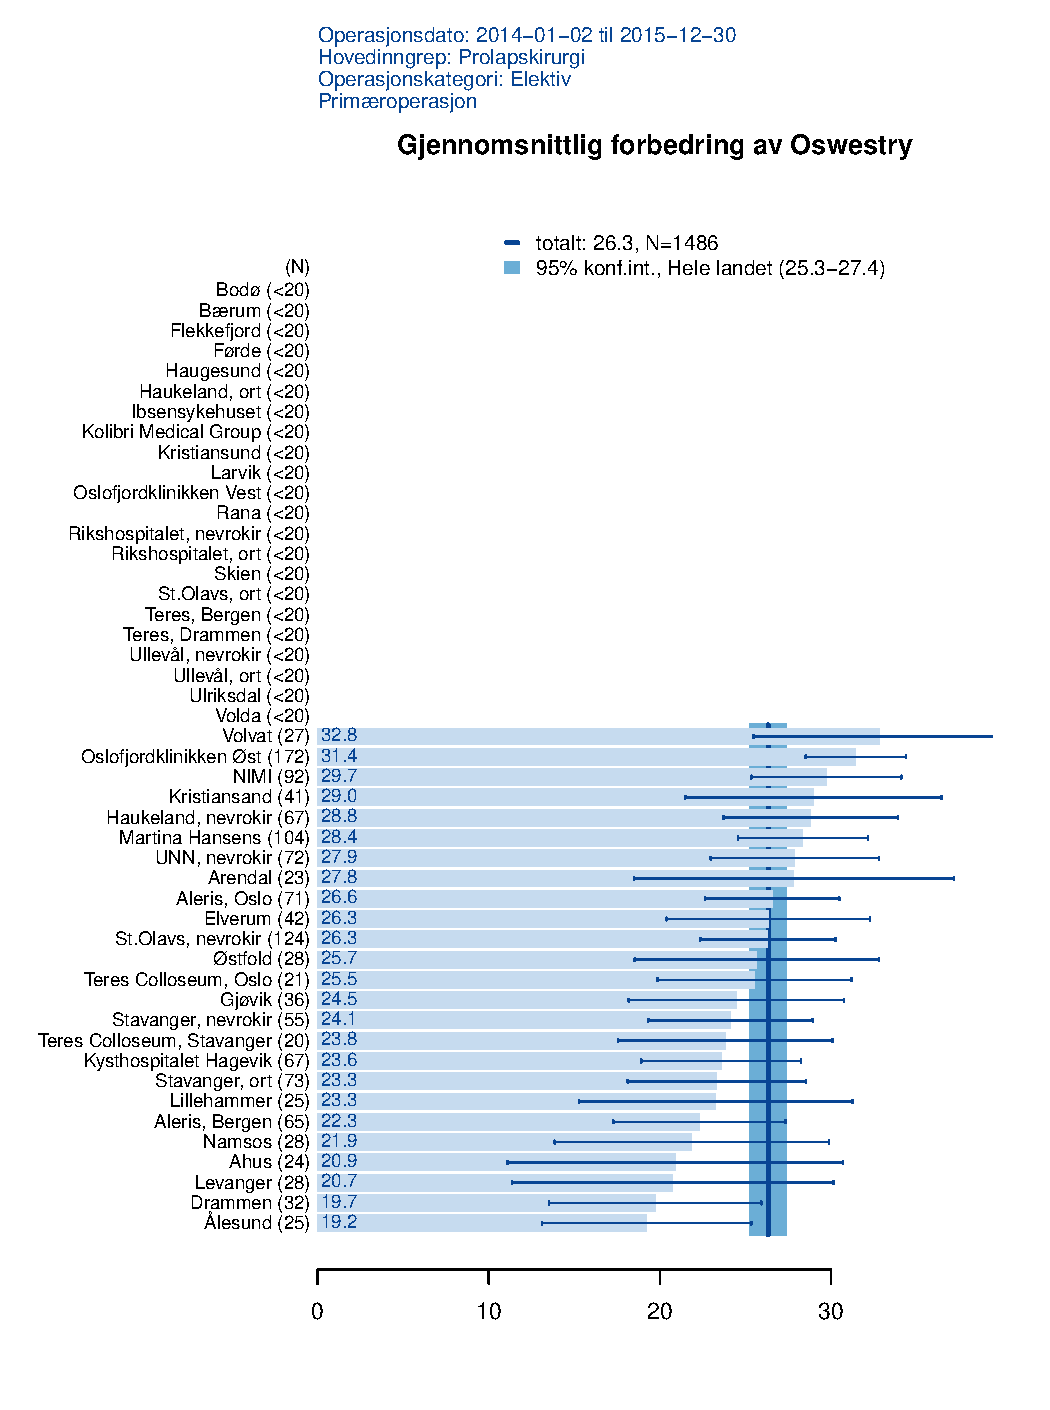
\includegraphics{Figurer/OswEndrAvdPro.pdf}}
\caption{Gjennomsnittlig endring av ODI per avdeling for prolaps}
\label{fig:OswEndrAvdPro}
\end{figure}

\begin{figure}[h] 
\scalebox{0.7}{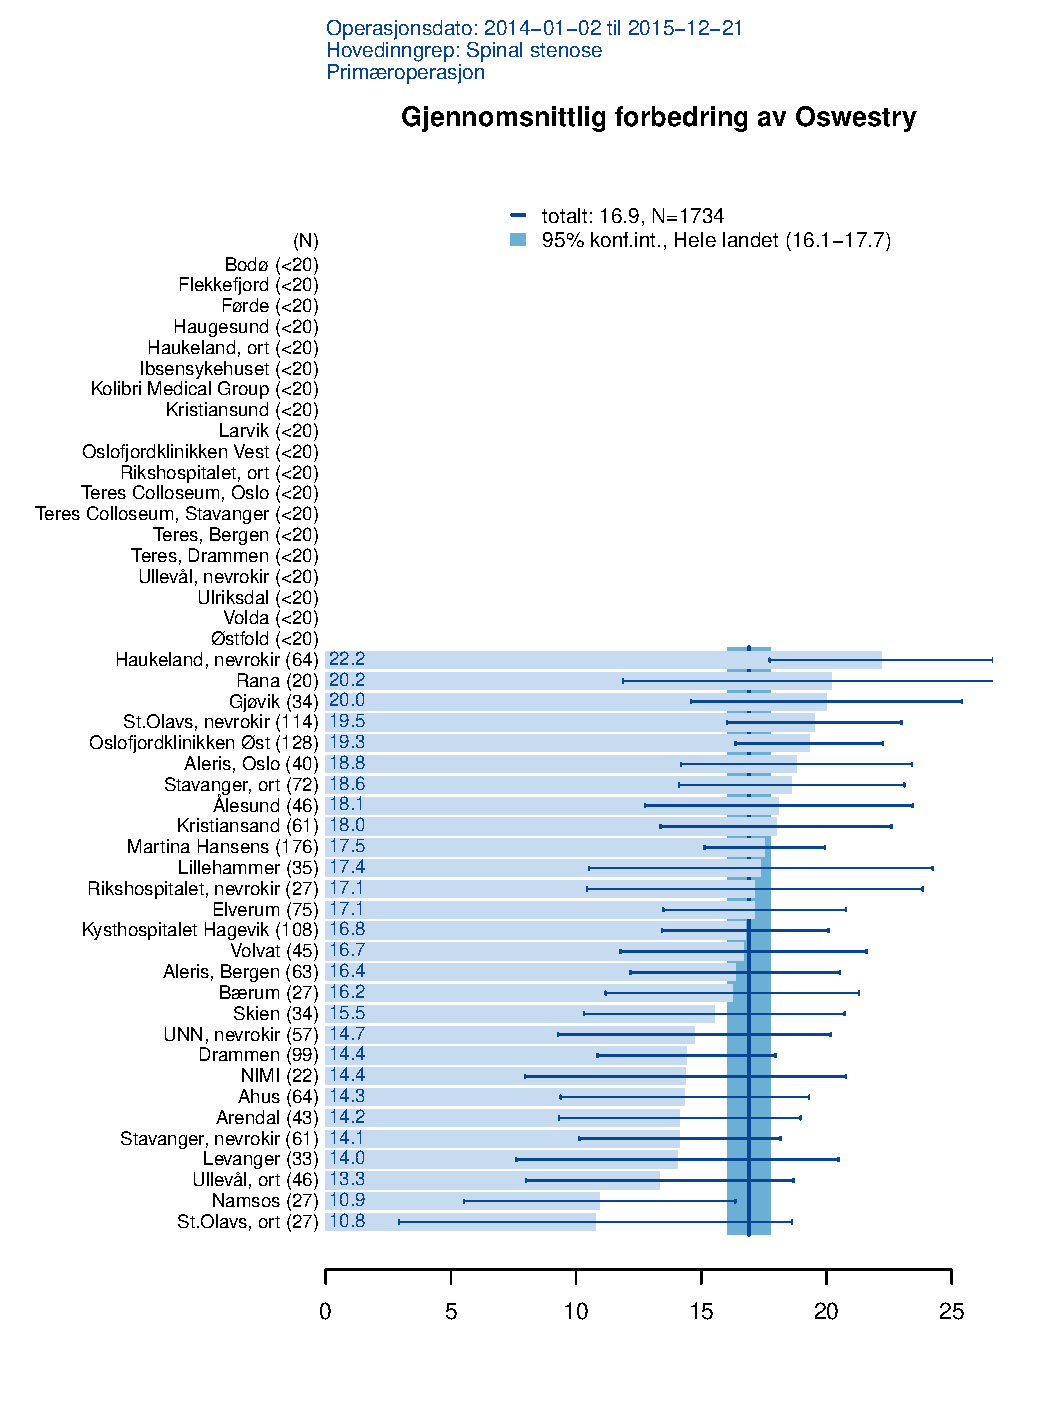
\includegraphics{Figurer/OswEndrAvdSS.pdf}}
\caption{Gjennomsnittlig endring av ODI per avdeling for spinal stenose.}
\label{fig:OswEndrAvdSS}
\end{figure}




Suksessrate, det vil si forbedring i Oswestry på mer enn 20 poeng, ligger stabilt rundt 60 \% for prolapspasienter, ett år etter operasjon. 
For spinal stenosepasienter er "suksess" forbedring i Oswestry på mer enn 30 \% , ett år etter operasjon. Denne raten ligger også stabilt rundt 60\%.


\clearpage


\subsection{Opplevd nytte av operasjon}

Figur \ref{fig:Nytte} viser hvor stor nytte pasientene opplever å ha hatt av behandlingen ett år etter operasjon fordelt på år. Tallet øverst på søyla angir antall pasienter som har svart. 
I figuren er det gjort følgende aggregering av svaralternativene i spørreskjemaet:
\begin{itemize}
\item ''Frisk mye/bedre'' omfatter ''helt bra'' og ''mye bedre'' 
\item ''Omtrent uendret'' omfatter ''litt bedre'', ''ingen endring'' og ''litt verre'' 
\item ''Klart verre'' omfatter ''mye verre'' og ''verre enn noen gang før''
\end{itemize}

Vi ser at en mindre andel av spinal stenose pasienter opplever å ha hatt stor nytte av operasjonen sammenlignet 
med prolapspasienter.



\begin{figure}[h] 
\begin{center}
\scalebox{0.55}{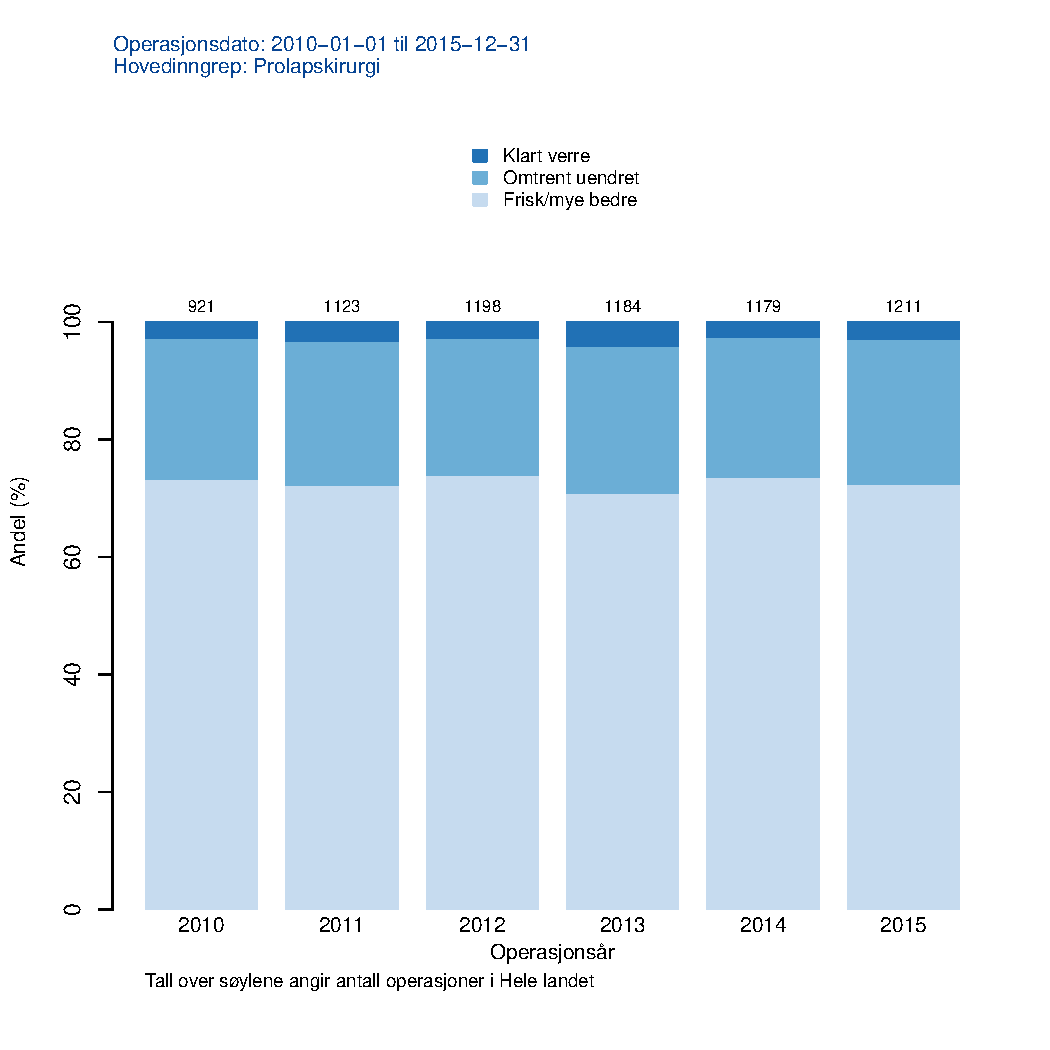
\includegraphics{Figurer/FigNyttePro.pdf}}
\scalebox{0.55}{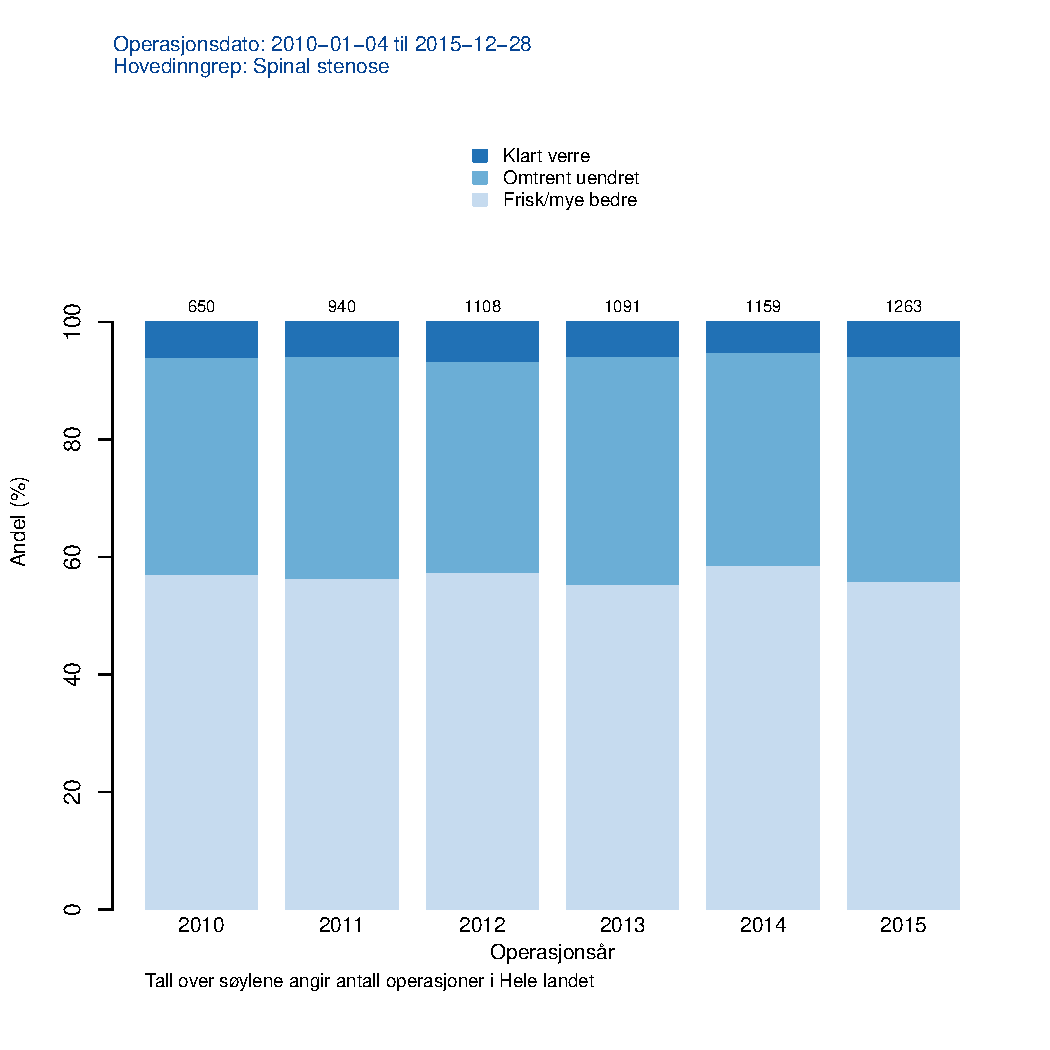
\includegraphics{Figurer/FigNytteSS.pdf}}
\end{center}
\caption{Spørsmål stilt 12 måneder etter operasjon til henholdsvis prolaps- og spinal stenosepasienter$:$ Hvilken nytte mener du at du har hatt av operasjonen?}
\label{fig:Nytte}
\end{figure}

\subsection{Pasienttilfredshet}

Figur \ref{fig:Fornoyd} viser hvor fornøyde pasientene var med behandlinga de fikk på sykehuset 12 mnd. 
etter operasjon fordelt på operasjonsår. Tallet øverst på søyla angir antall pasienter som har svart. Vi ser at spinal stenose pasienter gjennomgående er litt mindre fornøyde enn prolapspasienter.




\begin{figure}[h] 
\begin{center}
\scalebox{0.55}{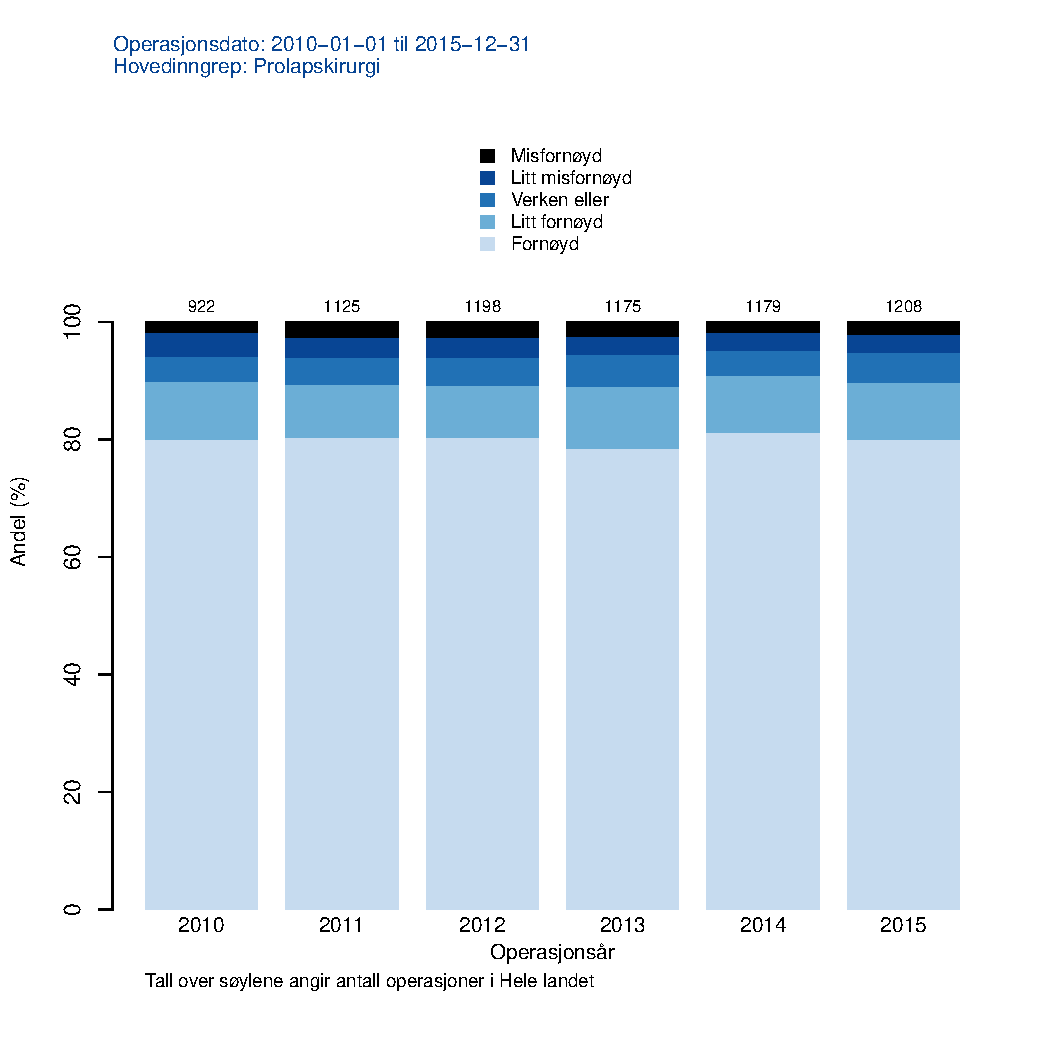
\includegraphics{Figurer/FigFornoydPro.pdf}}
\scalebox{0.55}{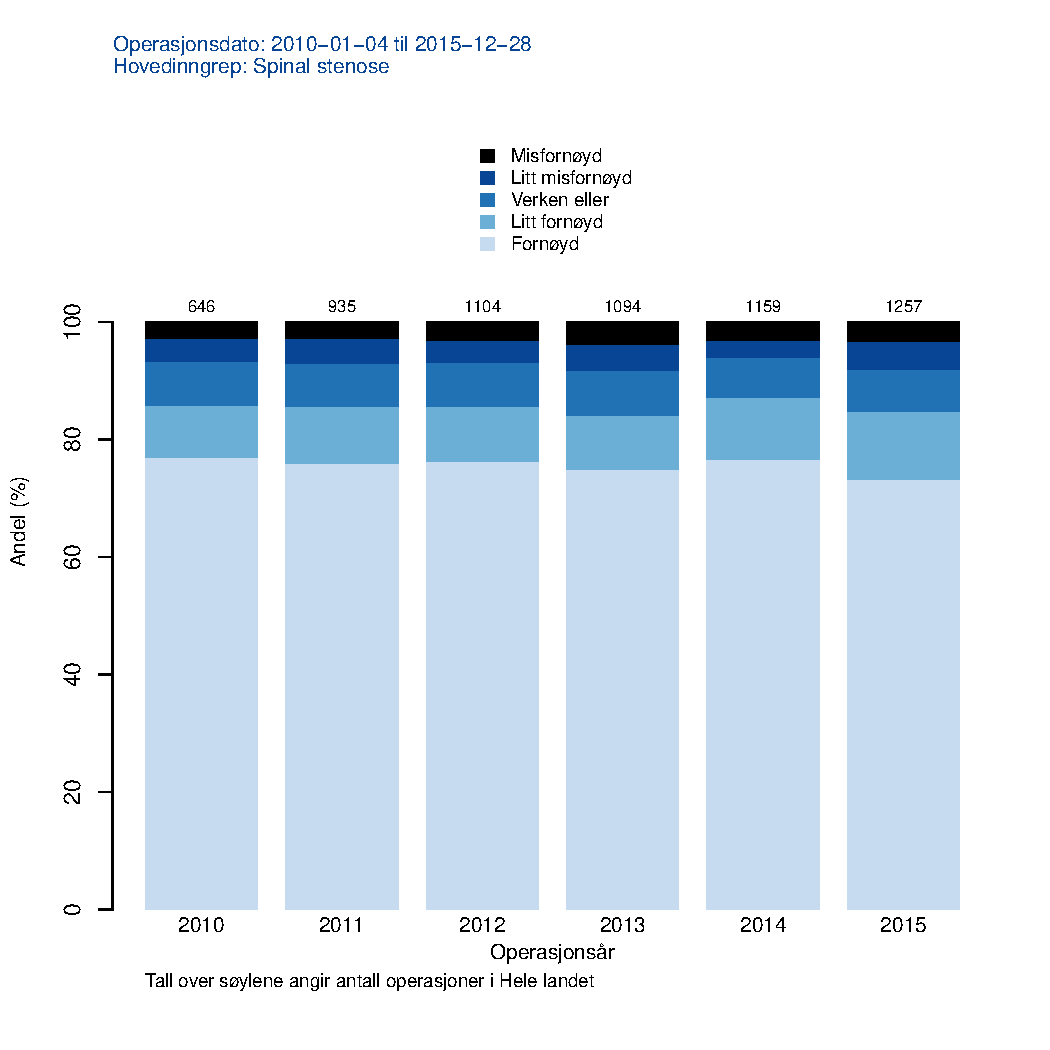
\includegraphics{Figurer/FigFornoydSS.pdf}}
\end{center}
\caption{Spørsmål stilt 12 måneder etter operasjon: Hvor fornøyd er du med behandlinga du har fått på sykehuset? til henholdsvis prolaps- og spinal stenosepasienter}
\label{fig:Fornoyd}
\end{figure}

\begin{figure}[h] 
\scalebox{0.7}{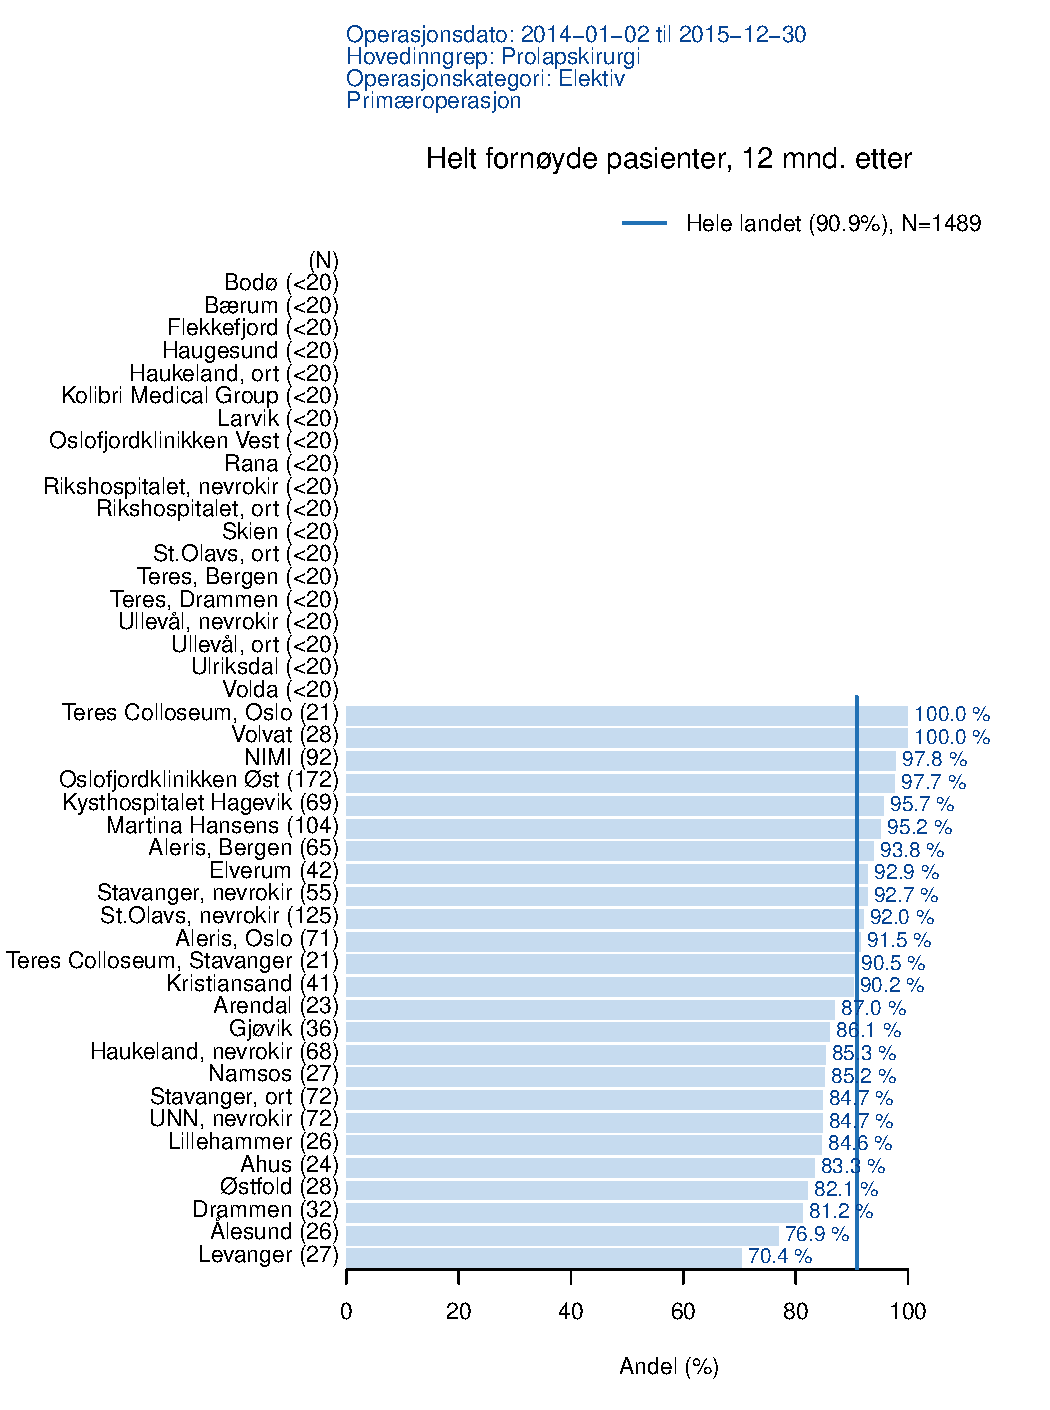
\includegraphics{Figurer/FigFornoydAvdPro.pdf}}
\caption{Prolapspasienter operert i 2014 og 2015, som ett år etter er helt fornøyde med behandlinga de har fått på sykehuset}
\label{fig:FornoydAvdPro}
\end{figure}

\begin{figure}[h] 
\scalebox{0.7}{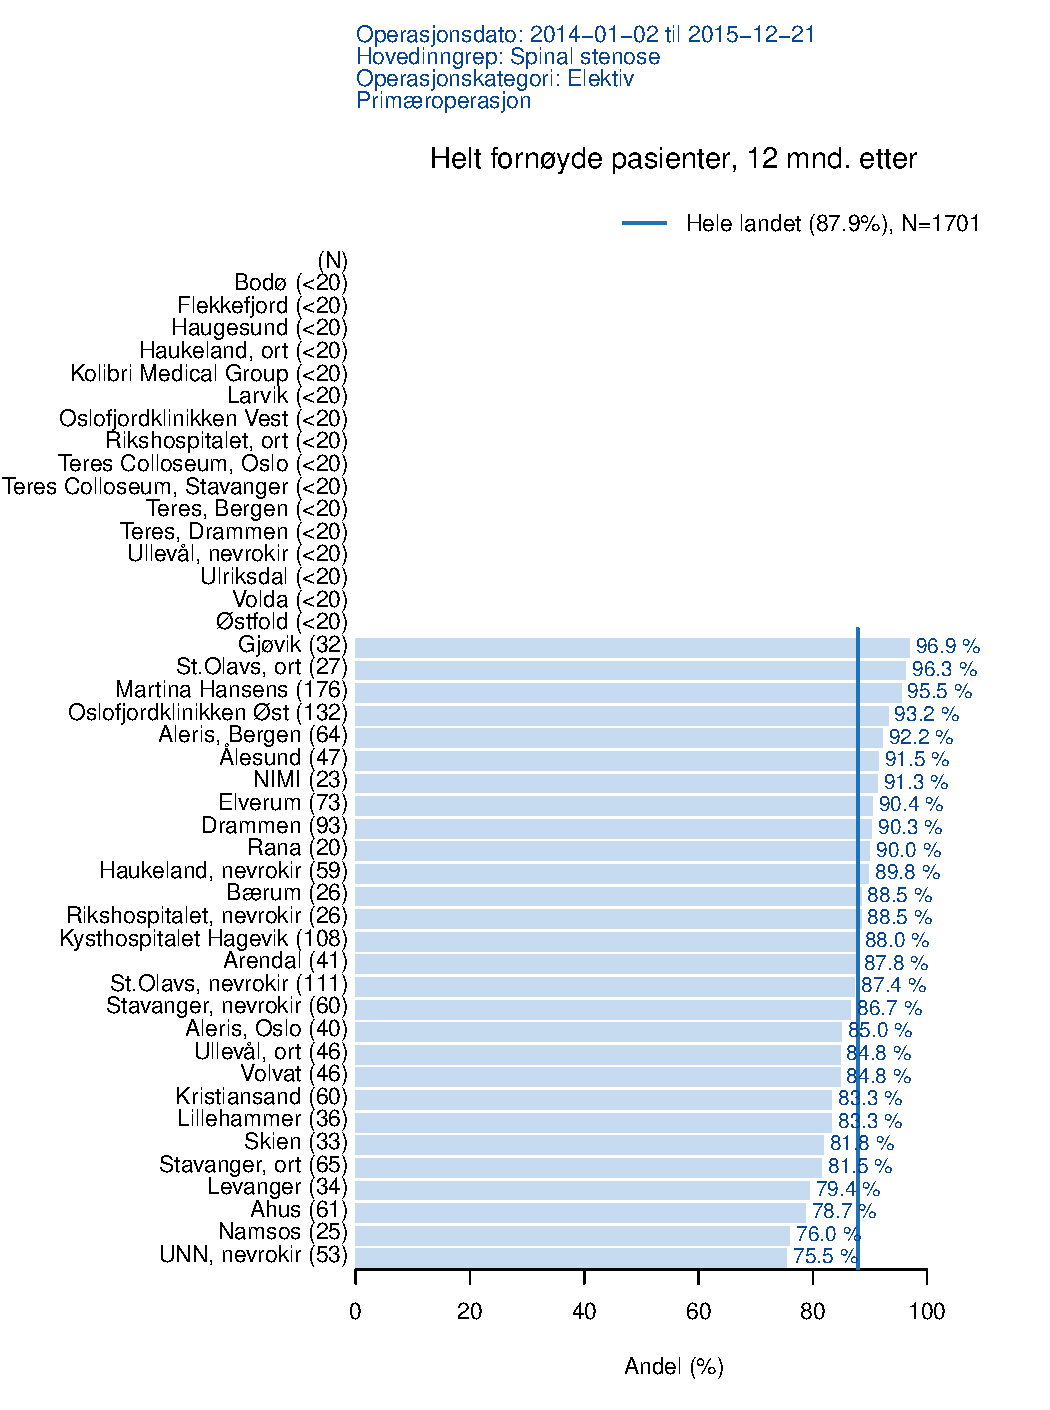
\includegraphics{Figurer/FigFornoydAvdSS.pdf}}
\caption{Spinal stenosespasienter som er helt fornøyde med behandlinga de har fått på sykehuset}
\label{fig:FornoydAvdSS}
\end{figure}


\subsection{Prolapskirurgi (alle kategorier)}



Gjennomsnittlig liggetid på sykehus i forbindelse med prolapsoperasjon har gått ned med 0.5 døgn fra 2010 til 2016.




Andelen som er operert ved hjelp av synsfremmende midler (mikroskop eller
lupebriller), som har åpenbare fordeler, har økt fra 81 \% i 2010 til 
99 \% i 2016 for prolapsoperasjoner. For spinal stenose er endringa fra 65 \% i 2010 til 
95 \% i 2016.





NKR har tidligere vist at multiple reoperasjoner har minimal effekt. Andelen som har vært operert mer enn 2 ganger tidligere ligger mellom 0.9 \%
og 1.5 \% for prolapspasienter og mellom 1.7 \%
og 3.1 \% for spinal stenosepasienter i perioden 2010-2016. 

Andelen prolapspasienter som ett år etter behandlinga er fornøyde med behandlingen de fikk på sykehuset (PREM) ligger mellom 79 \% og 81 \% for pasienter operert i perioden 2010-2015. 
Tilsvarende ligger andel fornøyde spinal stenosepasienter mellom 73 \% og 77 \%

\clearpage

\subsection{Kvalitetsindikatorer}

Kvalitetsindikatorene er  utviklet gjennom forskning (valideringsstudier)  i regi av NKR, Noen få er hentet fra annen internasjonal forskning.  Det er viktig å merke seg at "indikator" betyr en \textbf{mulig} sammenheng med kvalitet. Om det er mulig å gjøre endring på bakgrunn av indikatoren må vurderes ved de enkelte sykehus.

%\subsubsection{Sykehusvise resultater}



Resultatene nedenfor gjelder  \textit{planlagt, første gangs prolapsoperasjon}. 
Kun avdelinger med mer enn 10 evt. 20 (avhenger av type resultat) registrerte operasjoner i er med i
analysen. Grunnen til at gjentatt kirurgi (reoperasjon) og øyeblikkelig hjelp (ø-hjelp)
er filtrert bort er at dette er ulikt fordelt mellom sykehusene.


Følgende gjelder hele tidsperioden: Hos prolapspasienter operert som ø-hjelp er andelen med betydelig forbedring (suksessrate)  79.6 \%, mot 57.1 \% av de som blir operert planlagt (elektivt). Betydelig forbedring er definert som mer enn 20 poengs forbedring av ODI.
Hos prolapspasienter som ikke har vært operert i ryggen tidligere er suksessraten 63.4 \% mot 56.1 \%
hos de som har vært operert før. 
Langt færre pasienter i spinal stenosegruppen opereres som øyeblikkelig hjelp; 0.6 \%

Dersom man har vært operert mer enn 2 ganger tidligere i
ryggen, faller suksessraten for prolapsoperasjoner til 39.4 \%. 
For spinal stenose opererte faller suksessraten fra 48.3 \% til 40 \%. 
Sykehus som får henvist få pasienter som ø-hjelp og
mange til reoperasjon vil dermed få dårligere resultater.



\subsubsection{God indikasjonsstilling (rett pasient)}



Pasienter som har mye plager, vil kunne forvente størst nytte av ryggoperasjon,
mens de som har lite plager vil ha mindre potensial for forbedring og større risiko
for forverring. Gevinst av kirurgi henger derfor sammen med hvor streng
indikasjonsstillingen («inngangsbilletten» til kirurgi) har vært. Figur \ref{fig:BeinsmEndrPre} viser denne
sammenhengen tydelig. Det er verdt å merke seg er at hvis pasienten har lite smerter før
operasjon (bensmerter under 3 på den horisontale smerteskalaen), er det stor
sjanse for at pasienten faktisk blir verre (mindre enn 0 på den vertikale skalaen) etter
operasjon. \\
Figur \ref{fig:BeinsmLavPre} viser at det er stor variasjon i hvor stor grad sykehusene opererer
pasienter med prolaps og lite beinsmerter. Pasienter med lammelse (parese) er tatt
ut av analysen, da de ofte må opereres uansett grad av smerte.



\begin{figure}[ht]
\scalebox{0.7}{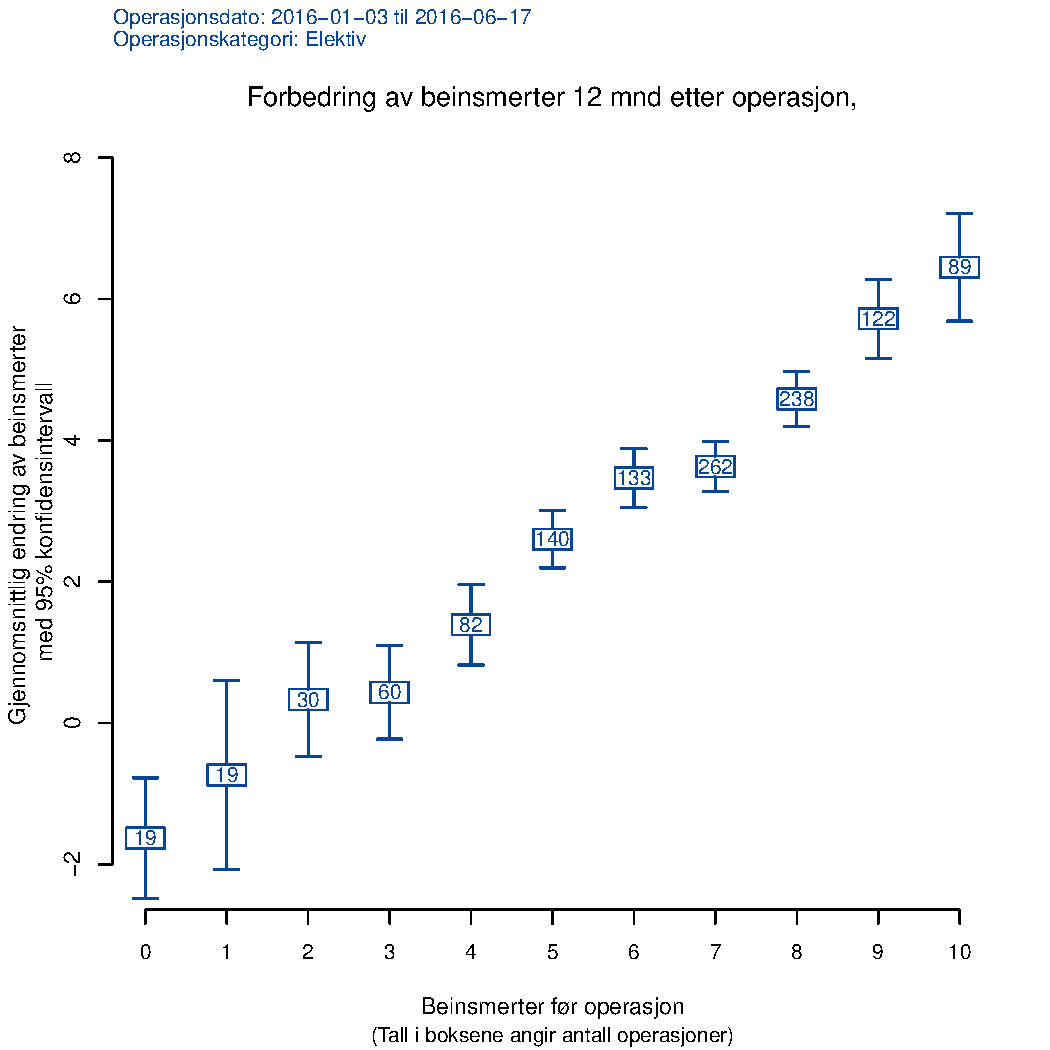
\includegraphics{Figurer/FigBeinsmEndrPre.pdf}}
\caption{\label{fig:BeinsmEndrPre}  Sammenheng mellom intensitet av bensmerte før operasjon og
forbedring etter operasjon. Skala for bensmerter går fra 0 til 10, hvor 0 betegner
ingen og 10 verst tenkelige smerte før operasjon (horisontal akse). Negativ endring
av bensmerten (vertikal akse) tilsvarer forverring, 0 betyr uendret smerte etter
operasjon.}
\end{figure}

\begin{figure}[ht]
\scalebox{0.7}{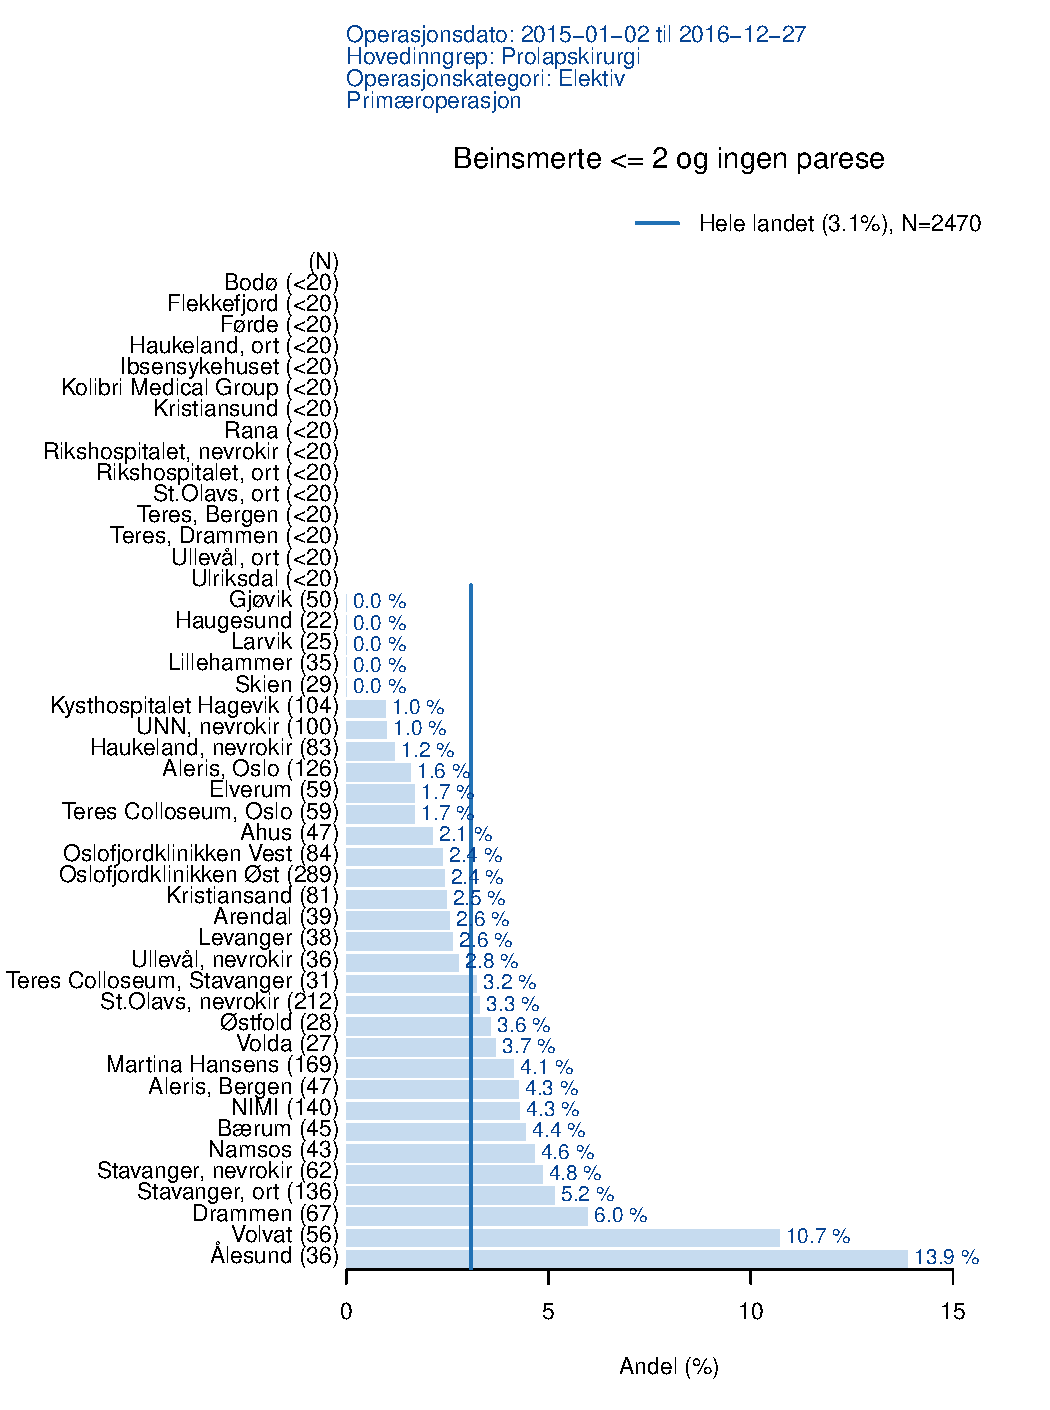
\includegraphics{Figurer/FigBeinsmLavPre.pdf}}
\caption{\label{fig:BeinsmLavPre}  Andel pasienter med lite beinsmerter ($\leq 2$) operert for prolaps.}
\end{figure}






\subsubsection{Resultatindikatorer (behandlings-effektivitet)}

Viktige tiltak for å bedre behandlingseffektivitet vil være å øke andelen som får en
betydelig forbedring (suksessraten), redusere andelen som ikke har nytte av
behandlingen, blir verre eller får komplikasjoner. Nedenfor vises noen indikatorer
(«bench-mark kriterier») som NKR har utviklet og validert for
behandlingseffektivitet sammen med forekomst av de hyppigste komplikasjonene.
Forskjellene skyldes dels at pasientgruppene som opereres ved ulike sykehus har
ulik risikoprofil. Resultatene som vist i figurene nedenfor er ikke justert for disse
forskjellene. Kunnskap om risiko kan dette bidra til bedre utvelgelse av pasienter til
kirurgi.





\subsubsection{Uønsket resultat}

Pasienter som 1 år etter prolapskirurgi har en ODIskår over 48 har fortsatt alvorlig
smerterelatert funksjonshemming i dagliglivet. Figur \ref{fig:Osw48} viser andelen som har ODIskår over 48 etter prolapsoperasjon. Flesteparten av disse pasientene vil
oppfatte sin livssituasjon som klart verre enn før operasjonen. 

\begin{figure}[ht]
\scalebox{0.7}{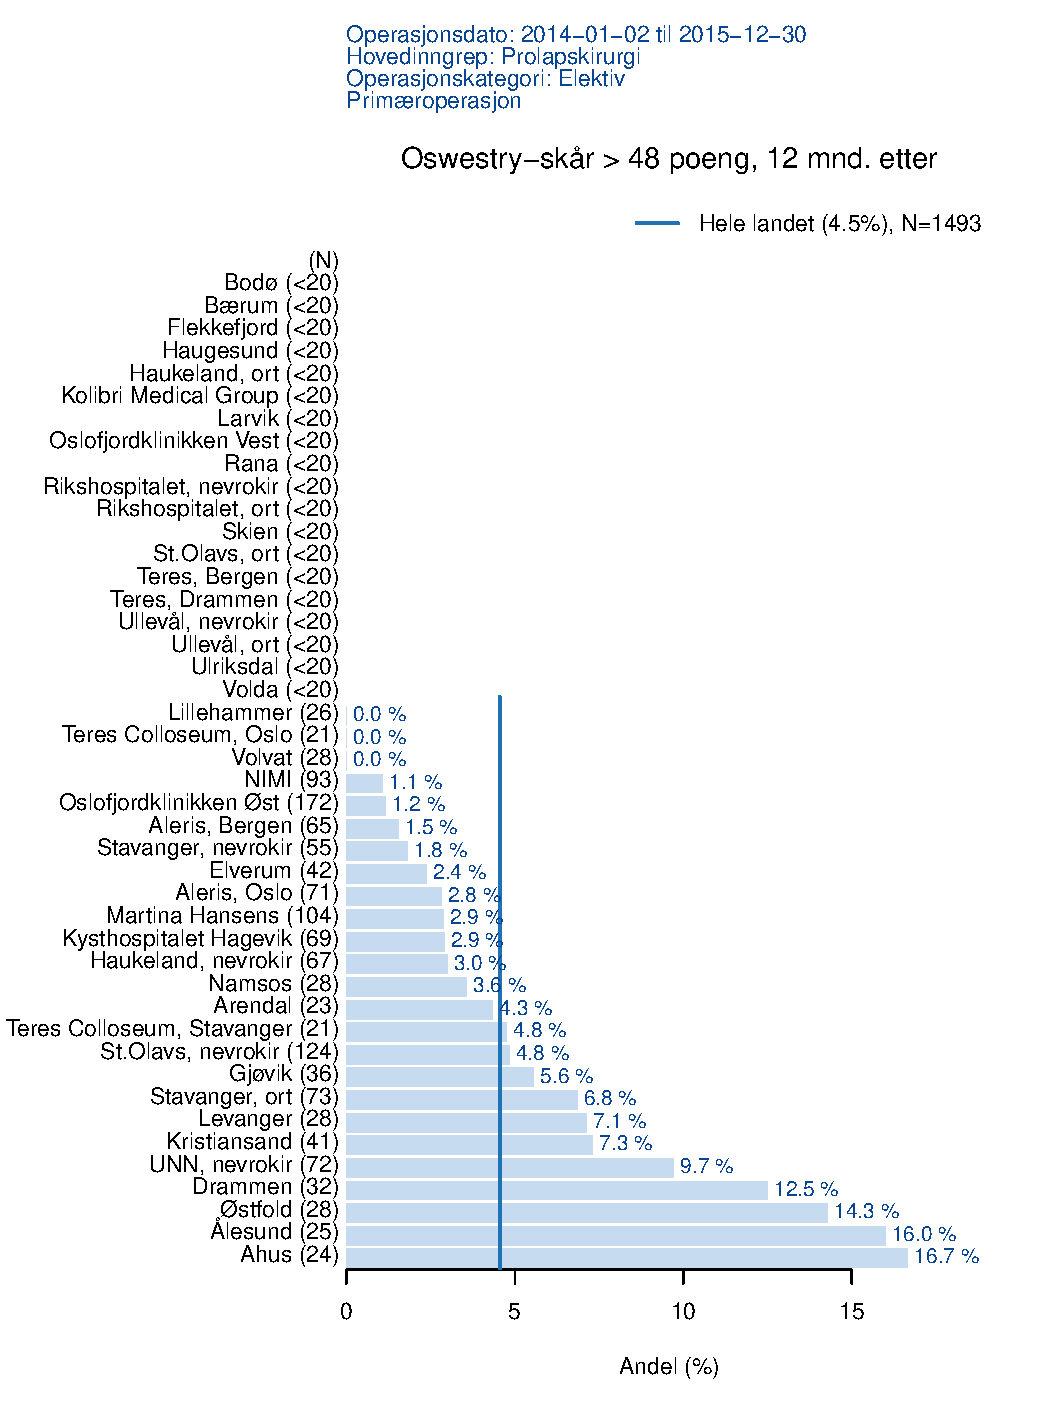
\includegraphics{Figurer/FigOsw48.pdf}}
\caption{\label{fig:Osw48}  Andel pasienter med alvorlig smerterelatert funksjonssvikt 1 år etter
prolapskirurgi. Pasienter operert i 2014 og 2015.}
\end{figure}



Pasienter med forbedring av ODI skår mindre enn 13 vil som hovedregel ikke
oppfatte sin situasjon som vesentlig forbedret etter kirurgi. Resultatet blir dermed å
betrakte som utilfredsstillende. Figur \ref{fig:OswEndrLav} viser andelen med lav forbedring av ODIskår ved hver avdeling.

\begin{figure}[ht]
\scalebox{0.7}{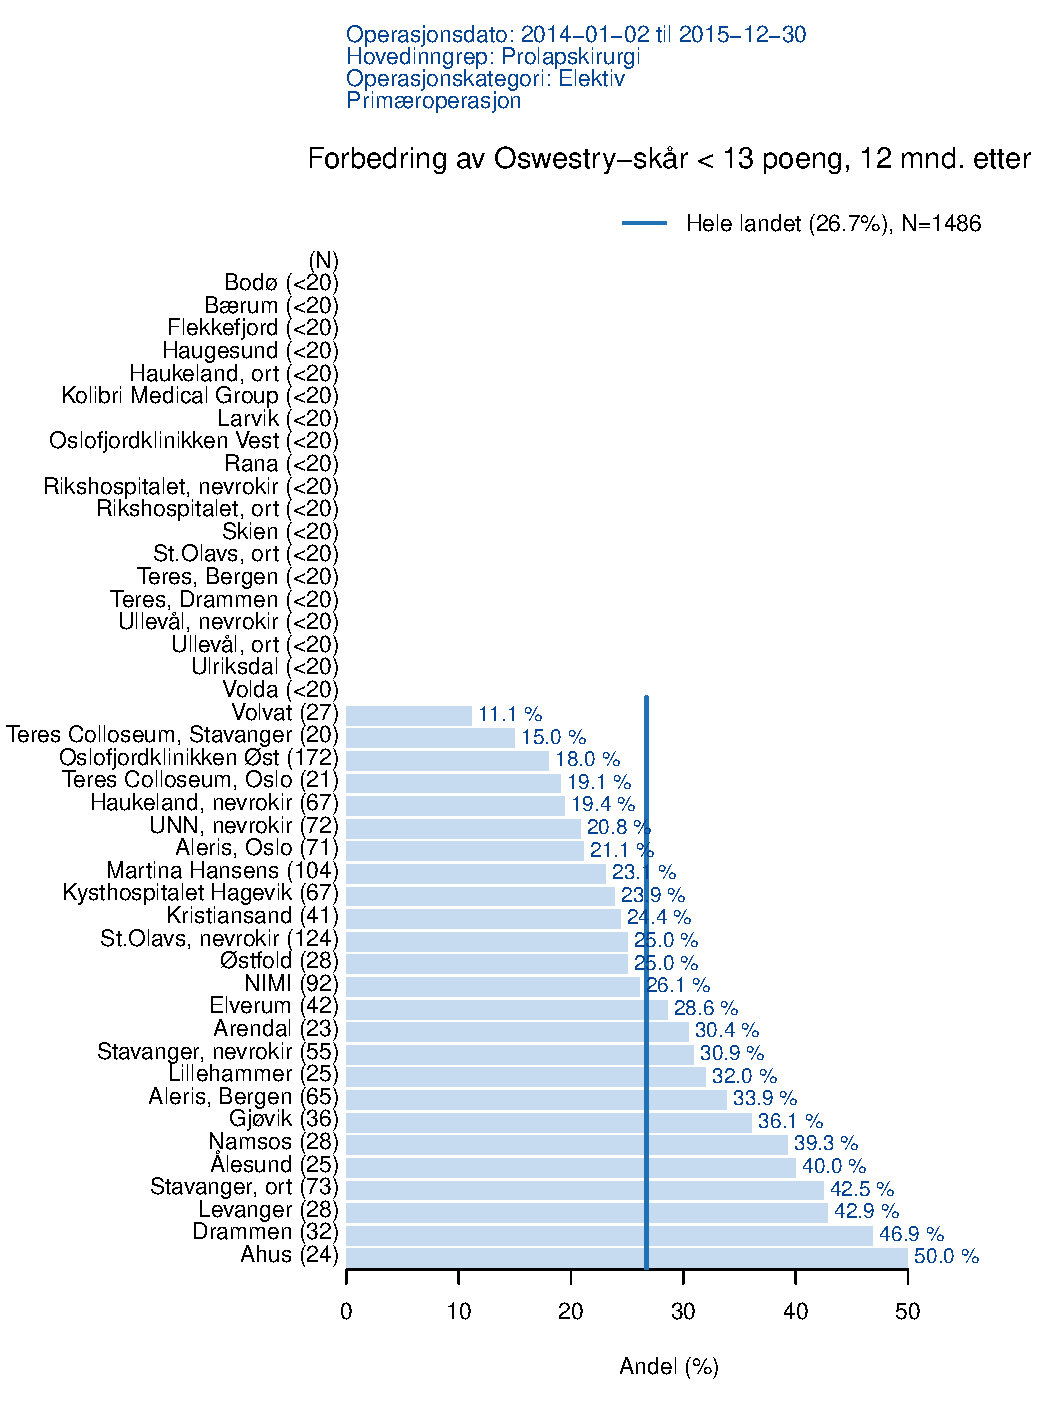
\includegraphics{Figurer/FigOswEndrLav.pdf}}
\caption{\label{fig:OswEndrLav}   Andel pasienter som ikke oppnår et tilfredsstillende resultat, ODI
forbedring under 13 poeng, etter prolapskirurgi. Pasienter operert i 2014 og 2015.}
\end{figure}




















\subsubsection{Ønsket resultat («suksess»)}
ODI skår  under 22 poeng oppleves av de fleste pasientene som et helt akseptabelt fysisk funksjonsnivå 12 mnd etter ryggopersjon. Figurene \ref{fig:Osw22Pro} og \ref{fig:Osw22SS} angir hvor stor andel av henholdsvis prolaps og spinal stenose opererete som oppnår dette.

\begin{figure}[ht]
\scalebox{0.7}{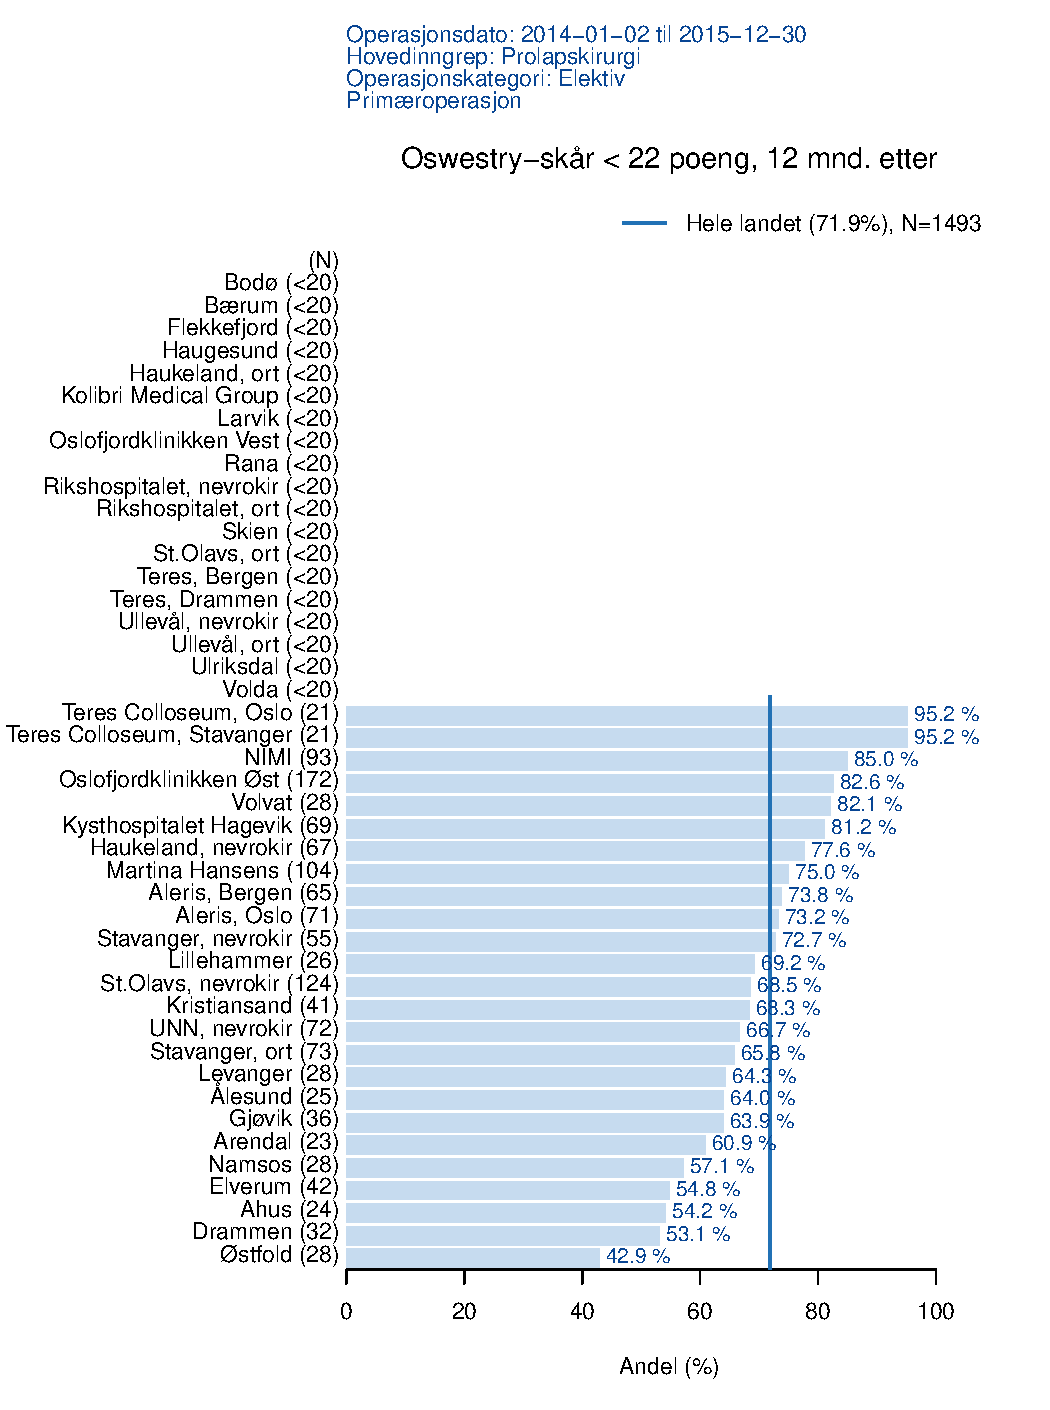
\includegraphics{Figurer/FigOsw22Pro.pdf}}
\caption{\label{fig:Osw22Pro}   Andel pasienter med ODI under 22 ett år
etter prolapsoperasjon. Pasienter operert i 2014 og 2015.}
\end{figure}

\begin{figure}[ht]
\scalebox{0.7}{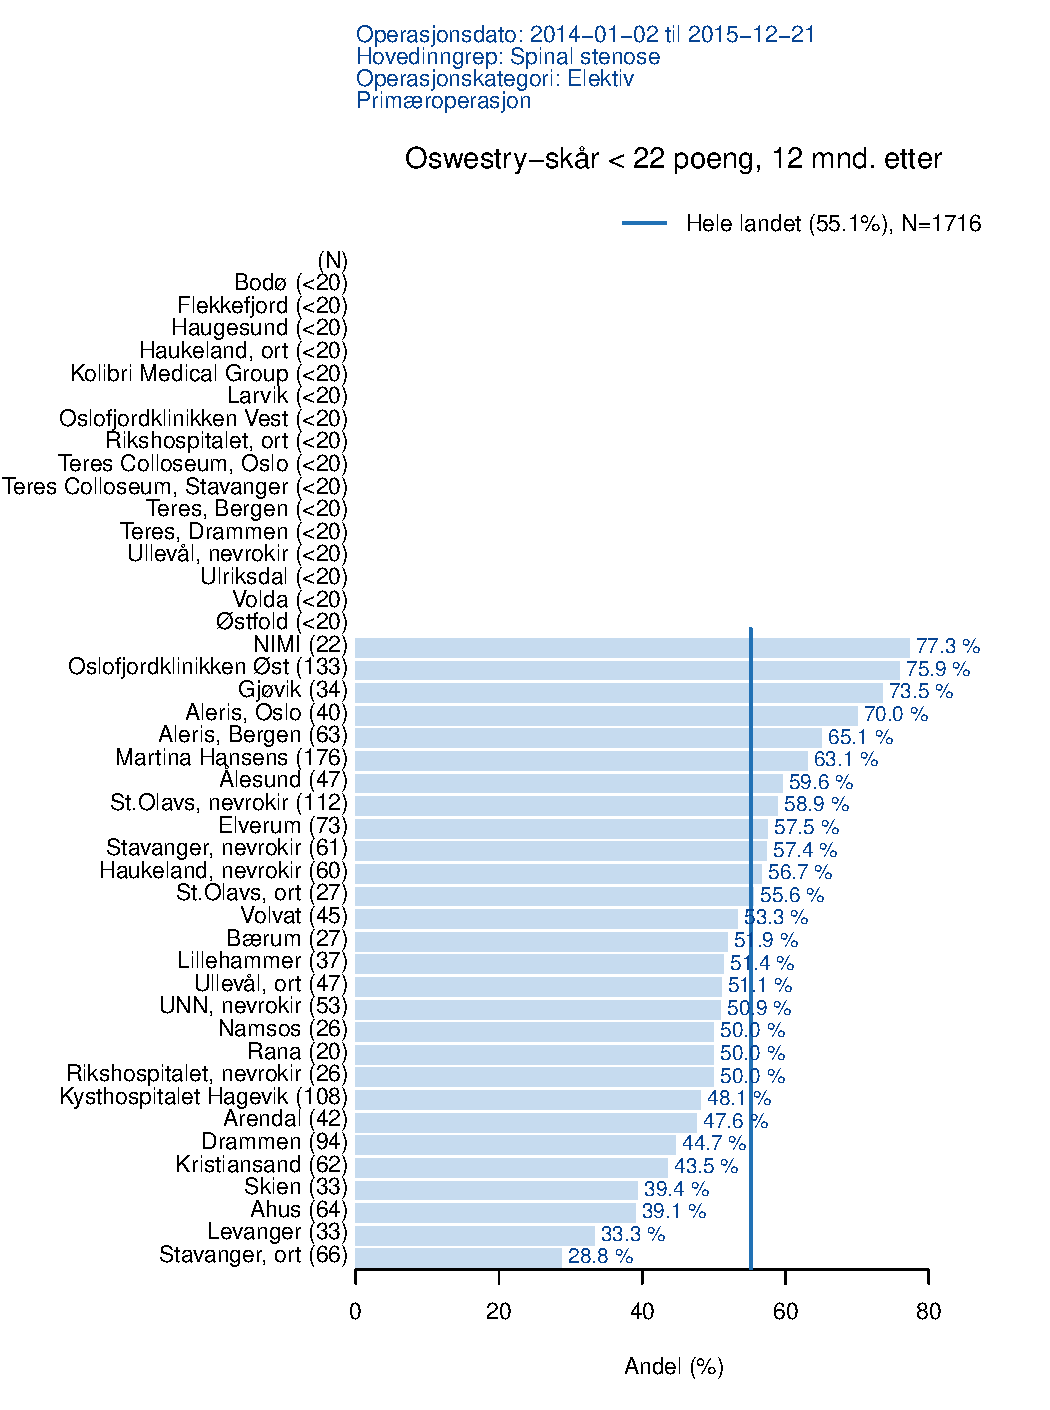
\includegraphics{Figurer/FigOsw22SS.pdf}}
\caption{\label{fig:Osw22SS}   Andel pasienter med ODI under 22 ett år
etter spinal stenose operasjon. Pasienter operert i 2014 og 2015.}
\end{figure}



Figur \ref{fig:OswEndr20} viser andel pasienter med betydelig forbedring av selvrapportert
smerterelatert funksjon i dagliglivet («suksess», ODI forbedring over 20 poeng) 1 år
etter prolapsoperasjon.

\begin{figure}[ht]
\scalebox{0.7}{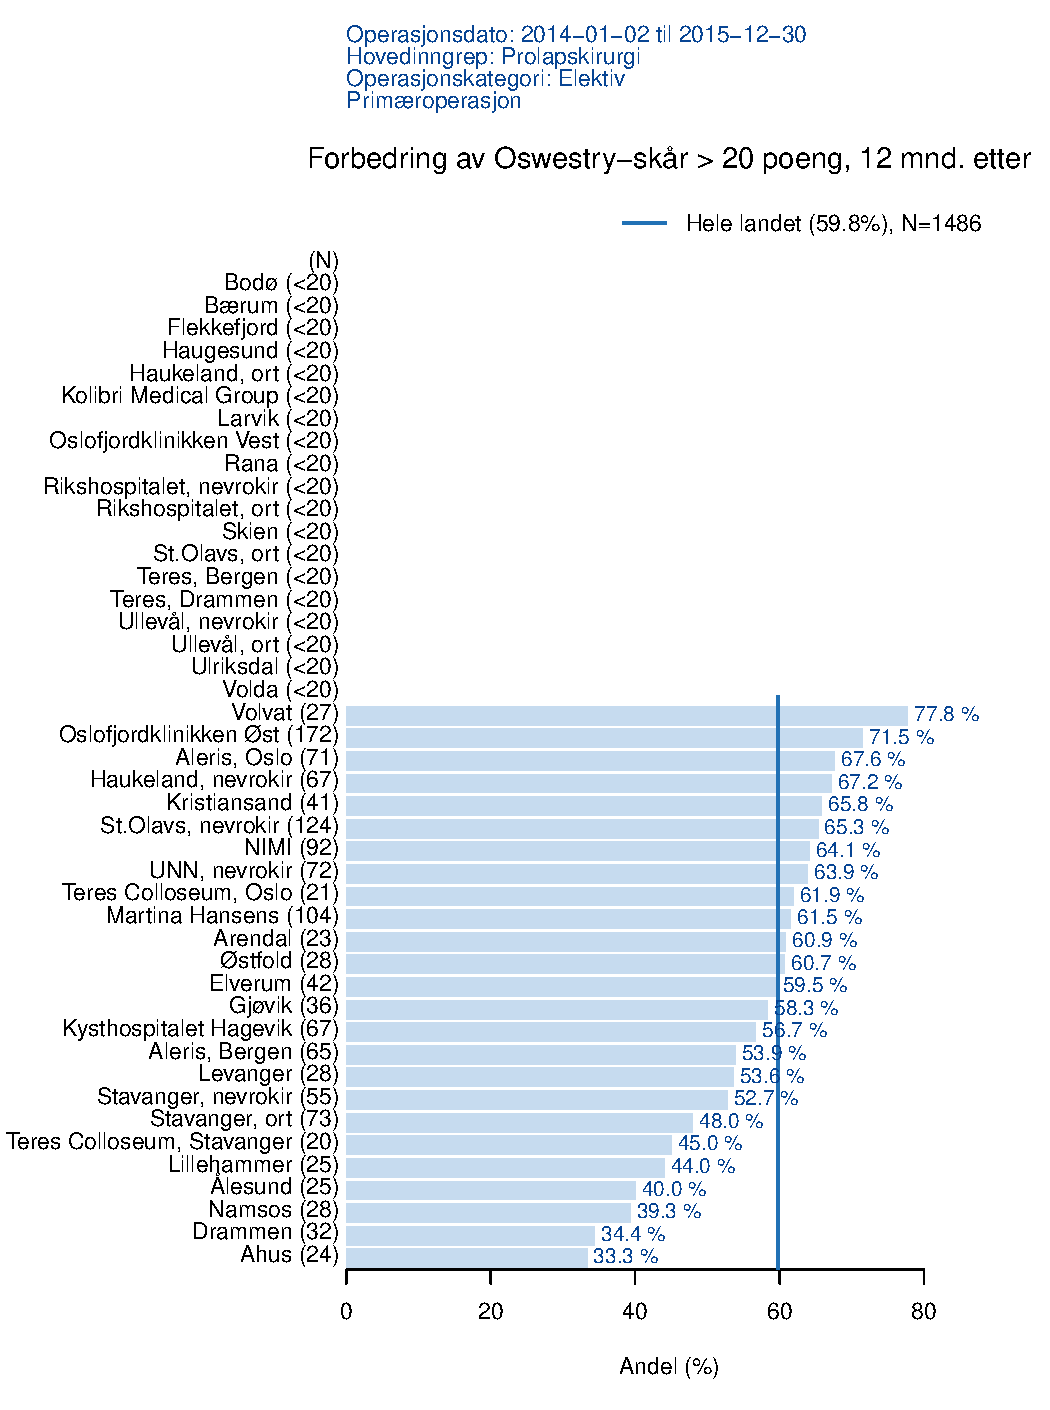
\includegraphics{Figurer/FigOswEndr20.pdf}}
\caption{\label{fig:OswEndr20}   Andel pasienter med betydelig forbedring av selvrapportert
smerterelatert funksjon i dagliglivet («suksess», ODI forbedring over 20 poeng) 1 år
etter prolapsoperasjon. Pasienter operert i 2014 og 2015.}
\end{figure}



Nyere forskning knyttet til NKR viser at pasienter operert for spinal stenose bør ha minst 30 \% forbedring av ODI for å oppleve et meget godt operasjonsresultat. Figur \ref{fig:OswEndr30pstSS} viser andelen med minst 30 \% forbedring av ODI ved hver avdeling.

\begin{figure}[ht]
\scalebox{0.7}{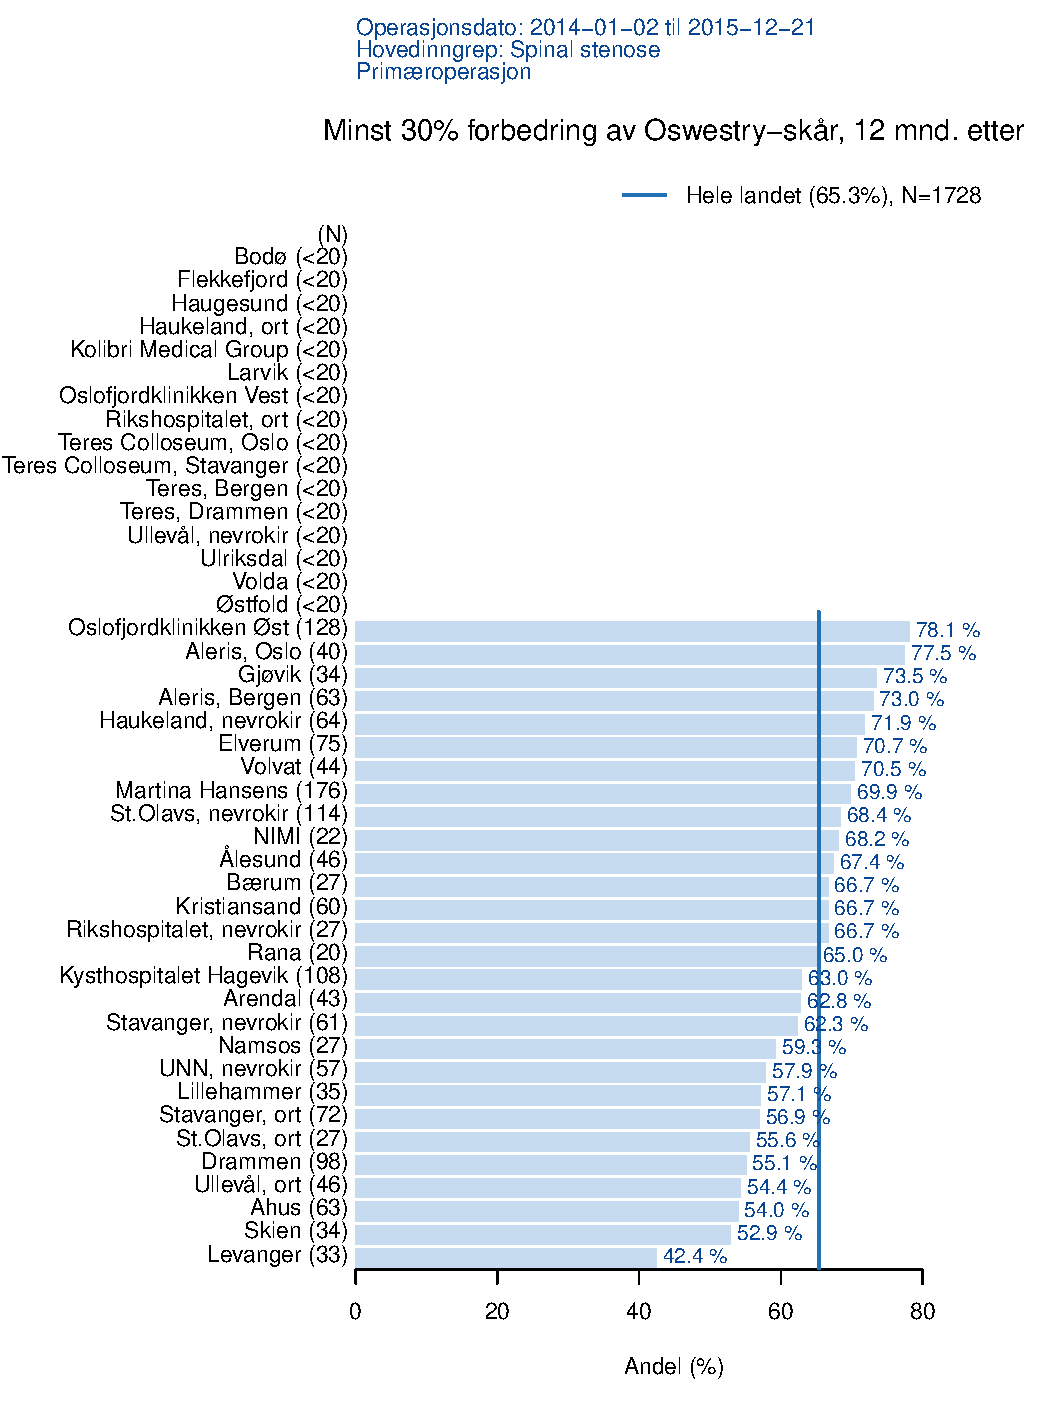
\includegraphics{Figurer/FigOswEndr30pstSS.pdf}}
\caption{\label{fig:OswEndr30pstSS} Andel spinal stenose pasienter med betydelig forbedring av selvrapportert
smerterelatert funksjon i dagliglivet («suksess», ODI forbedring over 30 \% poeng) 1 år
etter prolapsoperasjon. Pasienter operert i 2014 og 2015.}
\end{figure}













\subsubsection{Komplikasjoner (sikkerhet)}

\textbf{I. Sårinfeksjon.}

For alle typer prolapsoperasjoner har
andel sårinfeksjoner (pasientrapportert) har blitt noe redusert fram til 2010, mens bruk av  forbyggende antibiotikabehandling har økte sterkt og i dag får nesten alle forebyggende antibiotikabehandling ved kirurgi. Siden 2010 har andelen sårinfeksjoner ligget stabilt rundt 2 \% for prolapsopererte og rundt 3 \% for spinal stenose opererte.


%\begin{figure}[ht]
%      \centering \scalebox{s2}{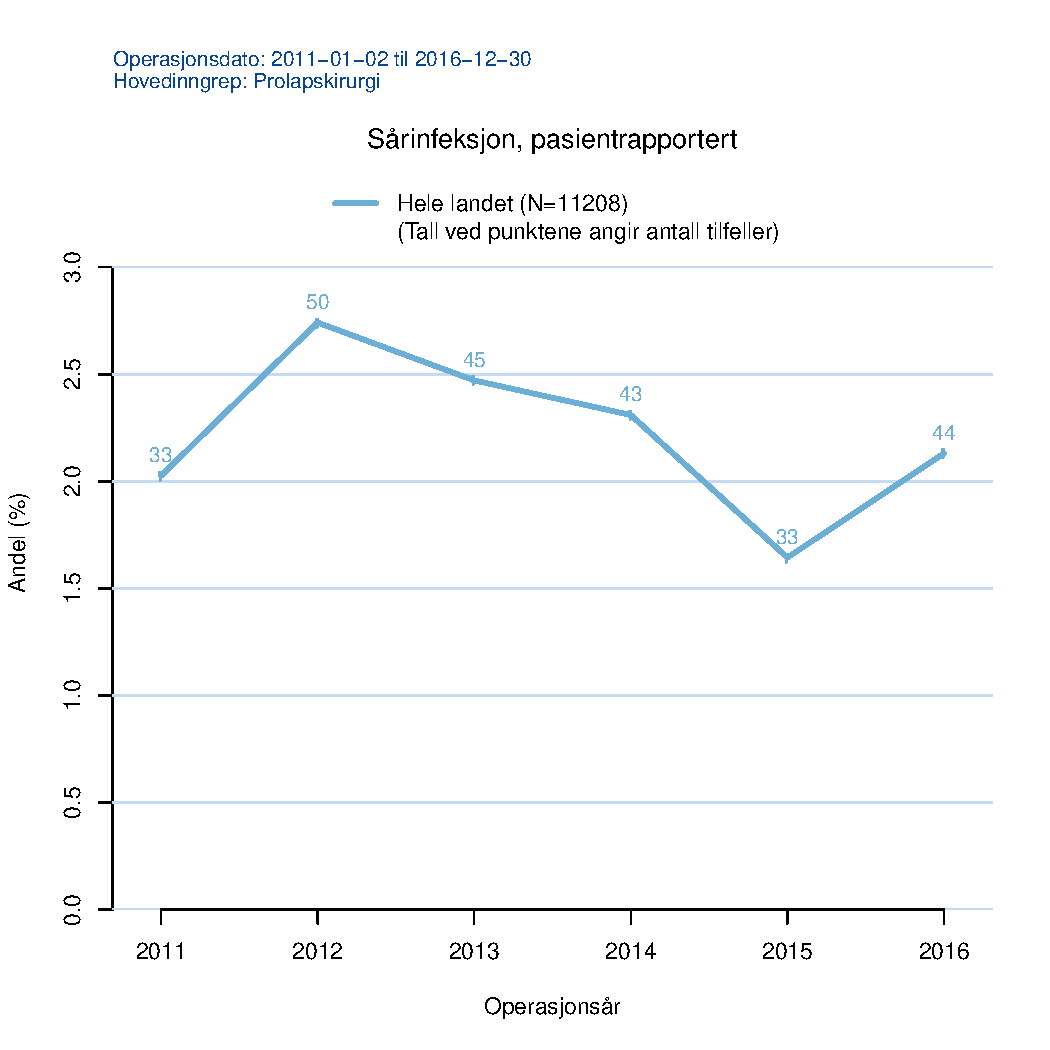
\includegraphics{Figurer/FigKpInf3MndTidPro.pdf}}
%      \centering \scalebox{s2}{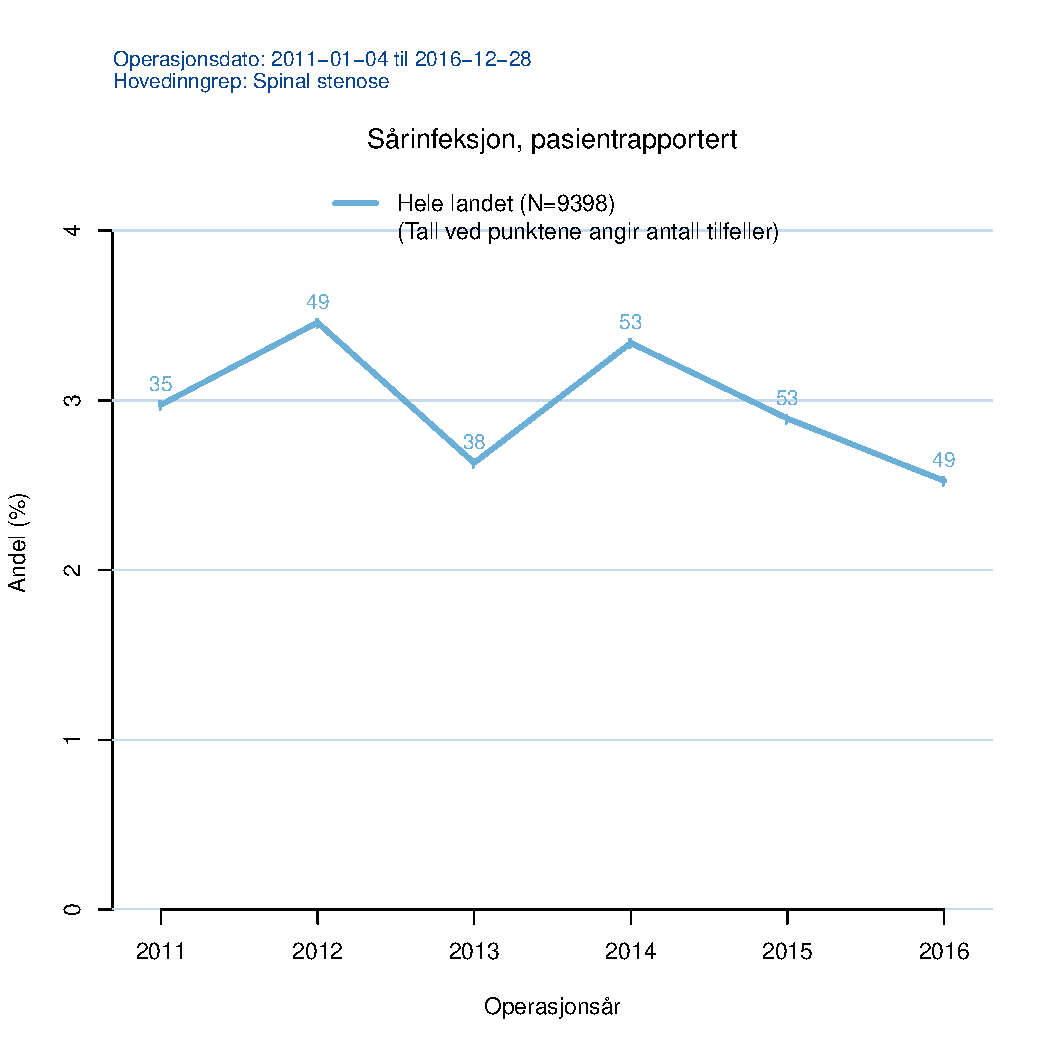
\includegraphics{Figurer/FigKpInf3MndTidSS.pdf}}
%      \caption{\label{fig:KpInfTid} Andel pasienter som rapporterer om sårinfeksjon 3 måneder etter
%hhv. prolapskirurgi og spinal stenose, utvikling over tid.}
%\end{figure}

Årsakene til sårinfeksjon er komplekse. I 2016 fikk 98-100 \% av pasienter som
opereres for prolaps, forebyggende antibiotikabehandling under operasjon. NKR
viste for mange år siden at dette har god forbyggende effekt. Figurene \ref{fig:KpInfAvdPro} og \ref{fig:KpInfAvdSS} viser andel pasienter som får sårinfeksjon ved hver avdeling.

\begin{figure}[ht]
\scalebox{0.7}{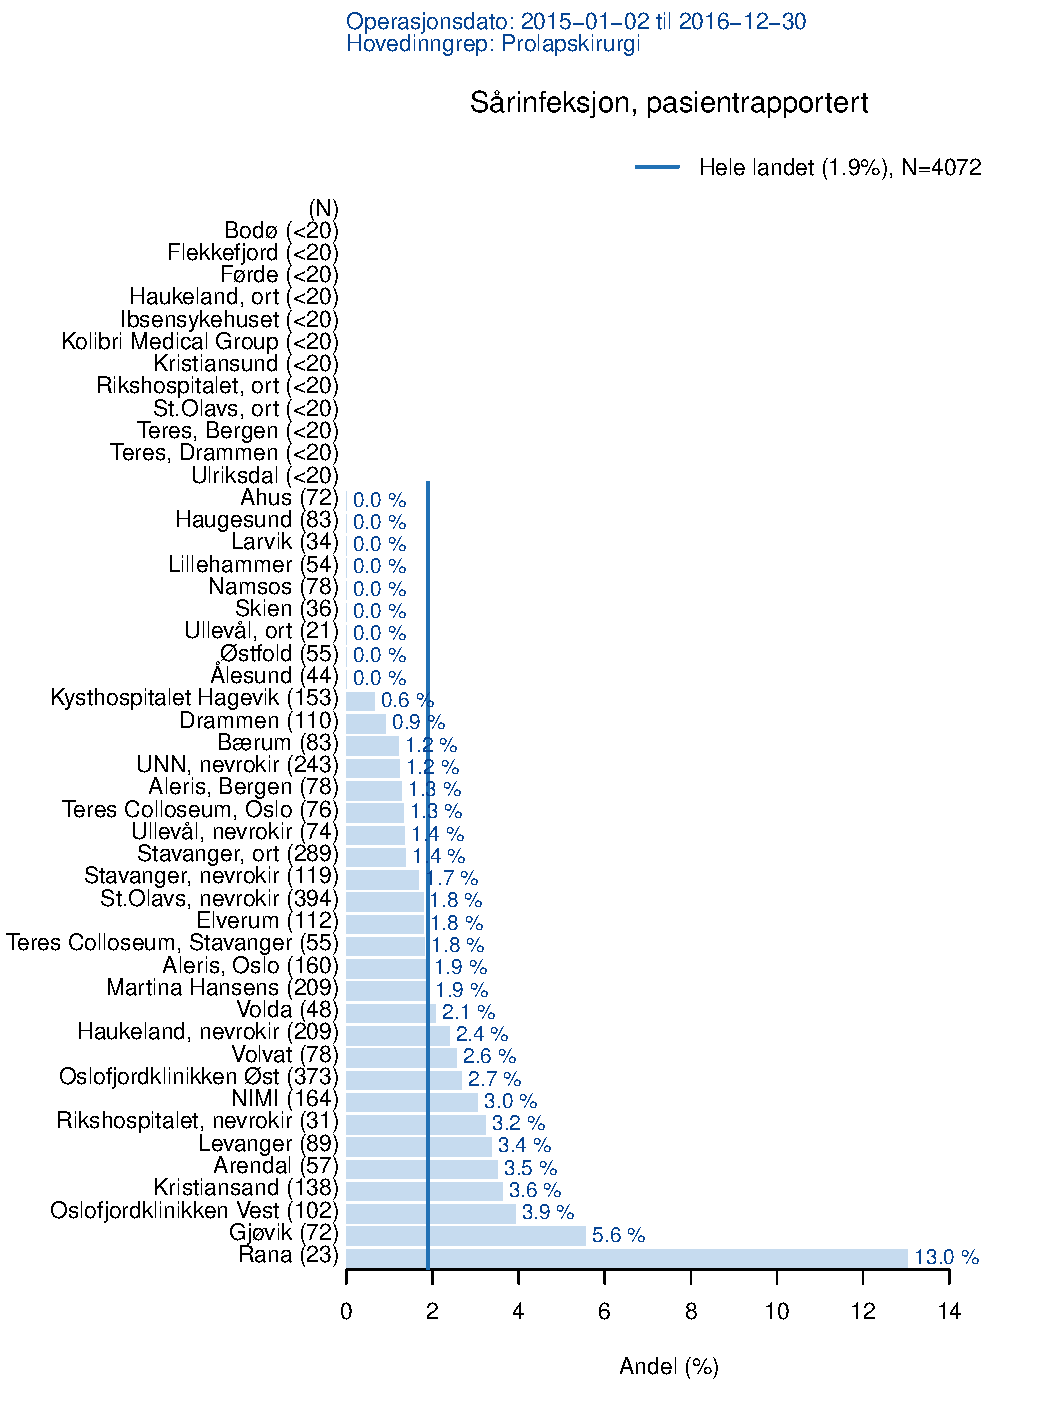
\includegraphics{Figurer/FigKpInf3MndPro.pdf}}
\caption{\label{fig:KpInfAvdPro} Andel pasienter som rapporterer om sårinfeksjon 3 måneder etter
prolapskirurgi.}
\end{figure}

\begin{figure}[ht]
\scalebox{0.7}{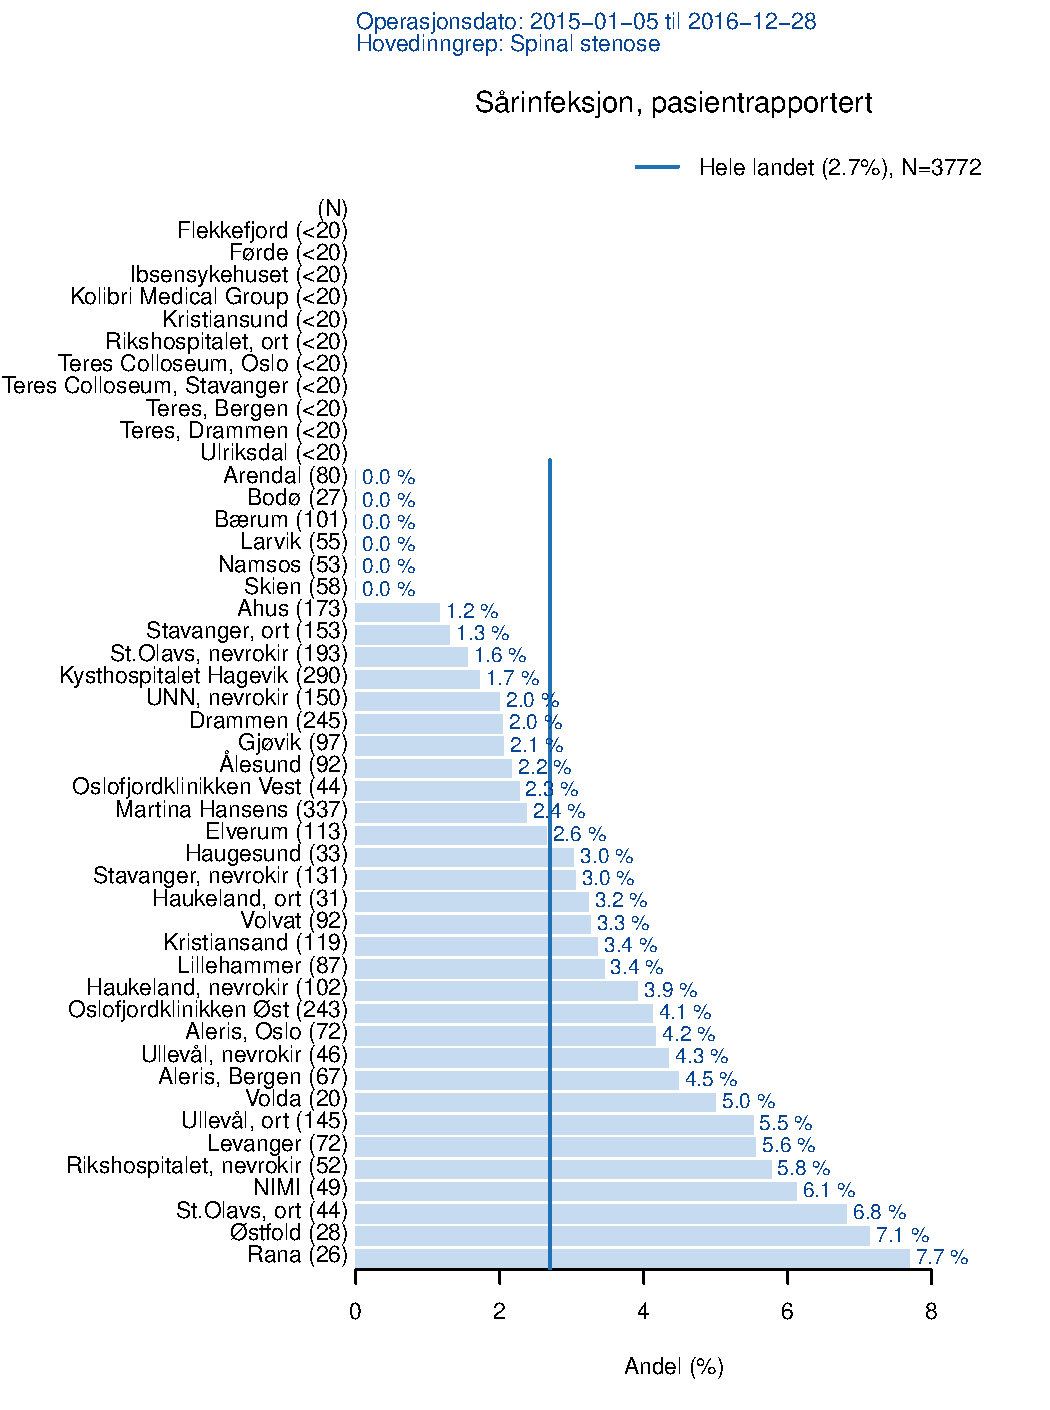
\includegraphics{Figurer/FigKpInf3MndSS.pdf}}
\caption{\label{fig:KpInfAvdSS} Andel pasienter som rapporterer om sårinfeksjon 3 måneder etter
spinal stenose.}
\end{figure}

%\clearpage



Durarift er oftest en ufarlig komplikasjon, men kan medføre væskelekkasje og
ubehag for pasienten, lengre liggetid og i noen tilfeller behov for reoperasjon.
Unntaksvis kan også konsekvensen være nerveskade og alvorlig infeksjon. Figur \ref{fig:Dura} viser andelen som får durarift for prolaps og spinal stenose pasienter.

\begin{figure}[ht]
\centering 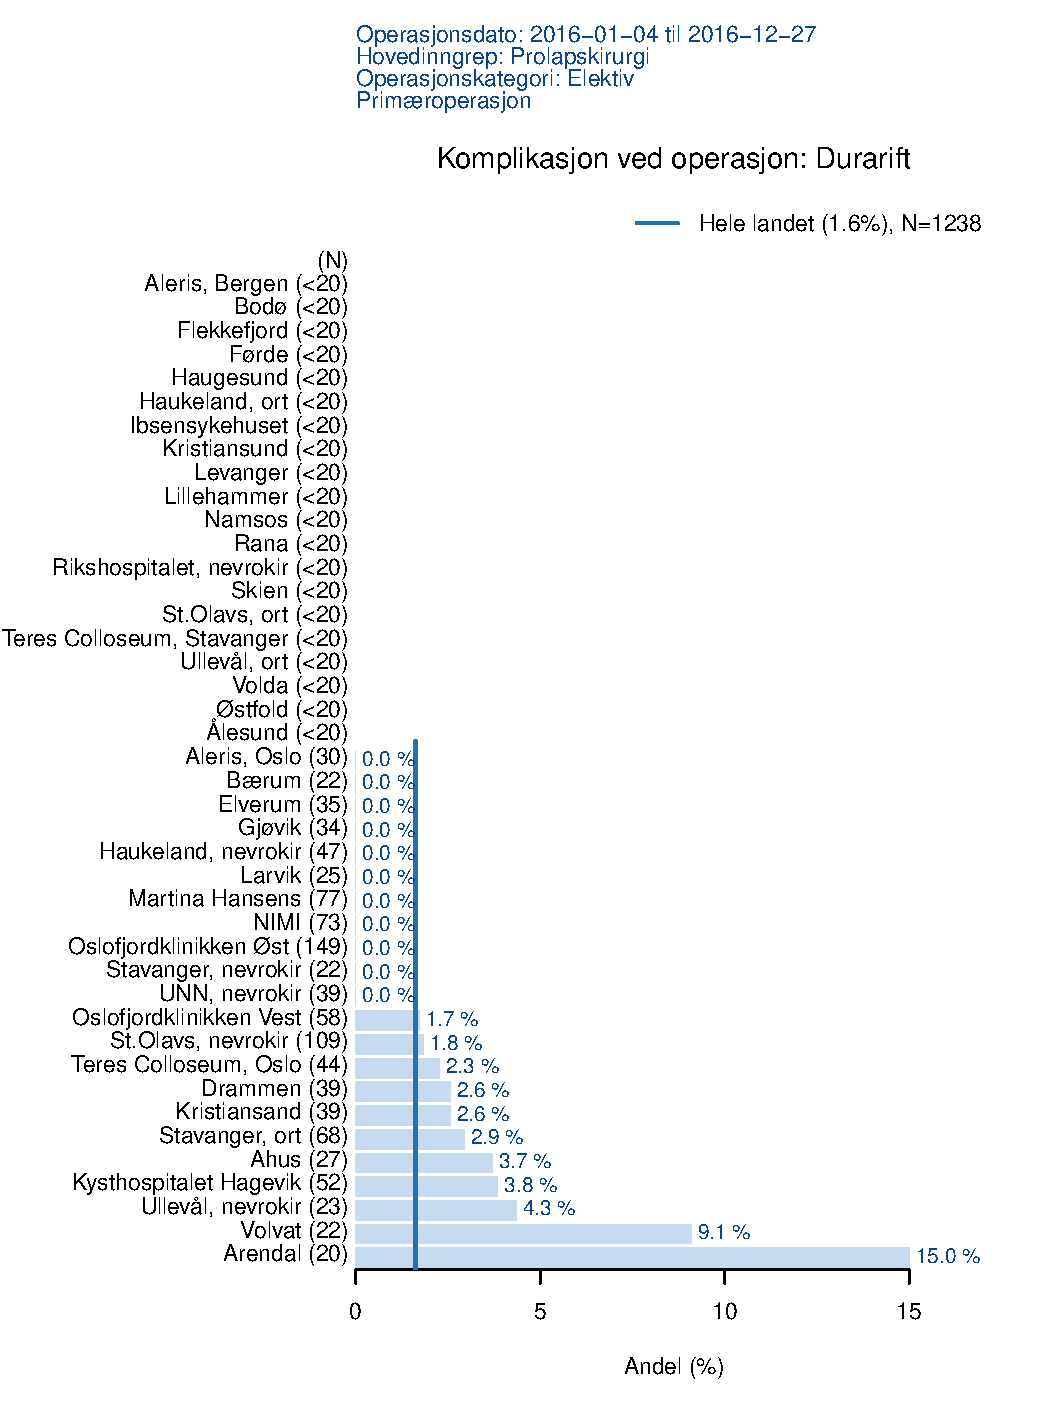
\includegraphics[width= 0.55\textwidth]{Figurer/FigDuraPro.pdf}
\centering 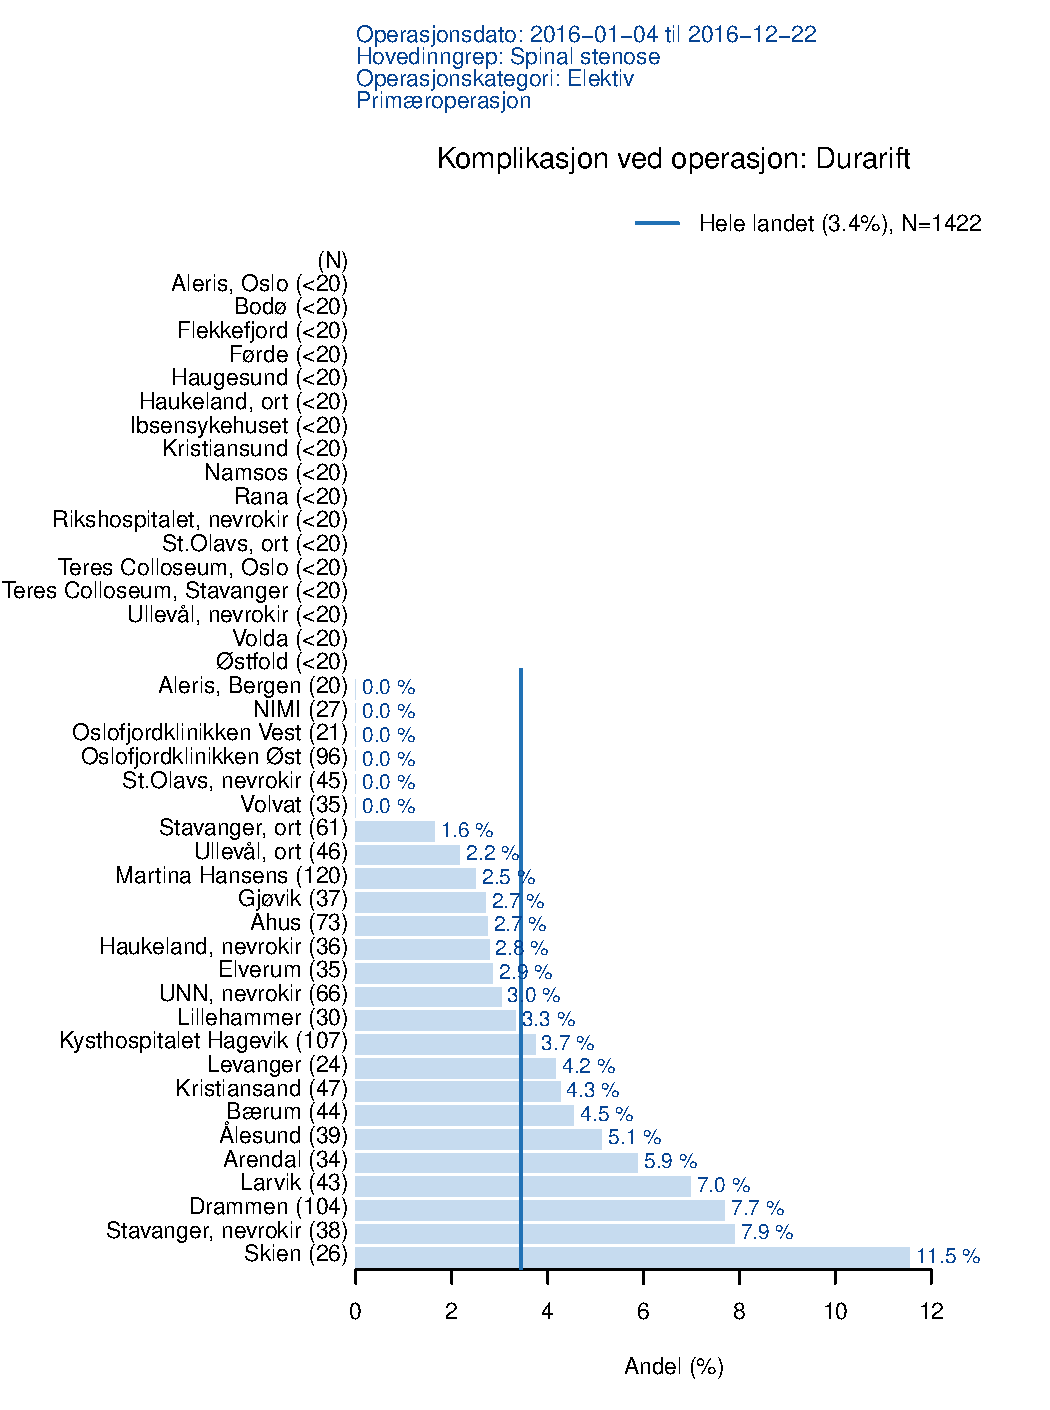
\includegraphics[width= 0.55\textwidth]{Figurer/FigDuraSS.pdf}
\caption{\label{fig:Dura} Andel pasienter som får durarift etter kirurgi for hhv. prolaps og spinal stenose, begge elektiv primæroperasjon.}
\end{figure}

























\clearpage

\section{Resultater degenerativ nakke}

I Norge drives nakkekirurgi kun ved nevrokirurgiske avdelinger knyttet til de fem
universitetssykehusene i Oslo, Bergen, Trondheim, Stavanger og Tromsø, samt ved
hovedsakelig ett privat sykehus (Oslofjordklinikken).
Da der ikke finnes etablerte kvalitetsindikatorer for nakkekirurgi vil dette bli en
viktig oppgave for NKR. Da en ny validering av datakvaliteten ikke er fullført grunnet
uventede databaseproblemer, vises kun et generelt mål på pasient rapporterte
tilfredshet (PREM) i årets rapport. I neste årsrapport vil NKR presentere sykehusvise
kvalitetsdata splittet på diagnose, behandling.
Pasienttilfredshet (PREM)



Figurer:
\begin{itemize}
\item Andel over 70 år per sykehus
\item Klart bedre
\item Stemmevansker, 3mnd
\item Svelgvansker, 3 mnd
\item Bruk alle år
\item Splitt på Myelopati/ikke
\item Splitte på fremre og bakre tilgang
\end{itemize}



Pasienter som opereres i nakken for degenerative tilstander har armsmerte med
eller uten funksjonssvikt (radikulopati), varierende grad av nakkesmerter og noen
har ryggmargspåvirkning (myelopati). Som hovedregel kan ikke pasienter som
opereres på grunn av ryggmargspåvirkning påregne bedring i samme grad som de
som behandles for armsmerte. Figur 3.21 viser at også andelen som opereres for
myelopati varierer mellom sykehusene.



\section{Oppsummering av de viktigste resultatene}







\end{document}
